

\section{Introduction}

Pour comprendre un système biologique, il est nécessaire d'étudier les interactions chimiques qui s'y déroulent.
Au delà du simple catalogage qui peut en être fait, comprendre les actions moléculaires permet d'utiliser ou même d'inventer de nouvelles substances pour l'industrie.
Afin d'explorer ces activités, un postulat simple a été posé : deux molécules proches ont deux activités proches.
Ce postulat simple parait raisonnable puisqu'il s'appuie sur le fait que l'activité d'une molécule est portée par la configuration spatiale des différents éléments qui la composent.
On sait aujourd'hui que ce postulat est en partie faux car on connaît quelques contre-exemples~\cite{patani_bioisosterism:_1996}.
Cependant, dans la majorité des cas, cette approximation fonctionne bien et tout un domaine de chemoinformatique s'est développé dans ce sens.
Toutes les techniques cherchant à rapprocher les structures des activités moléculaires sont regroupées derrière l'acronyme QSAR (Quantitative structure-activity relationship).
Les techniques QSAR sont nombreuses et de types variées~\cite{patani_bioisosterism:_1996,leach_molecular_2001,helma_predictive_2005}.
Certaines s'attardent sur les ressemblances de structures atomiques 2D ou 3D, certaines sur les propriétés magnétiques, d'autres sur les contraintes de repliement etc.
Beaucoup ne se cantonnent pas à une seule des ressemblances citées ci-dessus mais essaient de les combiner pour prédire au mieux l'activité.
Cependant, ces techniques ont deux limites.
Premièrement, pour déterminer l'activité d'une molécule, il est nécessaire de connaître les activités de molécules ``proches'', qu'il faut donc avoir annoté auparavant.
Deuxièmement, les temps de calcul nécessaires augmentent rapidement avec le nombre de critères à comparer et la complexité d'analyse de ceux-ci.
Le but de ces méthodes est donc d'inclure d'abord les critères les plus sélectifs afin de déterminer des activités connues en un temps raisonnable.

Beaucoup de NRP possèdent des activités très intéressantes (antibiotiques, anti-tumeurs, antidouleurs, ...).
À ce titre, nous cherchons en permanence à caractériser les activités de chaque nouvelle molécule découverte.
Lorsque ces activités ne sont pas déterminées expérimentalement, les logiciels exploitant des techniques de type QSAR permettent d'effectuer une prédiction.
En 2012 puis 2014, Abdo et al. publient de nouvelles méthodes de prédiction d'activité NRP, se basant sur les spécificités des NRP~\cite{abdo_new_2012, abdo_prediction_2014}.
Dans les deux cas, les prédictions sont effectuées à partir des compositions monomériques et non pas atomiques.
Dans le premier article~\cite{abdo_new_2012}, la prédiction est effectuée en créant pour chaque activité connue un \textit{fingerprint}.
Ces fingerprints sont les barycentres des peptides présentant l'activité.
Prédire l'activité d'un nouveau NRP revient alors à déterminer le barycentre d'activité le plus proche.
Dans le second article~\cite{abdo_prediction_2014}, c'est un classifieur par réseau Bayésien qui est entraîné sur les compositions en monomères.
Une fois les réseaux entraînés, il suffit de fournir une composition en entrée pour avoir les probabilités de chaque activité en sortie.
Dans les deux cas, il est important de constater que l'abstraction monomérique est suffisante pour une prédiction de qualité.
De plus, les structures des molécules ne sont pas utilisées, ce qui laisse encore beaucoup de possibilités d'améliorations.

Ce que nous venons de montrer par cet exemple de prédiction d'activité, c'est l'importance de la détermination des structures plus proches de la réalité biologique comme les structures monomériques.
Connaître ce type de structure est un enjeu fort pour la détermination de caractéristiques moléculaires haut niveau (activité ou conformation 3D par exemple).
Comme nous l'avons fait remarqué précédemment, il n'existe que peu d'outils permettant des annotations fiables de NRP.
Les caractérisations fiables de NRP sont en très grande majorité effectuées manuellement par des biologistes et chimistes.
Beaucoup de structures atomiques sont également connues sans annotations monomériques malgré leur présence dans de grandes bases de données.
Il nous a donc paru nécessaire de créer un outil qui infère la structure monomérique à partir d'une structure atomique et c'est cet outil d'annotation que nous allons décrire durant ce chapitre.




\section{Formalisation du problème d'annotation}

\label{problems}

\subsection{Définition du problème}

Nous cherchons à créer un outil bioinformatique permettant l'obtention de nouvelles annotations monomériques NRP fiables.
La génération d'annotations peut se baser sur la recherche d'informations à partir des gènes ou à partir des molécules dont pour lesquelles on connaît déjà la structure.
Dans notre cas, nous n'avons pas choisi de démarrer des clusters de gènes NRPS puisque des modèles déjà bien éprouvés existent (NRPSpredictor, NaPDoS, ...).
Les avancées dans ce domaines viendront avec le nombre d'annotations fiables de binômes clusters/NRP qui permettrons l'amélioration des modèles d'apprentissage actuels.

\begin{figure}[!ht]
  \begin{center}
    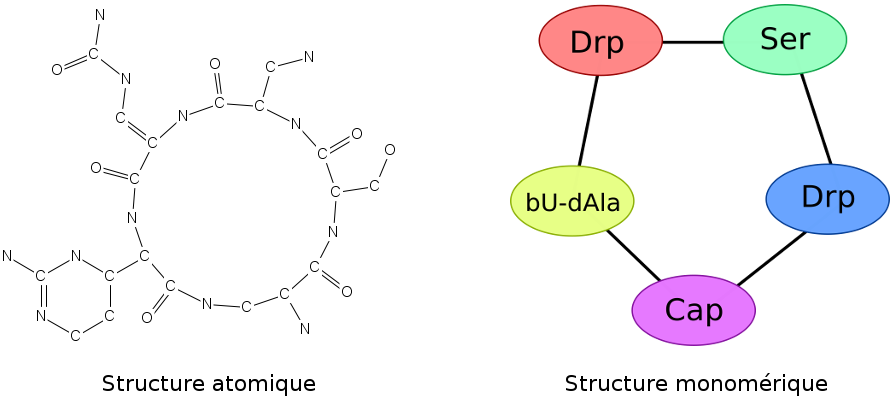
\includegraphics[width=400px]{Figures/s2m/Intro/structures.png}
    \caption{\label{structures}Structures atomique et monomérique de la Caprieomycin IIA.}
  \end{center}
\end{figure}

Dans notre cas, nous allons partir des structures atomiques pour déduire les composants monomériques (voir figure \ref{structures}).
De telles structures sont présentes dans de nombreuses bases de données publiques, telles que PDB ou PubChem.
Ces bases contiennent de nombreuses descriptions de molécules NRP sans annotations monomériques directement accessibles.
Notre objectif sera d'être capable, pour toute structure moléculaire NRP, de déduire sa composition en monomères.
Ainsi, toutes les structures atomiques présentes dans les bases généralistes pourront être annotées et ajoutées à des bases spécialisées telles que Norine.
Ce type d'annotation pourra également être effectué pour mettre en relation les structures atomiques non annotées des bases généralistes avec les annotations non liés des bases spécialisées.



\subsection{L'existant}

Parmi l'existant, la méthode CHUCKLES~\cite{siani_chuckles:_1994} et le logiciel molBLOCKS~\cite{ghersi_molblocks:_2014} se démarquent des autres.
Dans les deux cas, les logiciels permettent, à partir d'une structure atomique d'un polymère, de trouver la structure monomérique.
Les deux logiciels sont opposés dans leur façon de traiter le problème.
CHUCKLES est constructif car il part des monomères pour reconstituer le polymère alors que molBLOCKS est destructif car il part du polymère pour retrouver les monomères par découpes successives de liens.
Nous allons ici présenter ces deux approches.


\subsubsection{CHUCKLES, une méthode constructive}

CHUCKLES~\cite{siani_chuckles:_1994} est une méthode publiée en 1994 pour la recherche des peptides au sein d'une base de données.
Le but est de requêter une base de données de molécules en utilisant des expressions régulières entrées par l'utilisateur et représentant des sous-molécules d'intérêt.
Les recherches peuvent être effectuées à la fois au niveau atomique et au niveau monomérique.
Le but de CHUCKLES est de convertir rapidement les données du format monomérique vers le format atomique et inversement.
Les auteurs pensent qu'il est plus utile de conserver les formats atomiques en base plutôt que les séquences protéiques.
Sachant que la plupart des peptides de l'époque étaient déjà représentés par leur séquence, les auteurs proposent une méthode de transformation vers la structure atomique.
Cette transformation est appelée ``Forward-Translation'' (FT).

\begin{figure}[!ht]
  \begin{center}
    \includegraphics[width=450px]{Figures/s2m/formalisation/CHUCK_FT.png}
    \caption{\label{chuck_ft}CHUCKLES Forward Translation.
    Transformation des annotations peptidiques en SMILES.
    Sous l'annotation peptidique est écrite la formule SMILES après concaténation de tous les SMILES des monomères trouvés.
    Schémas issus de la publication}
  \end{center}
\end{figure}

Pour mener à bien chaque FT, les auteurs utilisent une table de transformation qui recense les structures atomiques de chacun des monomères à transformer.
Chaque structure ne doit pas contenir les atomes qui vont être perdus lors des liaisons avec d'autres monomères.
Pour les structures linéaires, la méthode propose une simple concaténation des structures atomiques selon la chaîne peptidique.
Lorsque les structures sont branchées ou cycliques, il est nécessaire d'ajouter dans la structure initiale l'information de liaison annexe.

Cette méthode de reconstruction des structures atomiques est très intéressante mais souffre du manque d'information sur le sens des monomères inclus.
On peut remarquer que la reconstruction ne peut fonctionner à tous les coups sans cette d'information.
En effet, si les monomères ne possèdent pas un groupement carboxyl et un amine, le sens de naturel des liaisons peptidique ne peut être retrouvé.
La reconstruction se fait alors en utilisant un sens aléatoire pour le monomère.

\begin{figure}[!ht]
  \begin{center}
    \includegraphics[width=300px]{Figures/s2m/formalisation/CHUCK_BT.png}
    \caption{\label{chuck_bt}CHUCKLES Backward Translation.
    La première partie représente la phase de recherche des monomères au sein de la structure atomique.
    La seconde partie représente la structure monomérique post contraction.
    On peut voir à gauche la chaîne principale qui a été extraite à partir du N initial.
    A droite sont répertoriés les deux ponts disulfure extraits hors de la chaîne principale.
    Chaque monomère découvert comporte un identifiant différent de son nom pour éviter d'avoir deux fois le même nom comme cela pourrait être le cas ici.
    Schémas issus de la publication~\cite{siani_chuckles:_1994}}
  \end{center}
\end{figure}

La seconde partie de la méthode, précisément celle qui nous concerne, présente la transformation inverse (``Backward-Transformation'' (BT)).
C'est cette partie qui est très intéressante pour l'annotation car elle part des structures atomiques pour reconstruire les structures monomériques.
Les auteurs proposent une annotation en deux temps.
Une phase de recherche des monomères, puis une conversion des monomères trouvés en une annotation.
L'idée de la première phase est de rechercher chaque monomère connu en masquant les atomes déjà utilisés par des monomères précédemment trouvés.
En recherchant les monomères par taille (nombre d'atomes) décroissante, les auteurs s'assurent que de petits monomères ne viendront pas prendre la place de plus gros.
C'est un algorithme glouton sans aucun retour arrière.
Lors de la seconde phase, les atomes des molécules sont contractés pour ne plus former qu'un seul n\oe{}ud par monomère.
Le N terminal de la chaîne peptidique est ensuite recherché afin d'extraire l'annotation de cette chaîne en suivant les liaisons peptidiques.
Enfin, les liaisons n'ayant pas encore été explorées sont ajoutées à la représentation monomérique finale.

Comme pour le FT, le BT utilise des techniques intelligentes mais encore faillibles.
Dans le cas des NRP, certains monomères ne possèdent pas les deux domaines pour les liaisons peptidiques.
Il est donc potentiellement impossible de retrouver une chaîne principale.
De plus, lors de la recherche, si les monomères à rechercher sont structurellement proches, il est possible qu'un gros monomère vienne prendre la place d'un plus petit en débordant sur un ou plusieurs monomères voisins.
Dans ce cas, vu qu'aucun retour en arrière n'est effectué, l'annotation sera inexacte voir incomplète.


\subsubsection{molBLOCKS, une méthode destructive}

\begin{figure}[!ht]
  \begin{center}
    \includegraphics[width=400px]{Figures/s2m/Intro/molBlocks.png}
    \caption{\label{molBlocks}Application de la méthode molBlocks sur le polymère ACV.
    Le polymère est séparé en morceau par une règle de liaison peptidique.
    Les trois morceaux correspondent aux trois monomères réellement inclus, la découpe fonctionne.}
  \end{center}
\end{figure}

Le logiciel molBLOCKS~\cite{ghersi_molblocks:_2014} n'est, à la base, pas conçu pour le travail que nous cherchons à effectuer.
C'est un logiciel qui permet de découvrir des monomères en repérant les fragments fréquents au sein d'une population de polymères.
Pour cela le logiciel découpe les polymères en petits fragments et effectue des comptages de ceux-ci.
Ces découpes suivent des règles entrées par l'utilisateur.
Par exemple en donnant comme règle
\begin{equation}
  O=CNH \longrightarrow C=O + NH
\end{equation}
toutes les liaisons peptidiques seront ciblées et déconnectées (voir figure \ref{molBlocks}).
Pour des protéines ribosomiques, la découpe sera donc parfaite avec cette seule règle et les monomères seront découverts.

\begin{figure}[!ht]
  \begin{center}
    \includegraphics[width=300px]{Figures/s2m/Intro/molBlocks_problem.png}
    \caption{\label{molBlocks_problem}Dans le cas de ce di-peptide, un sucre est lié à une Hydroxy-Phenil-Glycine (Hpg).
    En utilisant la règle de découpe à appliquer pour les hydroxyl, une ambiguïté et une erreur apparaissent.
    Nous ne pouvons savoir de quel côté les découpes vont être les plus pertinentes avant d'essayer de reconnaître les monomères.
    De ce fait, 4 découpes différentes sont possibles.
    De plus, le cycle du sucre se voit ouvert alors que la découpe est inutile.}
  \end{center}
\end{figure}

Dans notre cas, nous pourrions utiliser un tel logiciel pour découper les NRP en monomères.
En effectuant par la suite une étape de reconnaissance de ces monomères, il serait alors possible de reconstruire le peptide.
Cependant, certaines réactions effectuées au sein des NRP ne permettent pas de découper entièrement le peptide avec la seule règle énoncée précédemment.
Toutes les liaisons non peptidiques énoncées au chapitre précédent ne seront pas découpées.
Il est donc nécessaire de rajouter de nouvelles règles.
Cependant, la liaison hydroxyl à elle seule ne permet déjà plus d'effectuer une découpe correcte.
Pour pouvoir la délier, il faudrait une règle du type
\begin{equation}
  COC \longrightarrow CO + C
\end{equation}
Mais ce genre de règle est ambiguë.
Il est impossible de connaître de quel côté du O la liaison doit être rompue.
De plus, certains monomères comme le glucose sont initialement composés de $COC$.
Ces monomères seront donc découpés alors qu'ils ne devraient pas l'être.
Pour ces deux raisons, nous ne pourrons pas directement utiliser ce logiciel afin de convertir nos structures atomiques en structures monomériques.
% 
% 
% \subsubsection{Vue générale}
% 
% En dehors des deux logiciels que nous venons de présenter, rien n'est dédié spécifiquement à la tâche que nous cherchons à accomplir.
% Un grand nombre de techniques que j'ai étudiées ne permettent que la résolution de sous problèmes.
% Par exemple, lors de la présentation de CHUCKLES, nous citons une implémentation des SMARTS appelée AMBIT-SMARTS.
% Les SMARTS sont des expressions régulières moléculaires qui permettent de définir des motifs à rechercher.
% En appliquant un SMARTS sur une molécule (comme le permet AMBIT-SMARTS), nous pouvons savoir si cette molécule contient ce motif.
% Ce type de technique permet de savoir si une molécule est contenue dans une autre, ce qui dans notre cas reviendrait à savoir si un monomère est contenu dans un polymère.
% Cette tâche très importante n'est pas suffisante pour répondre à nos attentes, mais peut éventuellement faire partie des sous techniques à utiliser.




\subsection{Vers des problèmes informatiques}

Pour concevoir notre logiciel d'annotation, nous allons nous inspirer des techniques existantes en essayant de dépasser leurs difficultés.
Nous possédons, au sein de Norine, une grande base de connaissances de monomères existants (plus de 500) et nous pouvons nous appuyer sur cette base bien établie pour assurer l'existence des monomères lors des annotations.
A partir de ces données, essayons de concevoir un algorithme constructif.


\subsubsection{Une histoire de sous problèmes}
\label{subproblems}

La méthode CHUCKLES tire partie de la différence entre les 20 acides aminés principaux pour se permettre de rechercher les plus gros en premier et de ne jamais revenir sur les choix faits.
Rechercher les monomères par taille (en nombre d'atomes) décroissante et en masquant les atomes déjà utilisés est un choix pertinent car il permet d'éviter de détecter partout les petits acides aminés comme la glycine.
Dans notre cas, la proximité entre certains monomères ne nous permettra pas de les départager grâce à un tri par taille.
Nous risquons d'introduire de trops gros monomères prenant la place d'autres et créant artificiellement des ``trous'' dans l'annotation.
Il sera nécessaire de modifier les solutions incomplètes pour essayer de les améliorer.
Contrairement à CHUCKLES, nous aurons donc besoin de connaître les différents monomères candidats à la composition du polymère même lorsqu'ils sont chevauchants à des monomères déjà placés.
Si d'un côté nous recherchons les monomères au sein du NRP, puis de l'autre nous assemblons ceux trouvés, alors nous pouvons séparer notre programme en deux sous-problèmes complètement distincts.

\begin{figure}[!ht]
  \begin{center}
    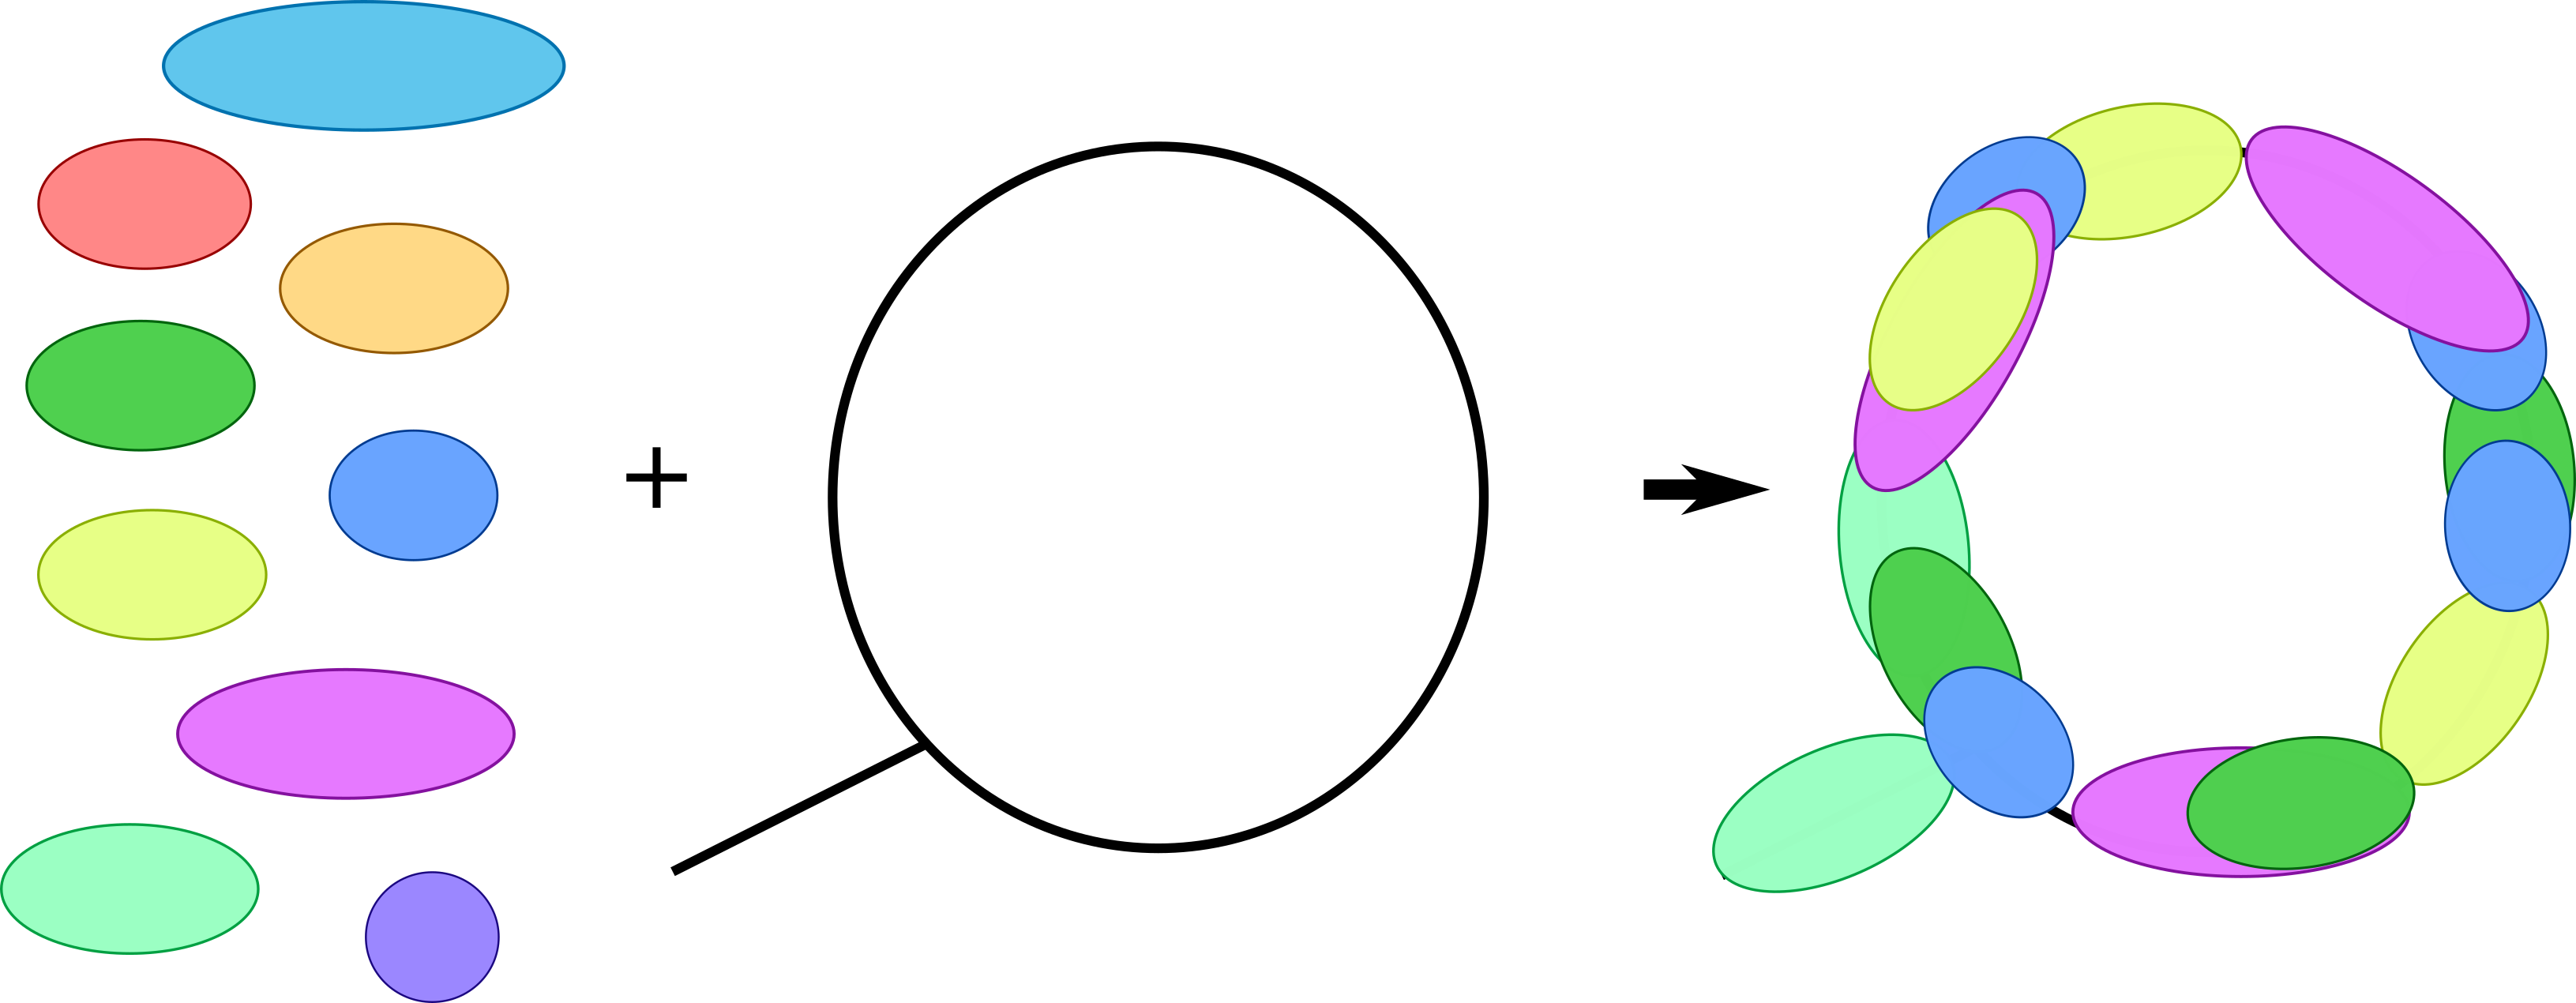
\includegraphics[width=400px]{Figures/s2m/Intro/searching.png}
    \caption{\label{search_fig}Première étape : Recherche des monomères (ellipses colorées) sur le peptide à annoter (cycle noir branché).}
  \end{center}
\end{figure}

Dans un premier temps, nous allons chercher à déterminer les monomères qui pourraient être les candidats pour composer le peptide étudié.
En utilisant la base Norine, nous pouvons indépendamment rechercher chacun des monomères connus au sein de la molécule à annoter.
La recherche exacte d'un monomère au sein d'un peptide est donc notre premier sous problème à résoudre.
Ce sous problème sera appelé la ``recherche'' (voir figure \ref{search_fig}).

\begin{figure}[!ht]
  \begin{center}
    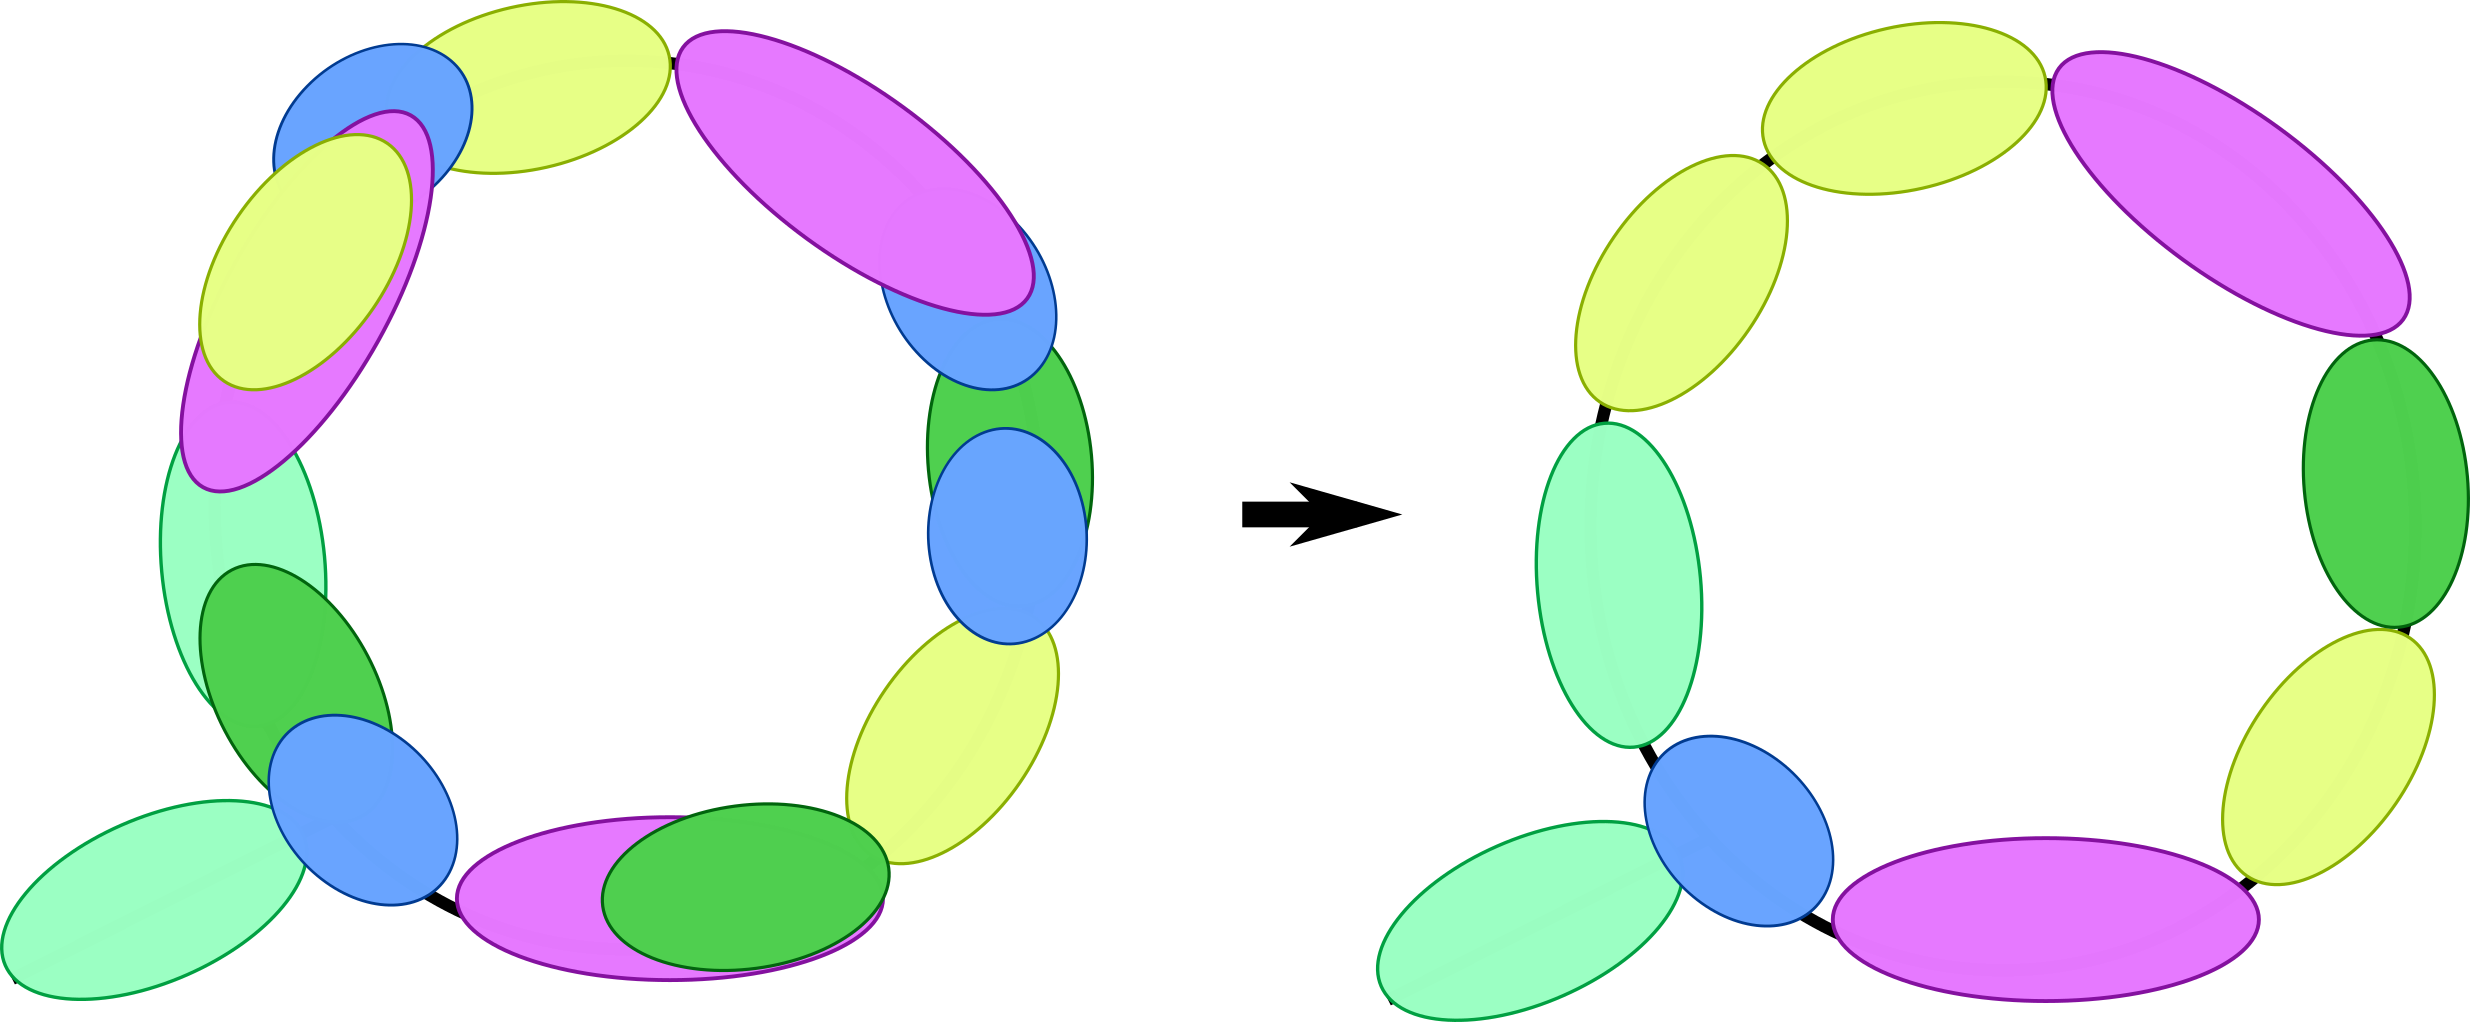
\includegraphics[width=400px]{Figures/s2m/Intro/tiling.png}
    \caption{\label{tiling_fig}Seconde étape : Sélection des monomères parmi ceux trouvés à l'étape 1.
    Le but est d'obtenir une structure monomérique non chevauchante de couverture maximale.}
  \end{center}
\end{figure}

Dans un second temps, nous devrons choisir parmi tous les monomères candidats issus de la recherche, lesquels composent réellement le polymère.
Nous aurons plusieurs contraintes associées à ce problème.
Aucun des monomères choisis dans la solution ne peut être chevauchant avec un autre.
En effet, aucun atome ne peut provenir de deux molécules différentes et donc aucune sous partie de monomères ne peut être chevauchante avec un autre monomère.
De plus nous allons chercher à obtenir une annotation complète des peptides, ce qui correspond à maximiser les atomes du polymère couverts par des monomères.
On appellera cette étape l'étape de ``pavage'' (voir figure \ref{tiling_fig}).

\subsubsection{Des molécules aux graphes}

Pour comprendre la suite du propos, il est nécessaire de comprendre ce qu'est un graphe au sens informatique du terme.
Pour plus de détails référez-vous au prérequis \ref{graphes}.


\subsubsection{Formalisation en problèmes de graphes}

Comme expliqué plus haut, le problème de recherche de sous composants d'un polymère peut être divisé en deux
plus petit problèmes : un problème de recherche de monomères et un problème de pavage des monomères trouvés. Traitons
donc séparément ces deux problèmes.

\textbf{Recherche de monomères}~~~
Rechercher un monomère dans un polymère revient à rechercher un petit graphe atomique
$S$ dans un plus gros graphe $G$. Deux cas sont alors possibles : soit nous cherchons à trouver exactement $S$ dans
$G$, soit nous cherchons une approximation de $S$ dans $G$. Dans le premier cas, nous allons nous intéresser à l'
``Isomorphisme de Sous-graphe'' (en anglais \textit{Subgraph Isomorphism} (SI)). Dans le second cas, nous nous intéresserons au
``Sous-graphe Maximum Commun'' (en anglais \textit{Maximum Common Subgraph} (MCS)). Les recherches de SI ou de MCS ont toutes
deux été prouvées NP-Complet mais, pour chacun des problème, il existe des algorithmes rapides en pratique pour des graphes
aux propriétés particulières.
Nous aborderons cela en section \ref{SI_MCS}.

\textbf{Pavage des monomères}~~~
Une fois les monomères détectés, il est nécessaire de choisir un monomère au sein des parties du polymère pour lequelles un conflit existe (plusieurs monomères possibles pour les mêmes atomes).
L'objectif est donc de faire un choix entre les différents morceaux possibles afin de chercher à ne garder que les pièces non chevauchantes qui permettent de couvrir au mieux le polymère, si possible dans sa totalité.
Ce genre de méthode est appelée ``pavage sans recouvrement''.
Cette étape donnant accès à un lien direct entre atomes et monomères, une étape de contraction de graphe permettra, au final, d'obtenir le graphe monomérique.




\section{Sous-graphe Maximum Commun vs Isomorphisme de Sous-graphe}
\label{SI_MCS}

Nous venons de voir que la recherche de monomères pouvait correspondre à deux problèmes différents en recherche de graphe.
Formalisons et étudions ici ces deux problèmes afin de choisir celui qui nous utiliserons au sein de notre logiciel d'annotations.
Voyons les différentes façons de les résoudre ainsi que les forces et faiblesses de ces approches.


\subsection{Sous-graphe Maximum Commun}

\subsubsection{Définition}

\begin{figure}[!ht]
  \begin{center}
    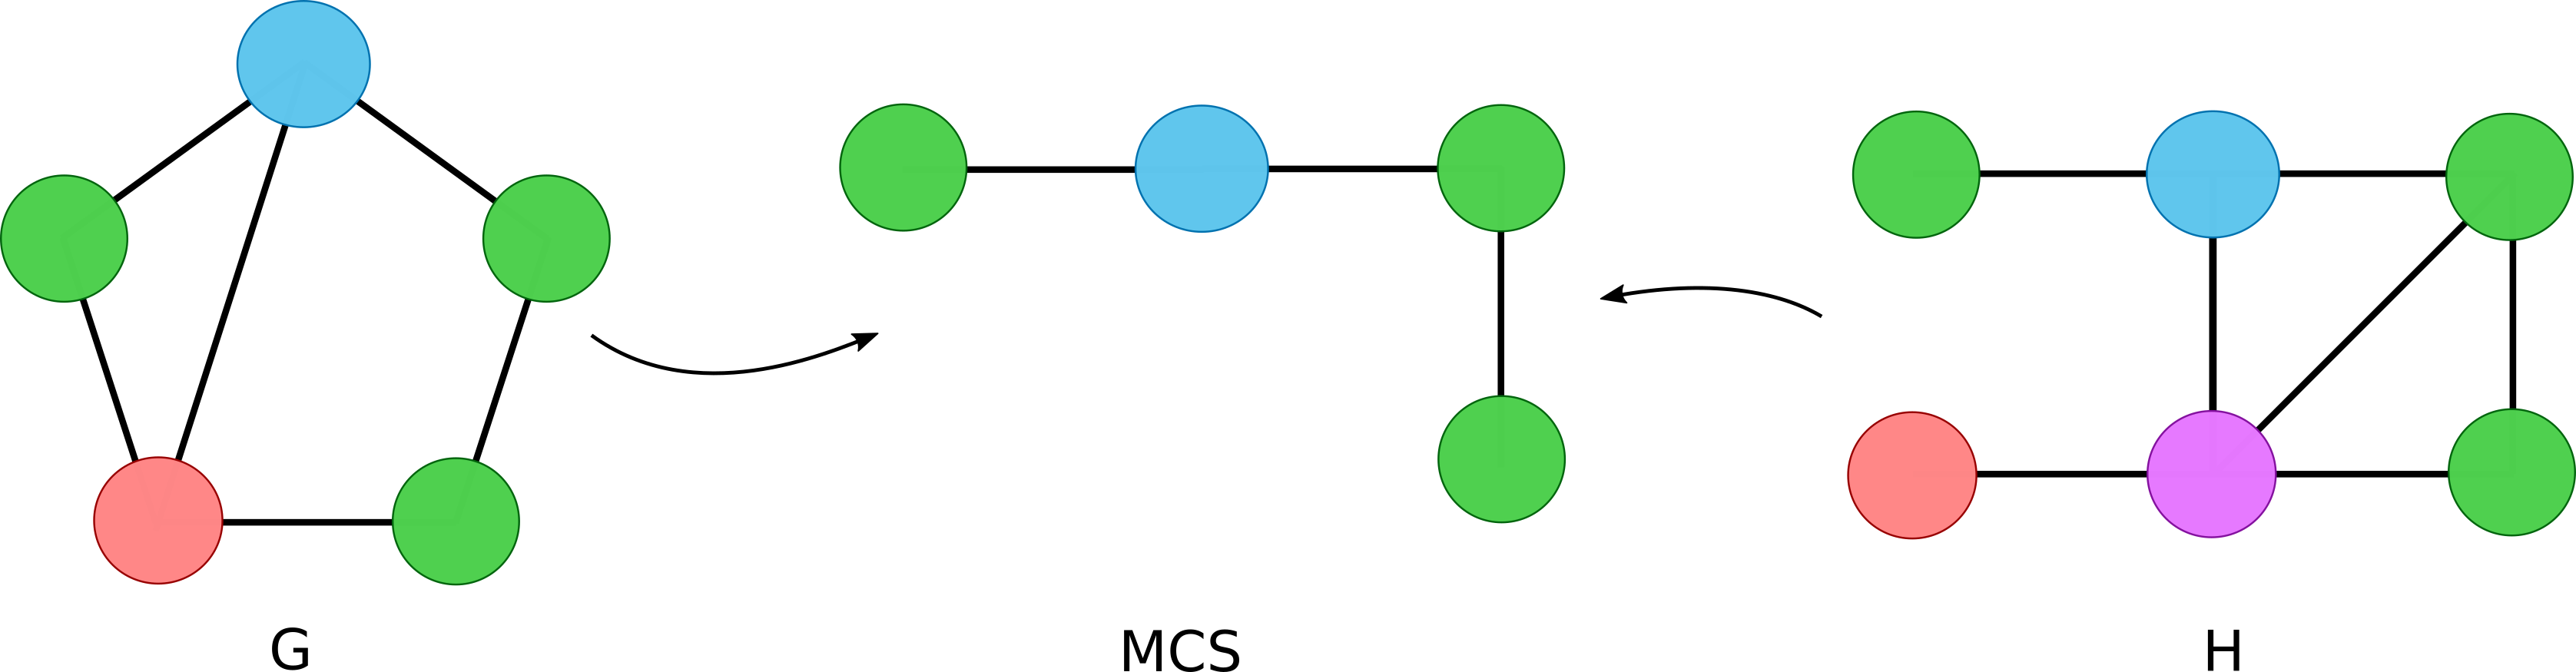
\includegraphics[width=450px]{Figures/s2m/MCS-SI/mcs.png}
    \caption{\label{mcs_fig}MCS obtenu à partir des graphes G et H.
    Le MCS obtenu ne contient pas le n\oe{}ud étiqueté ``rouge'' du fait des liens vers ce n\oe{}ud qui ne sont pas les mêmes dans G et H.}
  \end{center}
\end{figure}

Commençons par définir précisément le problème du MCS.
Comme le nom l'indique, le problème du MCS est un problème de recherche de la sous partie commune maximale entre deux graphes (Voir figure \ref{mcs_fig}).
C'est à dire trouver un ensemble de n\oe{}uds présents dans les deux graphes et dont les arêtes qui les inter-connectent sont présentes dans les deux graphes.
Il faut non seulement que les n\oe{}uds partagent les même étiquettes, mais également les mêmes voisins.
Si deux n\oe{}uds ont la même étiquette mais ne partagent pas les mêmes voisins dans les deux graphes, alors ils ne font pas partie du MCS.
C'est par exemple le cas du n\oe{}ud rouge au sein de la figure \ref{mcs_fig}.
Le problème de recherche de sous-graphe commun connexe maximal (MCCS) est un problème encore plus difficile, car il impose de fortes contraintes supplémentaires.
Le problème du MCS a été prouvé NP-Complet\cite{garey_computers_1979}, ce qui laisse peu de perspectives pour l'émergence d'algorithmes de résolution polynomiaux exacts.

Dans notre cas, nous pouvons effectuer une réduction vers ce problème pour la recherche des monomères.
Si l'on considère qu'un monomère et un polymère sont des graphes atomiques, alors trouver une sous partie commune à ces deux graphes revient à trouver un emplacement où une partie du monomère est retrouvée dans le peptide.
En imposant que le graphe commun soit d'une taille minimale fixée, nous pourrons éviter d'avoir des résultats ne contenant que quelques atomes par hasard.

Du fait de la NP-complétude du problème, trouver des solutions exactes est très compliqué.
Il existe tout de même quelques algorithmes de résolution exacts mais la majorité des articles à propos de MCS traitent d'heuristiques de résolution rapide.
Voyons ensemble ces deux catégories d'algorithmes en s'appuyant sur les reviews~\cite{raymond_maximum_2002, ehrlich_maximum_2011}.


\subsubsection{Les méthodes exactes de résolution}

Au sein des algorithmes de résolution exacte du MCS, il existe deux grandes écoles.
D'un côté, le problème du MCS est réduit en un problème de clique maximale, avant d'utiliser des solveurs dédiés à ce second problème.
D'un autre côté, les méthodes de résolution se basent sur des méthodes de backtracking.



\textbf{La réduction en clique maximale}~~~
Il est possible de réduire le problème MCS en un problème de résolution de clique maximale~\cite{pelillo_matching_1999,grosso_simple_2008,rahman_small_2009}.
Une clique est un ensemble de n\oe{}uds dans un graphe tel que tous les n\oe{}uds de cet ensemble sont reliés entre eux.
Rechercher la clique maximale revient à rechercher le sous ensemble maximal de n\oe{}uds d'un graphe pour lequel tous les n\oe{}uds sont liés les uns aux autres.
Il est possible d'obtenir plusieurs cliques maximales dans un même graphe.
Ce problème est également NP-Complet~\cite{akkoyunlu_enumeration_1973}.
Les résolutions de ce problème sont toutes des dérivées de la recherche exhaustive par backtracking.
Il est possible de ne pas passer par toutes les combinaisons possibles en réduisant l'espace de recherche en fonction de l'arité des n\oe{}uds ou de leur contexte local mais les algorithmes restent exponentiels~\cite{tomita_worst-case_2004}.

\begin{figure}[!ht]
  \begin{center}
    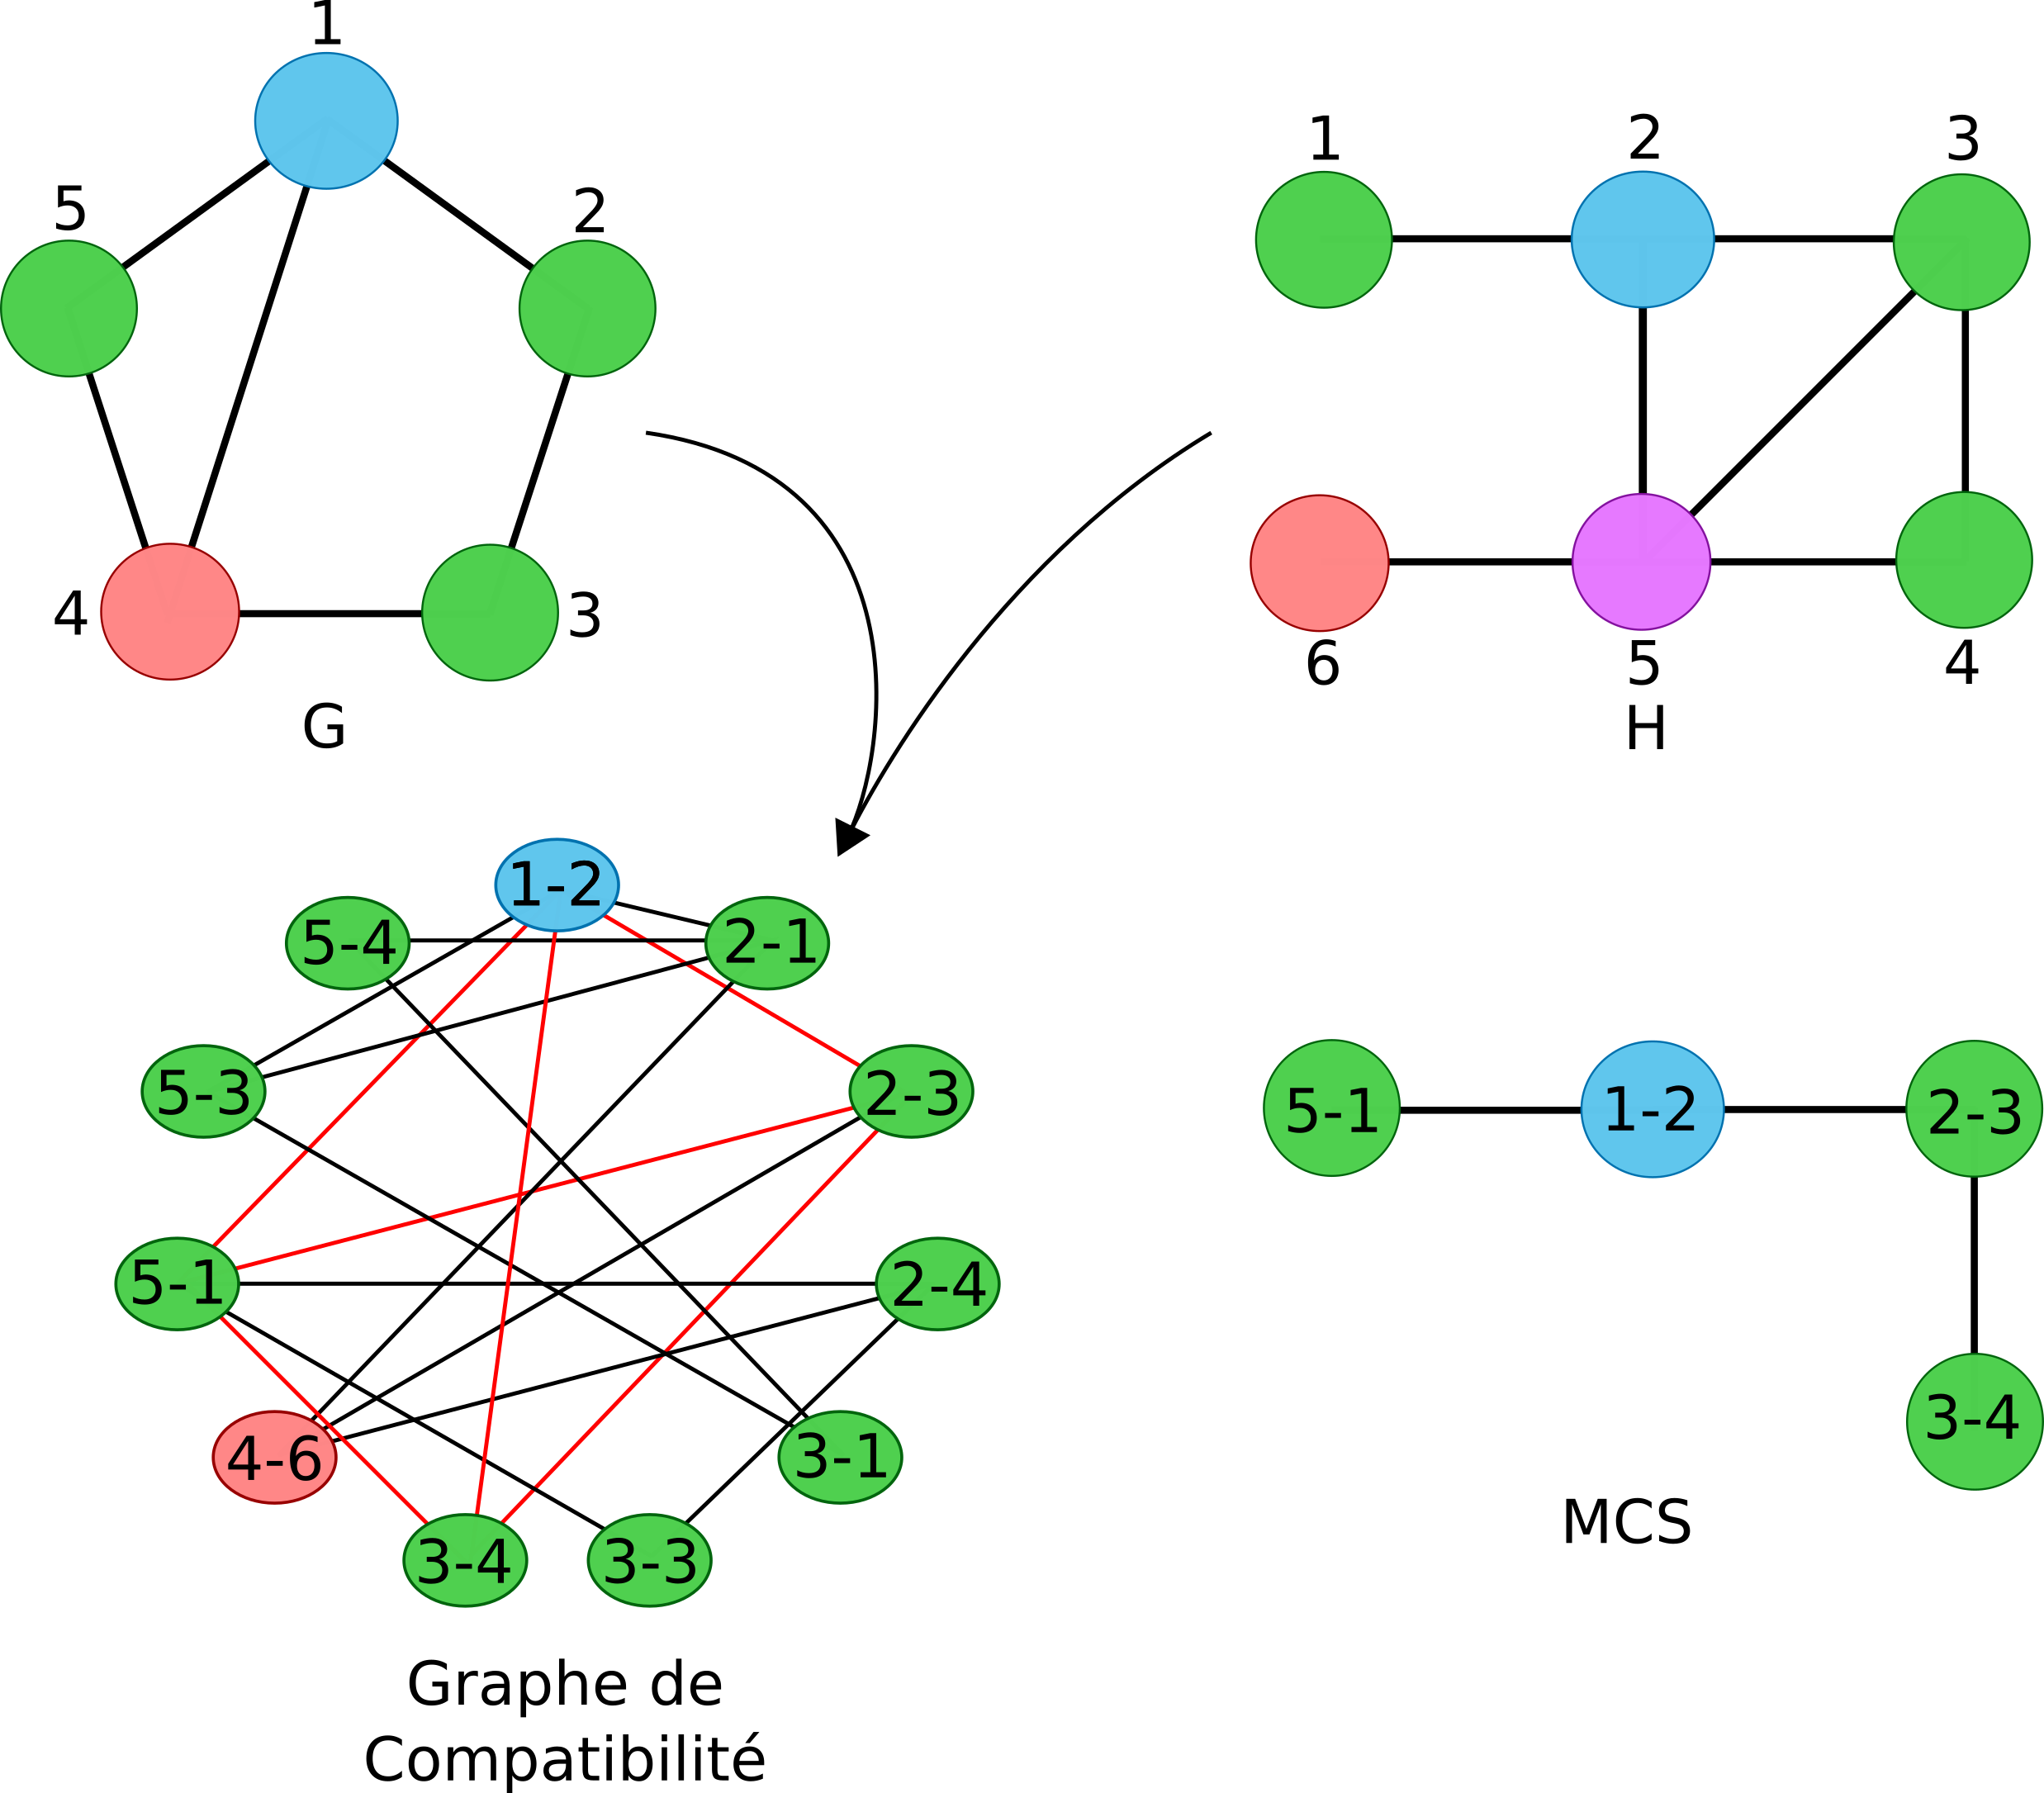
\includegraphics[width=400px]{Figures/s2m/MCS-SI/clique_solve.png}
    \caption{\label{clique_solve_fig}Résolution d'un MCS par réduction en clique maximale.
    Les couleurs représentent les étiquettes des noeuds.
    Dans le graphe de compatibilité les arêtes rouges identifient la clique maximale détectée.}
  \end{center}
\end{figure}

Pour obtenir un MCS à partir de solveur de clique maximale, il est nécessaire de construire un graphe de compatibilité (voir schéma \ref{clique_solve_fig}).
Un graphe de compatibilité (GC) est un graphe créé à partir du croisement des deux graphes (qu'on appellera G et H).
Pour les n\oe{}uds du GC, on génère tous les couples de noeuds $(x, y)$ possibles avec $x$ issu de G et $y$ de H et dont les étiquettes sont identiques.
Ensuite on ajoute une arête entre deux couples $(x_1 , y_1)$ et $(x_2 , y_2)$ de GC si $x_1$ est voisin de $x_2$ dans G et $y_1$ voisin de $y_2$ dans H.
On ajoute également une arête si les $x$ sont non voisins et les $y$ également.
En résolvant le problème de clique maximale sur le GC, on obtient le MCS.


\begin{figure}[!ht]
  \begin{center}
    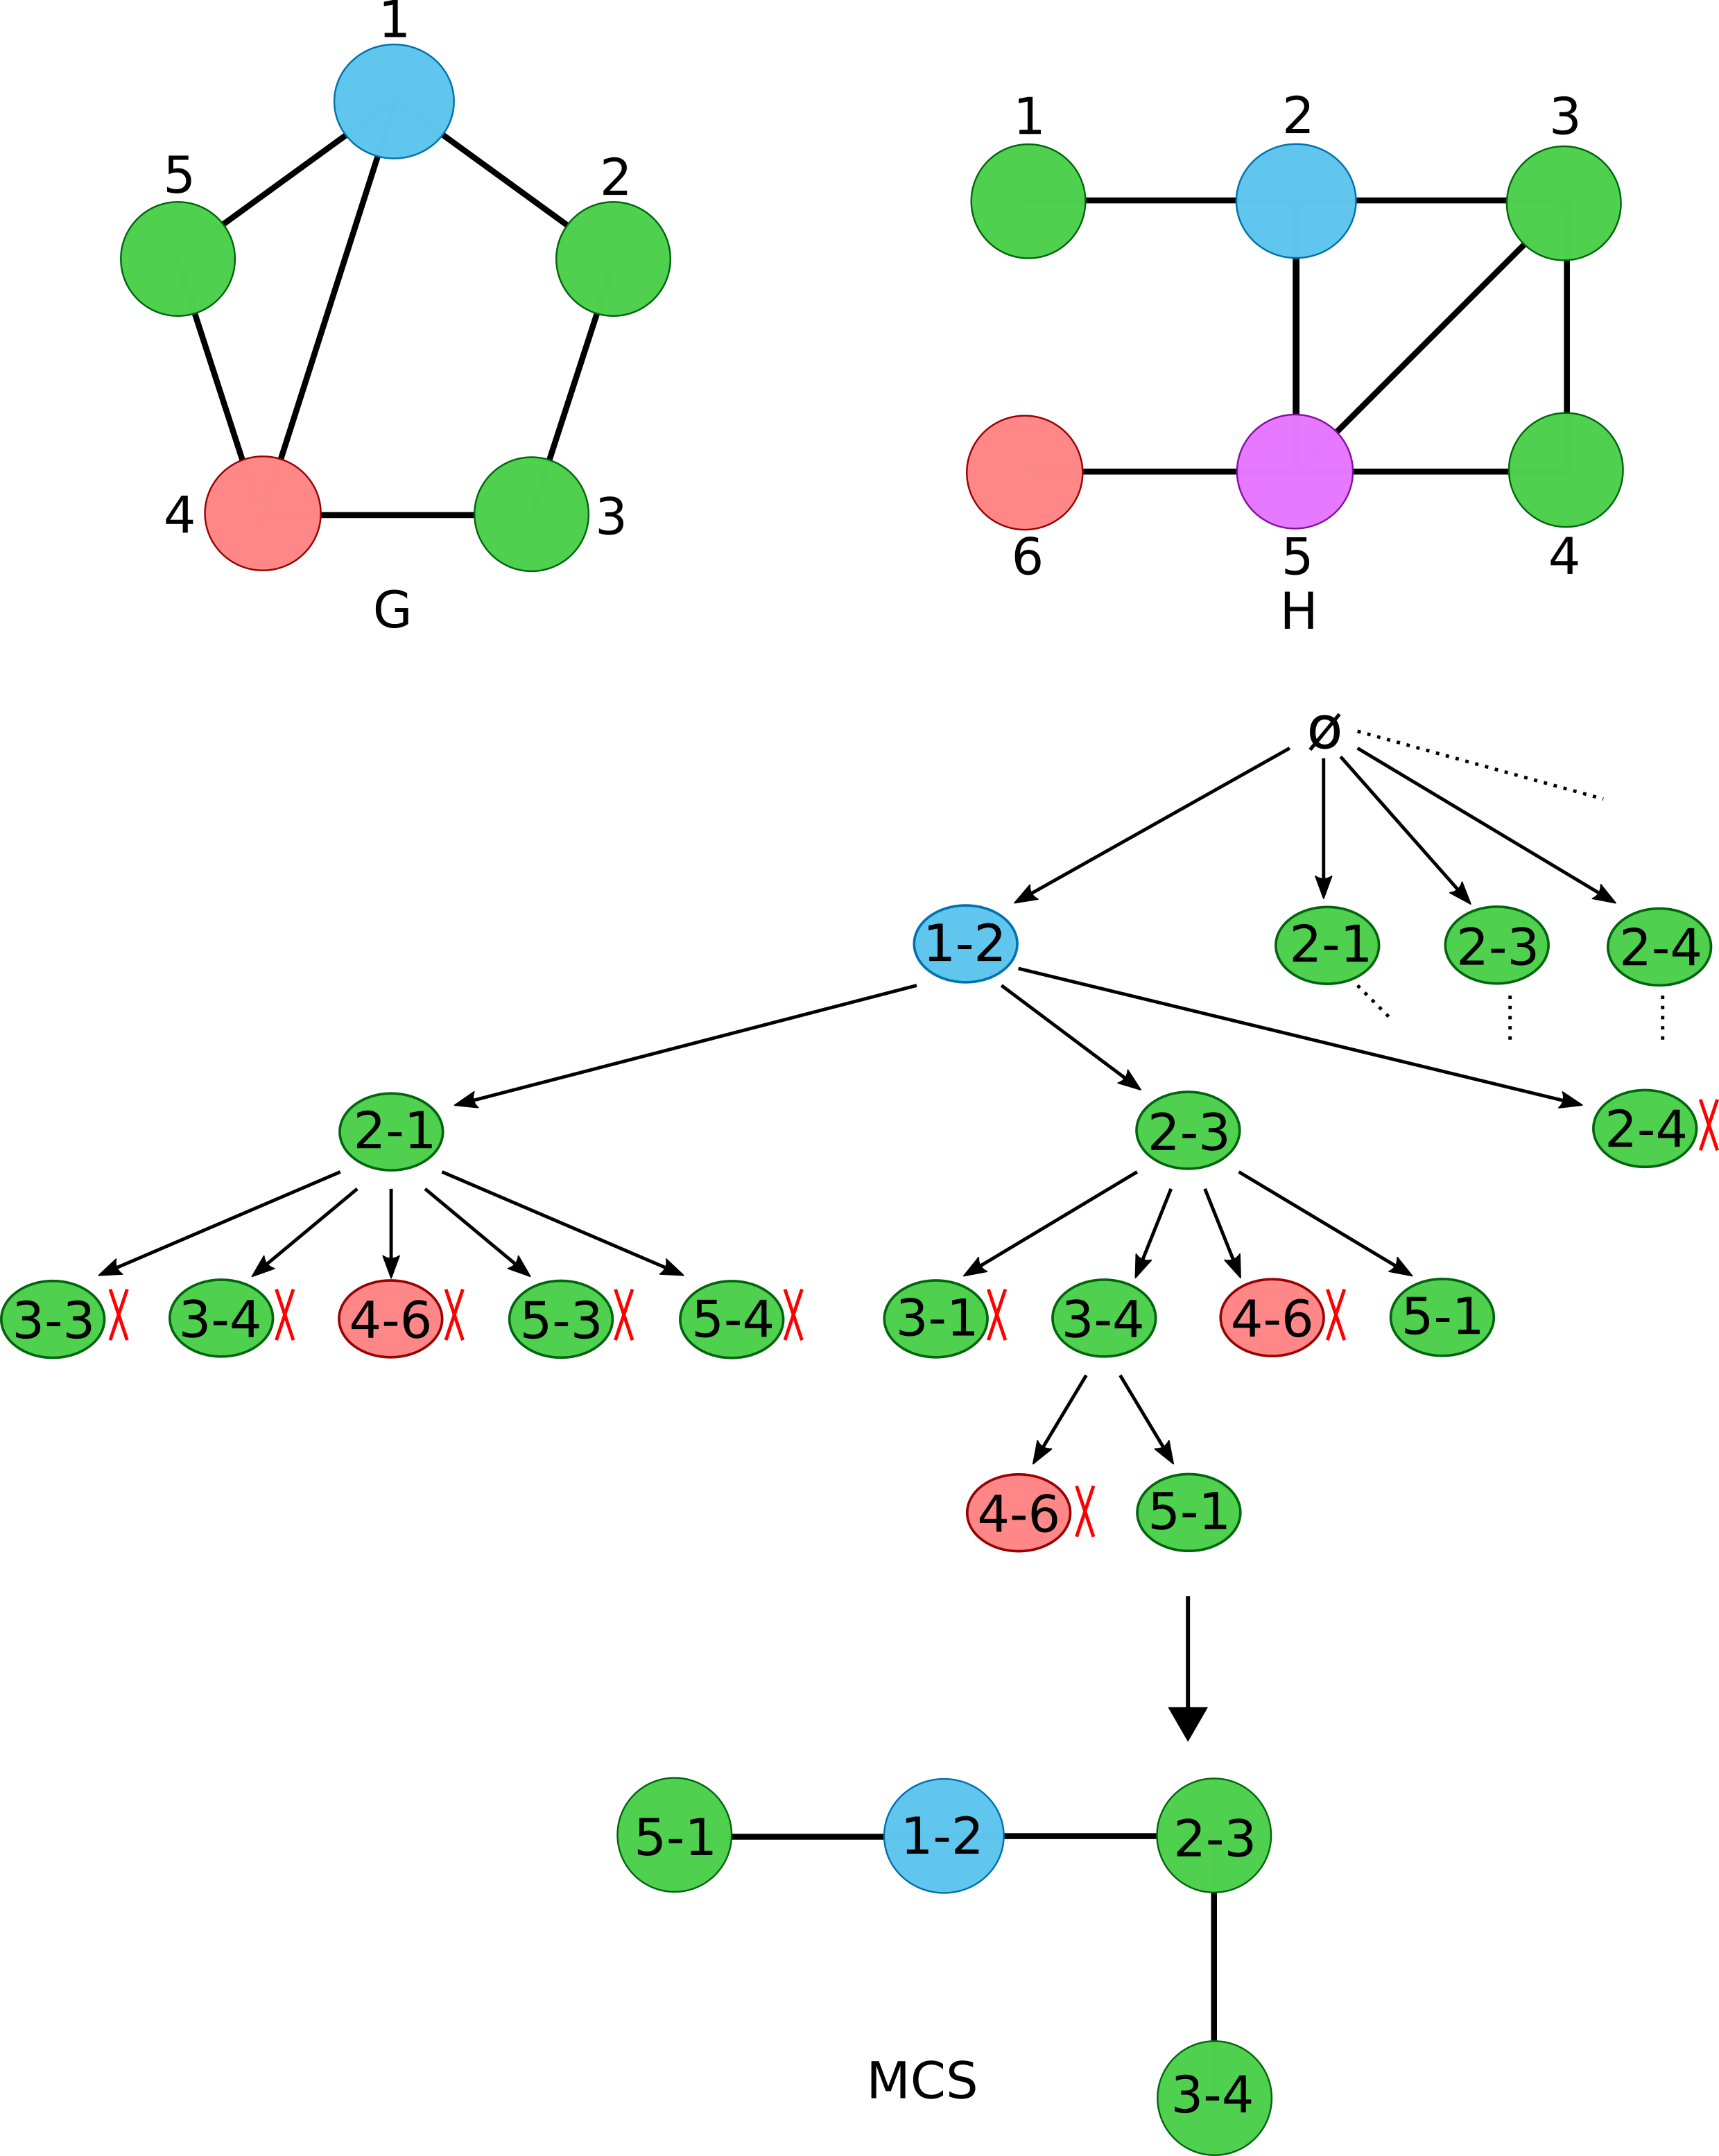
\includegraphics[width=400px]{Figures/s2m/MCS-SI/backtracking_solve.png}
    \caption{\label{backtracking_solve}Exemple de résolution de MCS par un backtracking naïf.
    L'arbre part d'une bijection vide et ajoute un couple à chaque étape.
    Parfois l'algorithme tombe sur un couple compatible mais dont les voisins ne sont pas présents dans la bijection.
    La solution est alors rejetée (croix rouge).
    La solution est trouvée par l'ensemble des chemins qui mènent aux feuilles valides les plus profondes dans l'arbre.}
  \end{center}
\end{figure}


\textbf{Recherche par Backtracking}~~~
La majorité des algorithmes exacts effectuent des recherches via des méthodes de backtracking~\cite{manic_branch&cut_2009,mcgregor_backtrack_1982,kawabata_build-up_2011}.
Un MCS est une bijection entre deux sous-ensembles de n\oe{}uds dans deux graphes distincts.
Les méthodes de backtrack effectuent une reconstruction itérative de cette bijection.
Les couples de n\oe{}uds compatibles, n'étant pas encore présents au sein de la bijection, sont ajoutés un à un (voir figure \ref{backtracking_solve}).
Lorsque l'algorithme arrive dans une impasse (plus aucune possibilité d'ajouter un couple), il revient en arrière sur une association puis fait un choix différent.
En sauvegardant l'ensemble qui a contenu le plus de n\oe{}uds, on obtient la clique maximale après le parcours de tout l'arbre des possibilités.
Encore une fois, certaines des techniques citées permettent des accélérations pratiques en coupant des branches de recherche mais jamais l'ordre de grandeur de la complexité n'est changé.
Dans le cas des MCCS, il faut inclure une contrainte supplémentaire~\cite{chang_moderately_2014}.
Chacun des n\oe{}uds du couple à ajouter doit être voisin de l'un des n\oe{}uds d'un même couple précédemment inclus dans la bijection.

Il existe bien d'autres méthodes exactes pour résoudre des MCS pour des graphes particuliers (par exemple pour des quasi-arbres de \textit{treewidth} borné~\cite{yamaguchi_finding_2004}).
Cependant, si nous souhaitons traiter n'importe quelles molécules, même avec les structures les plus extrêmes, nous ne pouvons utiliser ces méthodes.
Nous ne détaillerons donc pas celles-ci ici.


\subsubsection{Les méthodes heuristiques}

Il existe une très grande quantité d'heuristiques de résolution du MCS.
La méthode la plus utilisée est une méthode de recherche par similarités locales~\cite{yan_substructure_2005,willett_similarity_2011}.
Ces heuristiques sont utilisées au sein de bases de données pour rechercher des structures chimiques par ressemblance avec une requête.
Chaque molécule de la base est décomposée en un grand nombre de critères topologiques locaux (l'arité des noeuds par exemple).
Ces critères sont entrés dans un vecteur appelé fingerprint.
Lors d'une requête, le motif recherché est à son tour transformé en \textit{fingerprint} et une mesure de similarité est effectuée avec les vecteurs présents en base.
Les \textit{fingerprints} les ``plus proches'' (d'après une fonction de score~\cite{maggiora_molecular_2011,ndiaye_cp_2011}) sont déclarés contenir une sous partie commune.
Cette méthode ne donne aucune assurance quant à l'obtention de réels MCS.
C'est la rapidité d'exécution de l'algorithme qui est recherchée.
Dans notre cas, cette méthode est inappropriée puisque nous cherchons des MCS exacts.

D'autres méthodes se rapprochent plus des méthodes exactes par recherche backtracking~\cite{grosso_simple_2008, wang_fmcsr:_2013}.
Ici, les auteurs construisent plusieurs bijections en parallèle.
La différence avec les méthodes exactes est qu'ils ne reviennent jamais sur les décisions prises pour construire les MCS.
Un nombre fixe de bijections est maintenu en permanence.
Ces bijections ont été sélectionnées par une fonction de score comme étant celles qui avaient le plus de chance de mener à un MCS.
Au final, les bijections trouvées ne seront pas forcément les vrais MCS.
Cette seconde méthode est très intéressante lorsque l'on cherche un bon rapport entre rapidité et qualité du résultat.


\subsection{Isomorphisme de sous-graphe}

\label{SI_p}

\subsubsection{Définition}

\begin{figure}[!ht]
  \begin{center}
    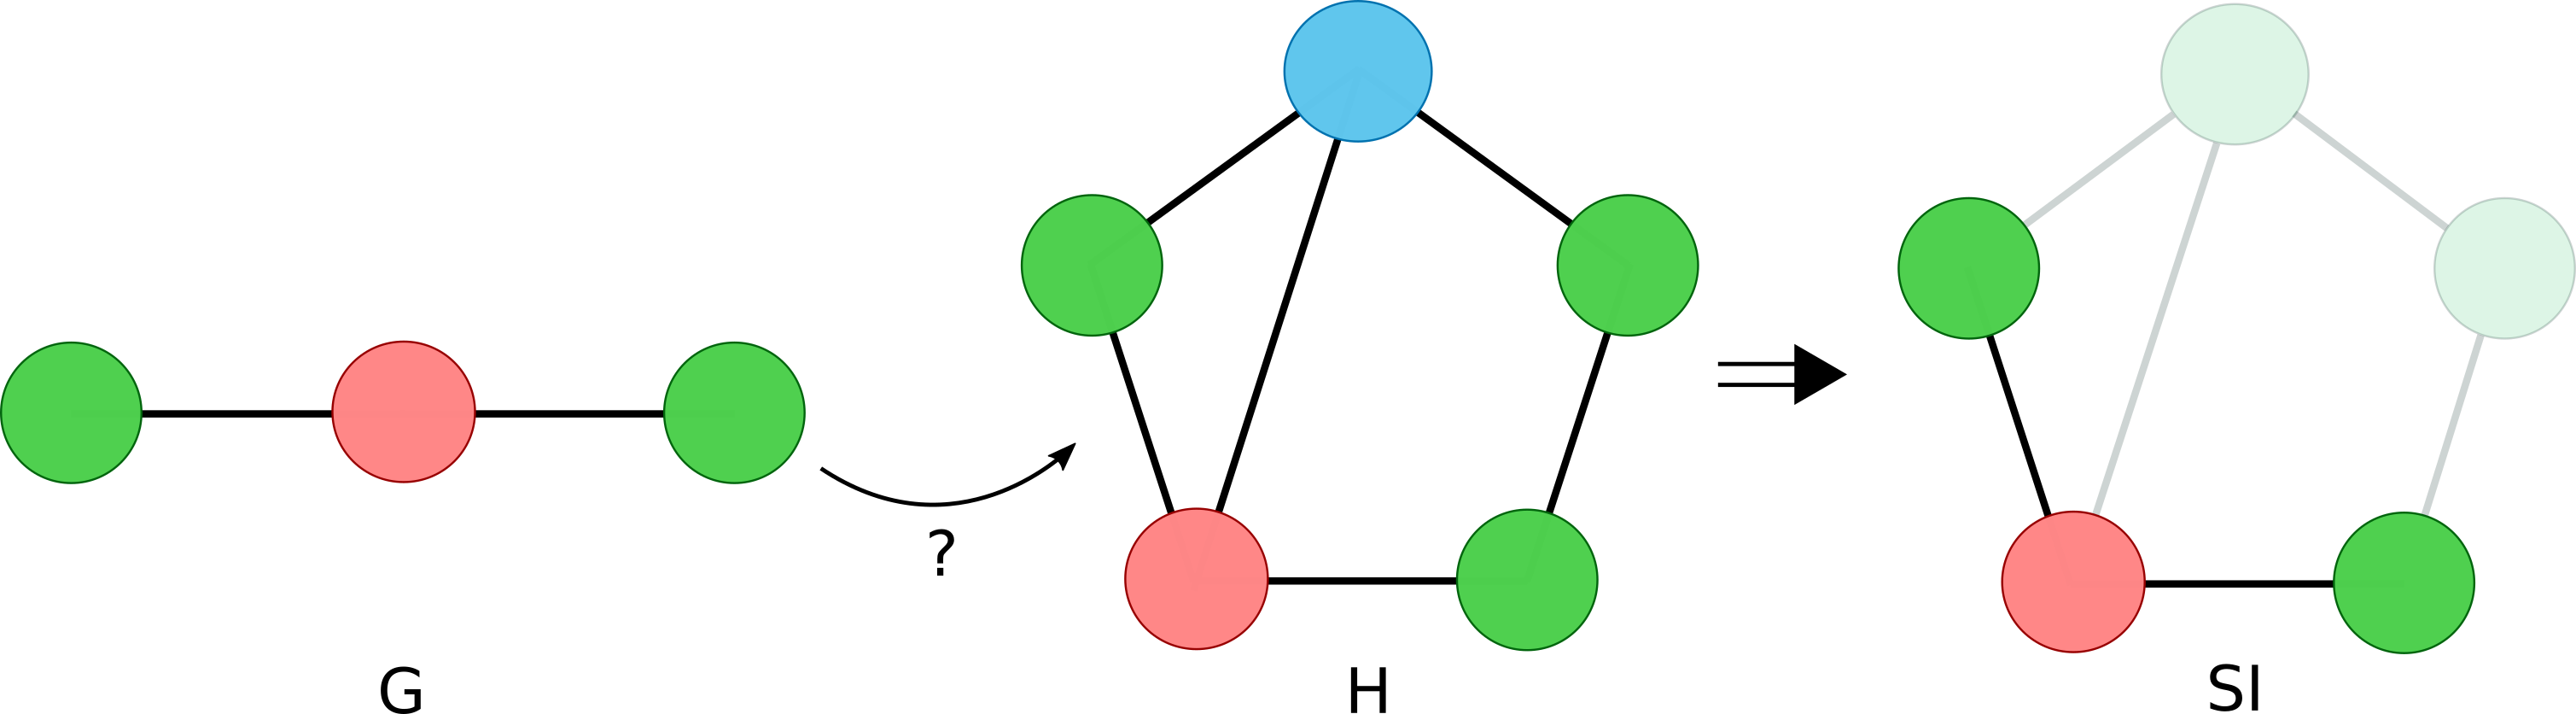
\includegraphics[width=450px]{Figures/s2m/MCS-SI/si.png}
    \caption{\label{SI_fig}SI obtenu à partir de la recherche du graphe G dans H.
    Sur cet exemple, il n'y a qu'une seule possibilité mais si nous avions cherché une chaîne comme Vert-Rouge-Bleu, nous aurions eu deux SI différents.}
  \end{center}
\end{figure}

Définissions à son tour le problème d'isormorphisme de sous-graphe (Subgraph Isomorphism (SI)).
Comme le nom l'indique, le problème SI est un problème de recherche d'un graphe dans une sous partie d'un autre.
C'est à dire que G est sous-graphe de H lorsque tous les n\oe{}uds et toutes les arêtes de G sont retrouvées structurées de la même manière dans H (voir figure \ref{SI_fig}).
Tout comme le MCS, le problème du SI a été prouvé NP-Complet~\cite{garey_computers_1979}.

Pour notre problème, nous pouvons à nouveau effectuer une réduction vers le problème SI, puis résoudre ce problème par des algorithmes déjà publiés.
Nous souhaitons rechercher des monomères au sein de peptides, ce qui reviendrait à chercher plusieurs fois un petit graphe atomique monomérique dans un gros graphe atomique peptidique.

Les méthodes de résolution actuelles sont toutes très similaires et dérivent d'une même technique de backtracking.
La plupart de ces méthodes sont des résolutions exactes.
Bien que NP-complet, ces algorithmes restent très praticables pour des graphes étiquetés, lorsqu'on ne recherche pas au sein de graphes répétitifs (qui sont constitués de multiples répétitions d'un même morceau).
Voyons ensemble plusieurs algorithmes représentatifs.


\subsubsection{L'algorithme de Ullman}

\begin{figure}[!ht]
  \begin{center}
    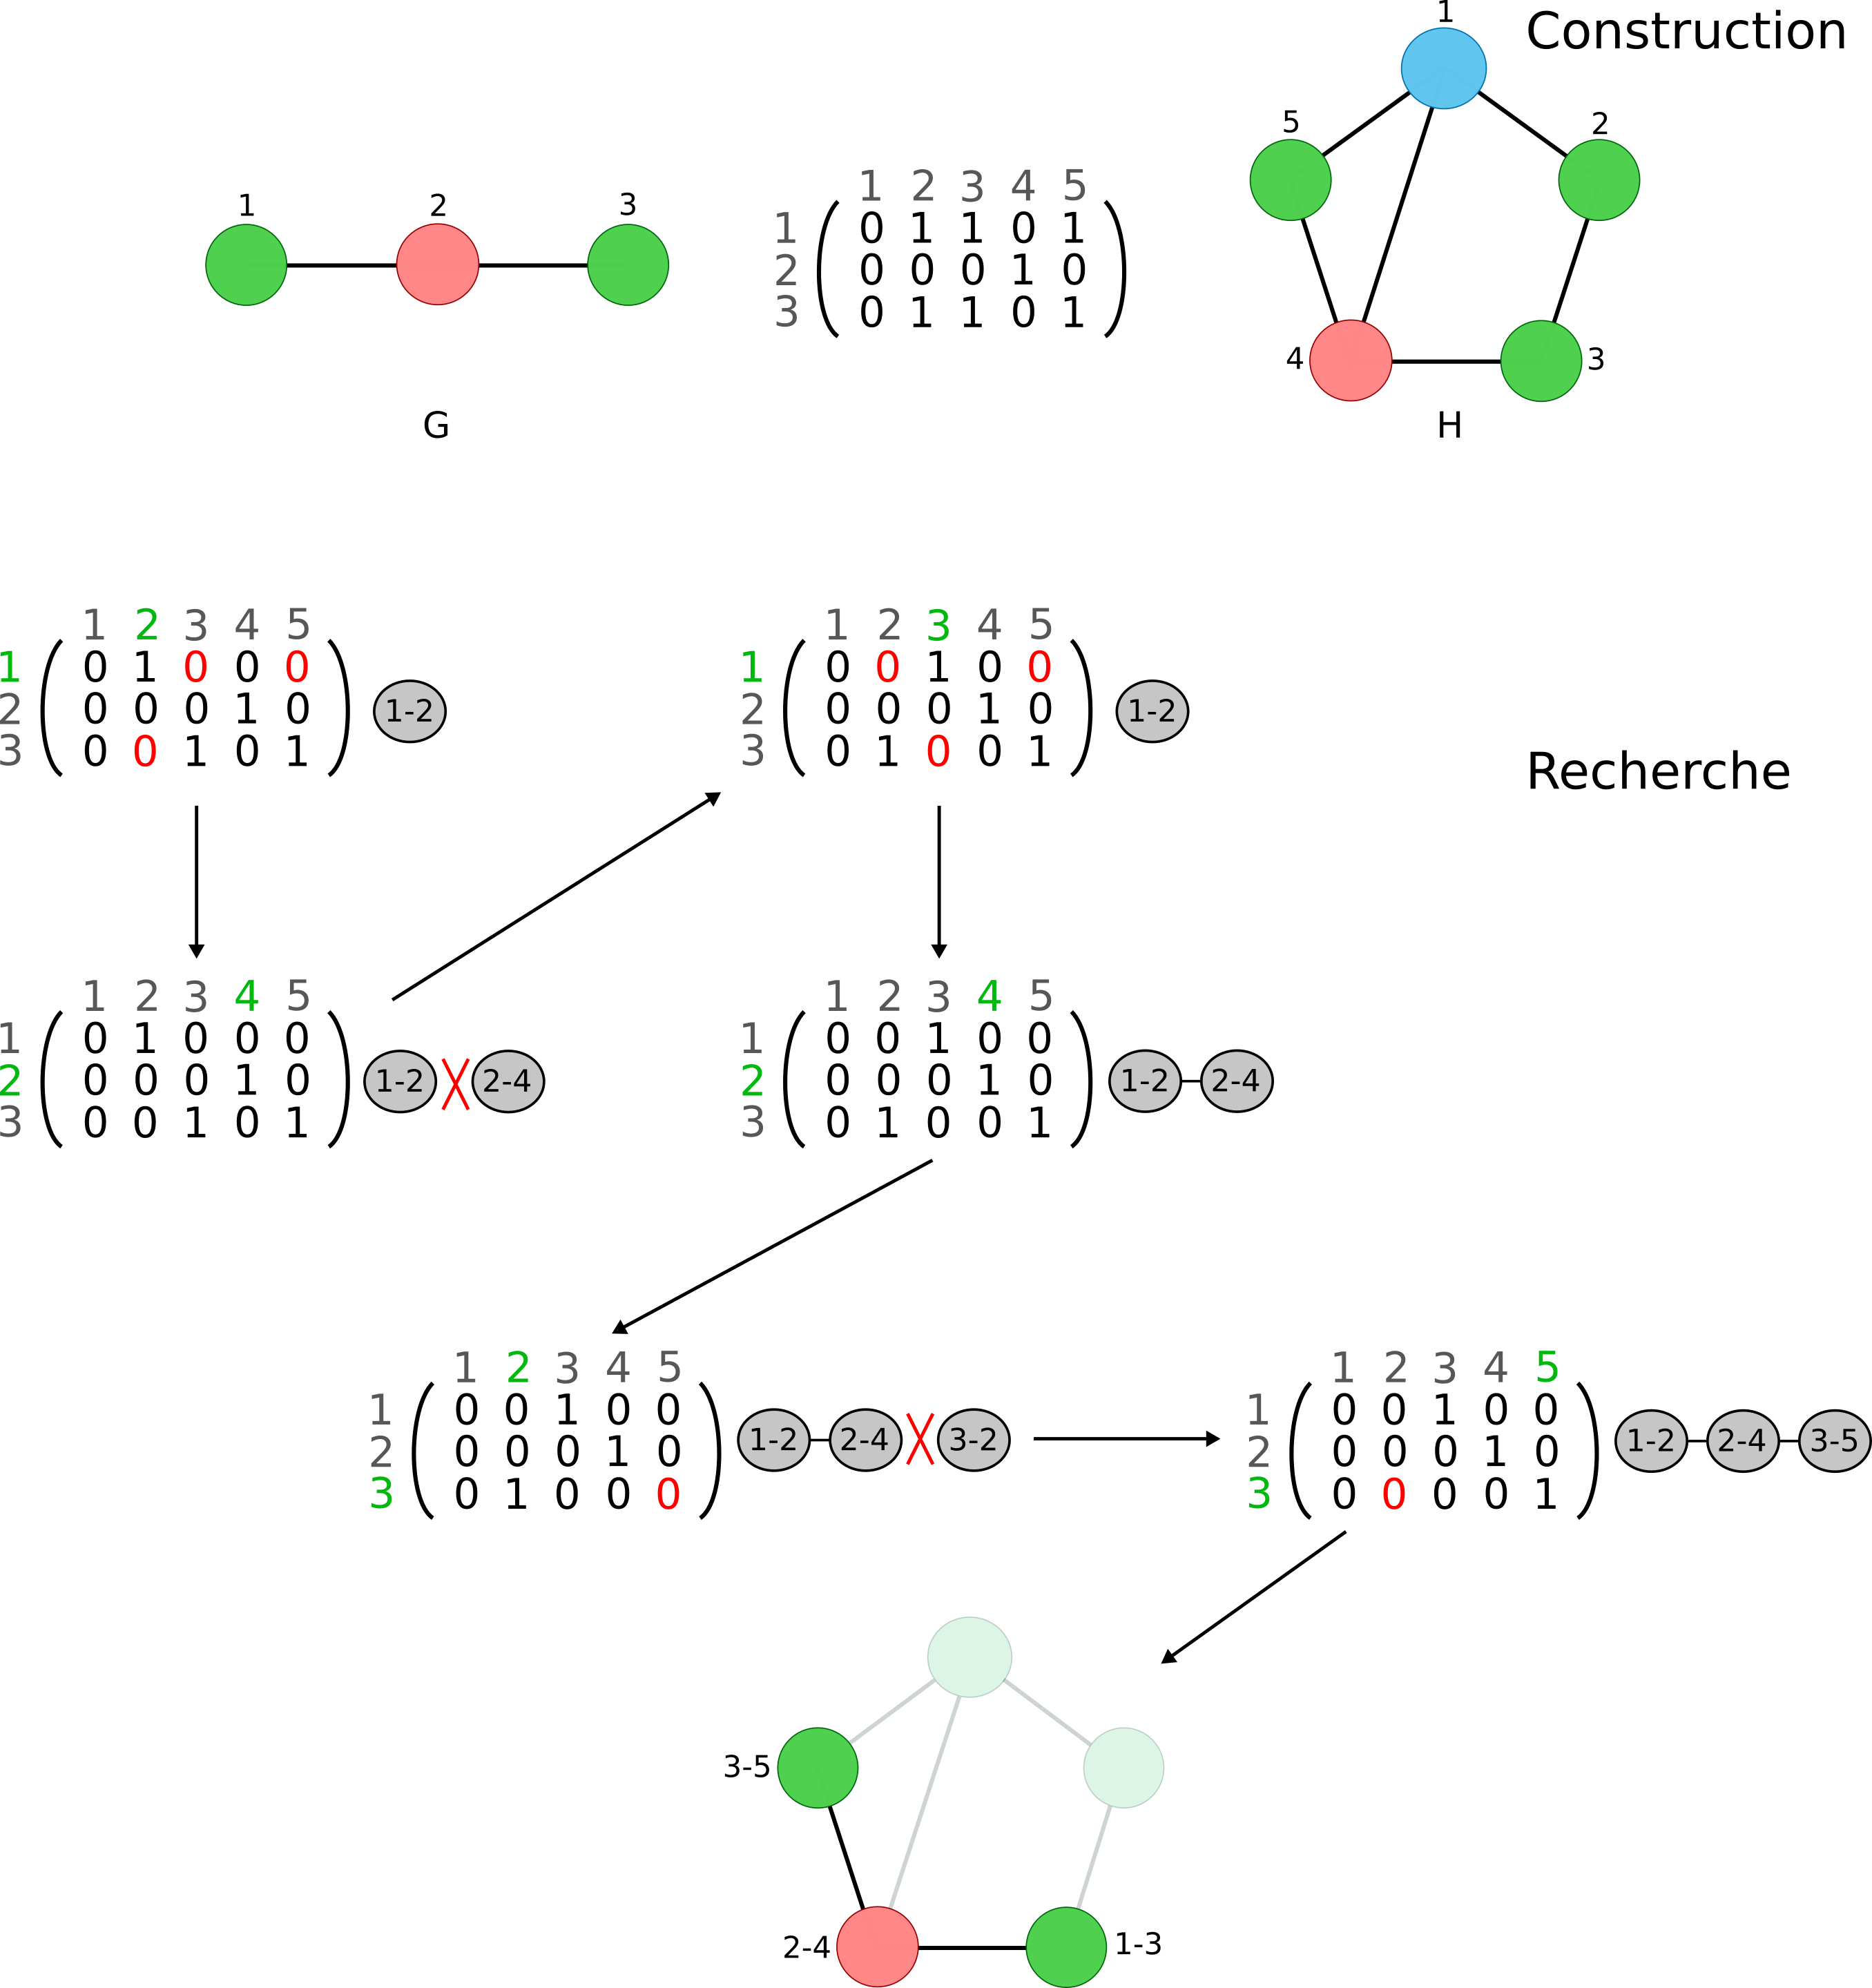
\includegraphics[width=450px]{Figures/s2m/MCS-SI/ullman.png}
    \caption{\label{ullman_fig}Recherche d'un isomorphisme de sous-graphe par l'algorithme d'Ullman.
    Dans la partie ``construction'', vous pouvez voir la matrice créée à partir des graphes G et H.
    Dans la partie ``recherche'' sont présentées les étapes successives de création d'un SI (voir texte pour détail).
    Si nous avions voulu obtenir tous les isomorphismes (et pas juste un seul), il aurait fallu continuer le backtracking jusqu'au bout.}
  \end{center}
\end{figure}

L'algorithme de Ullman est l'un des premiers à avoir été proposé dans les années 70~\cite{ullmann_algorithm_1976}.
Certaines de ses variantes sont toujours utilisées dans certaines librairies telles que Openbabel~\cite{oboyle_open_2011}.
L'algorithme se base sur la matrice de compatibilité entre les graphes (voir figure \ref{ullman_fig}).
Une matrice de compatibilité est une matrice dont chaque ligne représente un n\oe{}ud de G et chaque colonne un n\oe{}ud de H.
Soient $g$ et $h$ correspondants respectivement à un n\oe{}ud du graphe G et du graphe H.
Soient $i$ et $j$ les numéros des lignes et colonnes de la matrice correspondants à $g$ et $h$.
La case de coordonnées $(i,j)$ contient un 1 si $g$ et $h$ ont une étiquette compatible et que l'arrité de $h$ est suppérieure ou égale à l'arrité de $g$.
Pour obtenir un SI à partir de cette matrice, il faut retirer des 1 de la matrice jusqu'à en obtenir un seul 1 par ligne.
A chaque étape, un n\oe{}ud $g$ de G est choisi pour continuer l'isomorphisme.
Ce n\oe{}ud correspond à une ligne $i$.
Puis une colonne $j$ est choisie de telle manière à ce que la case $(i,j)$ de la matrice contienne un 1.
Le couple $(i,j)$ nous donne le couple $(g,h)$ qui peut être ajouter à l'isomorphisme.
Avant cet ajout, il faut également vérifier que tous les voisins de $h$ correspondent bien aux voisins de $g$ (condition non respectée à l'étape 2 et 5 de la partie recherche du schéma).
Puisque nous ajoutons ce couple à l'isomorphisme, il faut remplacer tous les 1 de la ligne et la colonne choisies par des 0 (excepté pour la case $(i,j)$).
À ce moment, si au moins une ligne a été vidée de tous ses 1, c'est que l'isomorphisme n'est pas possible et il faut revenir à l'étape précédente.
L'algorithme continue récursivement jusqu'à obtenir un 1 par ligne ou ne trouver aucun isomorphisme.
En choisissant bien les lignes et les colonnes par lesquelles l'algorithme commence (par exemple celles pour lesquelles il n'y pas de doute), on arrive à obtenir des temps d'exécution très courts pour la recherche d'un SI.
Cependant, pour obtenir tous les SI, il faut parcourir tout l'arbre des possibles, ce qui ralentit l'algorithme.


\subsubsection{VF2, un algorithme de backtracking classique}

Tout comme pour le MCS, le SI peut être résolu par un backtracking classique par association de n\oe{}uds deux à deux.
C'est la méthode majoritairement utilisée puisqu'elle fonctionne très bien en pratique.
Contrairement à l'algorithme d'Ullman qui nécessite d'effectuer des opérations sur des matrices potentiellement très grandes, la méthode par backtracking classique n'a pas besoin de grands espaces mémoire.
L'algorithme VF2~\cite{cordella_subgraph_2004} utilisent ce principe.
Les SI se forment par ajouts successifs de couples de n\oe{}uds compatibles avec retour en arrière s'il n'est plus possible d'avoir un couple.
VF2 est un algorithme de recherche de SI pour des graphes non orientés et non étiquetés.

% 
%   \begin{algorithm}[H]
%     \caption{Algorithme VF2 pour graphes non étiquetés}
%     \KwData{Un graphe $G(V,E)$ et un graphe $H(V',E')$ avec $|V| \leq |V'|$ et $s$ un état contenant les mappings déjà effectués
%     entre les deux graphes}
%     \KwResult{Un mapping entre les éléments de $V$ et une sous partie des éléments de $V'$ telle que $H$ soit un isomorphisme de
%     sous-graphe de $H$}
%     
%     \uIf {$s$ contient un mapping de tous les éléments de $V$} {
%       \KwRet $Mapping(s)$\;
%     } \uElse {
%       \uIf {$Mapping(s)$ est vide} {
% 	$P \gets$ ensemble des $p(x,y)$ tq $x \in V$ et $y \in V'$ \;
%       } \uElse {
% 	$P \gets$ ensemble des $p(x,y)$ tq $x \in V$, $y \in V'$ et $\exists p(a,b) \in Mapping(s)$ tq $a$ et $x$ soient voisins dans
% 	$G$ et $b$, $y$ voisins dans $H$ \;
%       }
%       
%       \For {$p \in P$} {
% 	$s' \gets p \cup s$\;
% 	\If {$VF2(G, H, s') != \emptyset$} {\KwRet $Mapping(s')$\;}
%       }
%       
%       \KwRet $\emptyset$ \;
%     }
%   \end{algorithm}

\begin{figure}[!ht]
  \begin{center}
    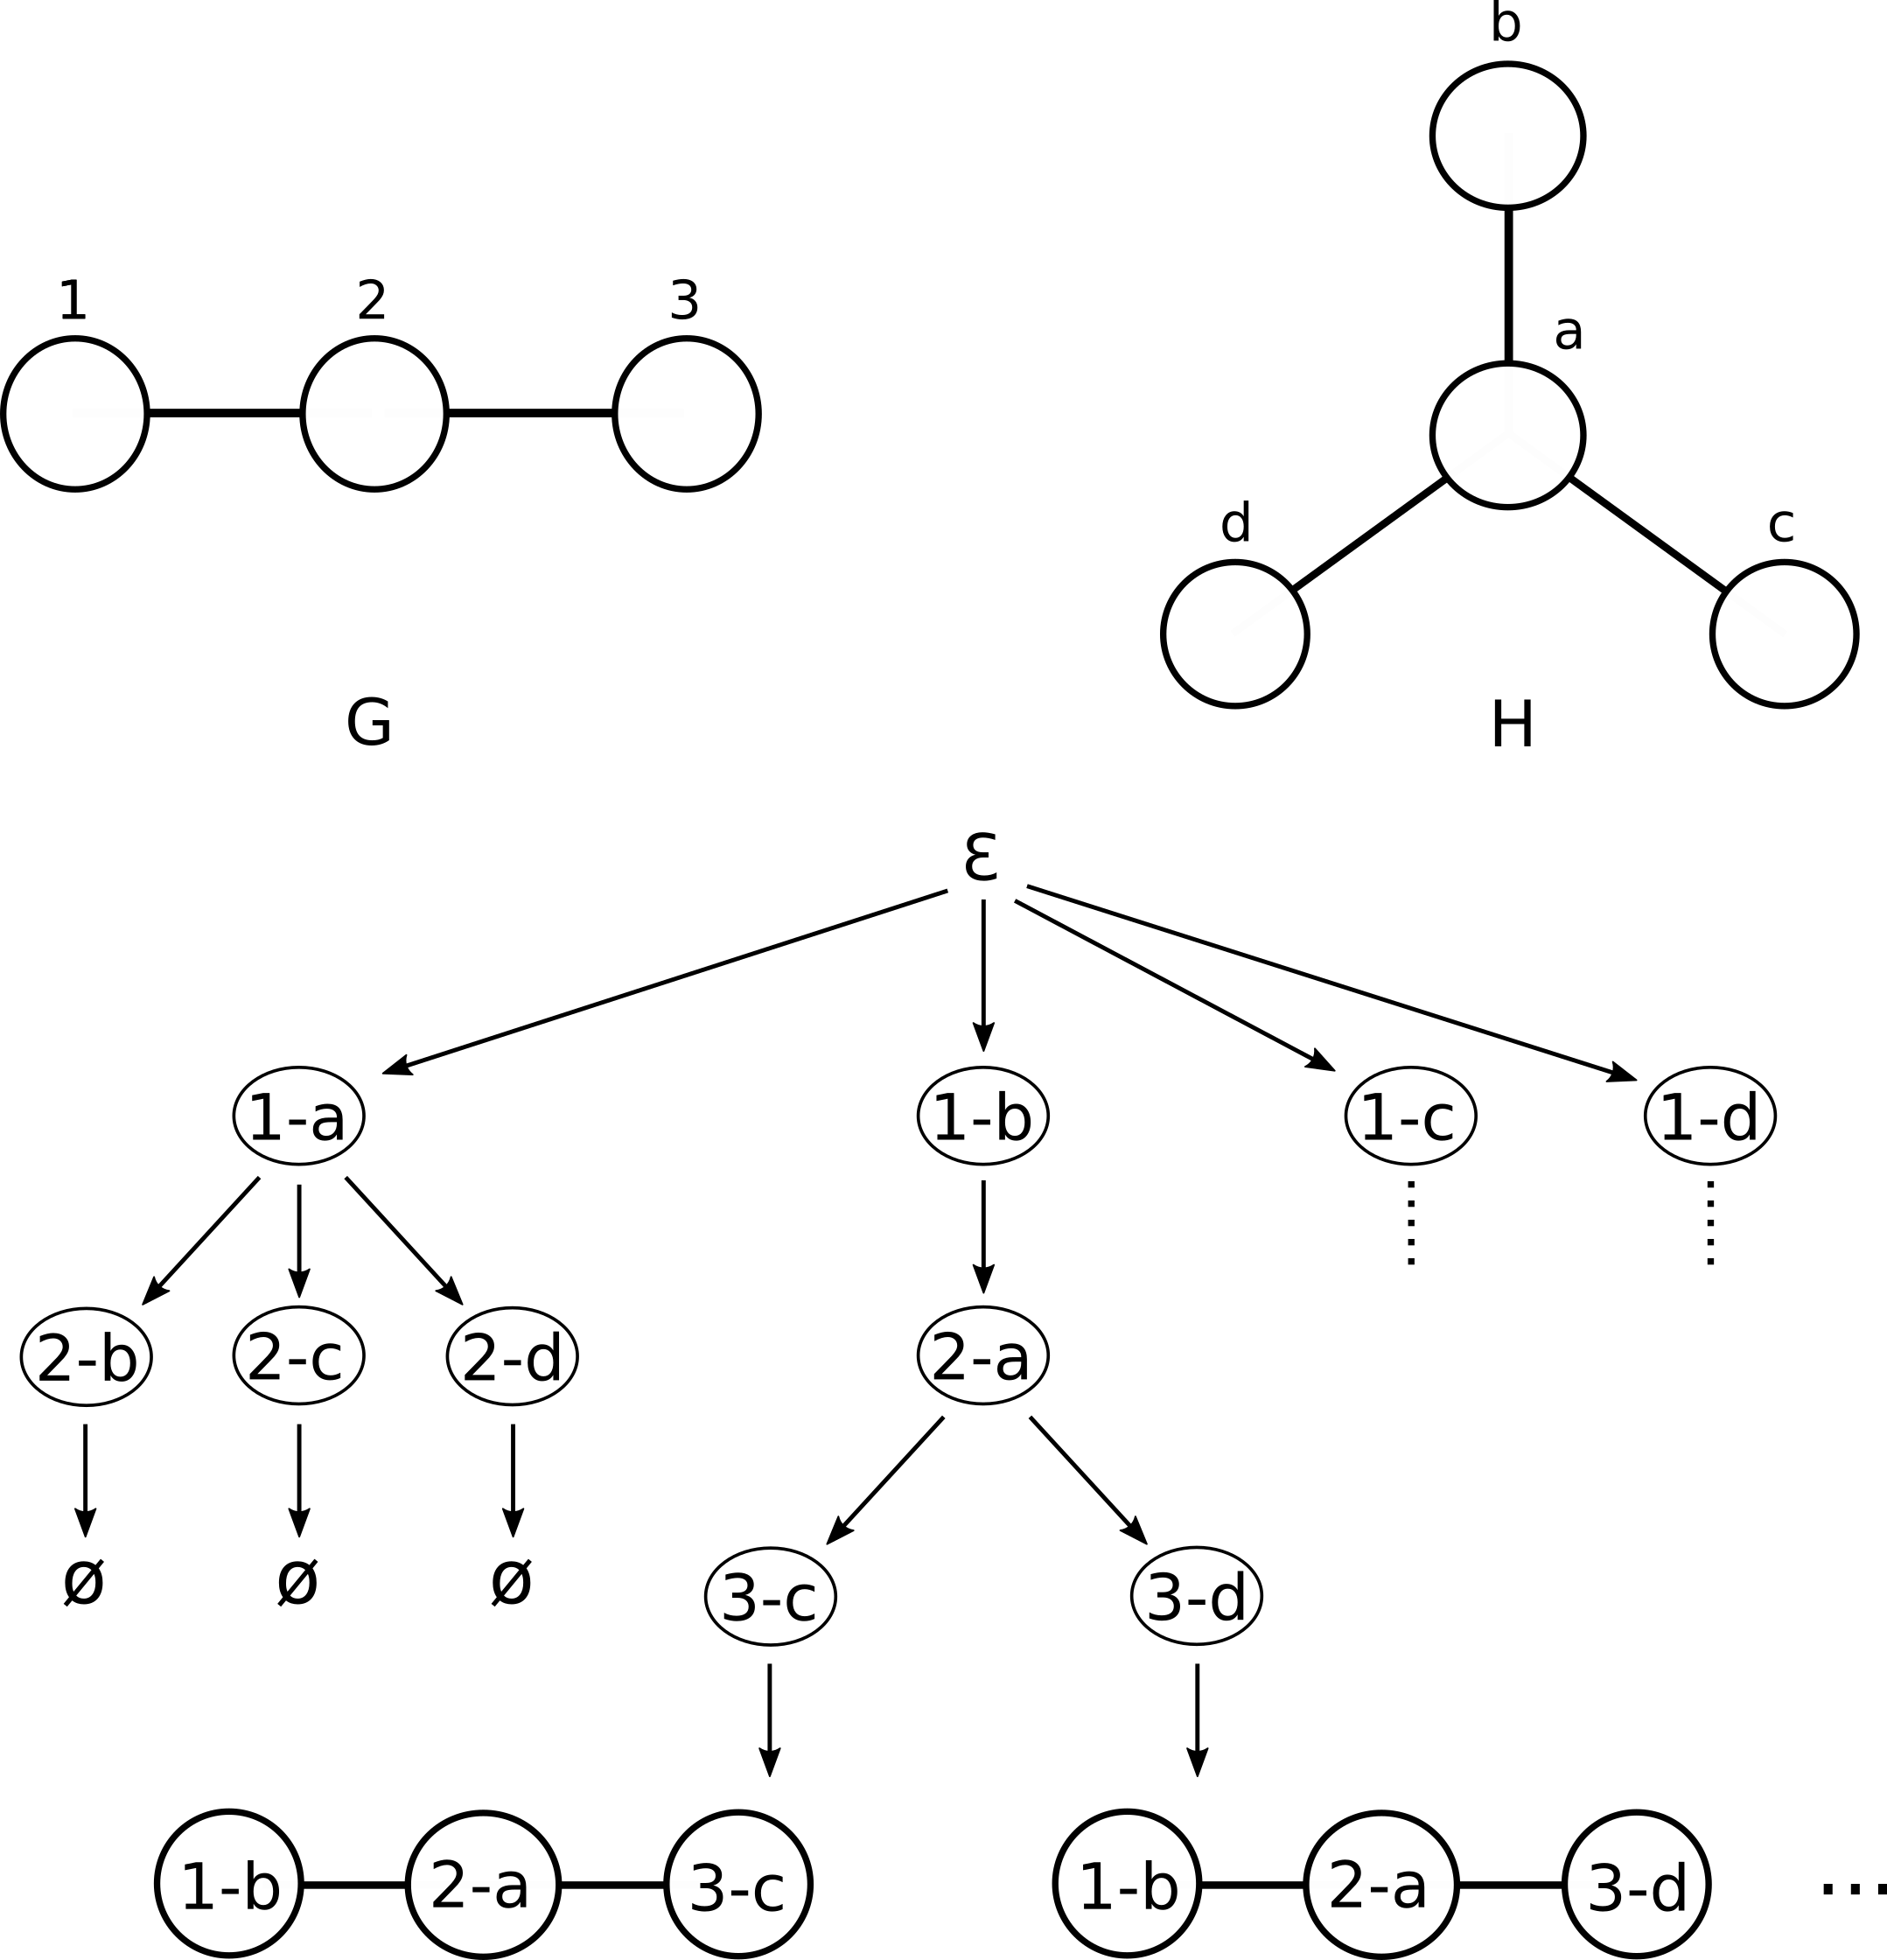
\includegraphics[width=350px]{Figures/s2m/recherche/VF2.png}
    \caption{\label{vf2}Backtracking de VF2 pour extraire l'ensemble de tous les SI possibles.}
  \end{center}
\end{figure}

Expliquons cet algorithme en utilisant le schéma \ref{vf2}.
A la première étape, nous nous trouvons avec un ensemble vide de n\oe{}uds couplés de $G$ et $H$.
Nous générons donc toutes les possibilités de couples entre tous les n\oe{}uds des deux graphes (Il est à noter que l'algorithme
est décrit de cette façon dans l'article mais qu'il n'est nécessaire de générer que les couples à partir d'un seul n\oe{}ud de $G$
et de l'ensemble des n\oe{}uds de $H$.)
Une fois ces couples créés, nous les parcourons tous en appelant récursivement la fonction.
Dans l'exemple, le premier appel récursif est effectué après avoir assemblé '1' à 'a'.
Cette voie est sans issue car quel que soit l'assemblage entre '2' et un n\oe{}ud de $H$, plus aucun couple de voisins ne pourra être
généré.
En effet, pour générer l'ensemble $P$, il est nécessaire de regarder tous les voisins de 'b' alors que le n\oe{}ud ne possède plus
de voisins hors de $s$.
Une fois toutes les tentatives échouées, l'algorithme remonte dans l'arbre et change l'association '1'-'a' pour l'association
'1'-'b'.
Récursivement, l'algorithme conclut à un isomorphisme {(1,b);(2,a);(3,c)}.

En l'état, l'algorithme VF2 ne reconnaît qu'un seul et unique isomorphisme.
On peut modifier simplement l'algorithme afin de récupérer tous les isomorphismes en ne retournant pas une fois que l'un d'eux est
trouvé mais en l'enregistrant dans un ensemble puis en continuant l'exploration de l'arbre jusqu'au bout.
Puisque que tout l'arbre est exploré à chaque recherche, l'algorithme est exponentiel.
Pour être plus précis il est en $O(n^m)$, donc non calculable dans les pires des cas ($n$ taille de G et $m$ de H).

Cet algorithme est très pratique pour trouver un SI, mais pas pour les trouver tous.
En pratique, il est utilisé au sein de grandes librairies logicielles de chimie comme CDK~\cite{steinbeck_chemistry_2003} pour faire des requêtes par structure sur des ensembles chimiques.


\subsubsection{D'autres algorithmes de SI}

Contrairement à la recherche de MCS, il n'existe pas beaucoup d'alternatives heuristiques pour le SI.
Ceci peut s'expliquer par le fait que des algorithmes exacts et praticables existent pour trouver les SI.
De plus, les heuristiques de MCS permettent d'obtenir des résultats de SI en ajoutant des contraintes (Le SI étant un cas particulier du MCS).
Dans tous les cas, ces heuristiques de SI sont des dérivés de la technique par backtracking~\cite{kaijar_developing_2012}.
Ces algorithmes essaient en supplément d'éviter l'exploration de toutes les branches par de la sélection des plus ``prometteuses''.
Par exemple, on préférera explorer des isomorphismes commençant par des paires de noeuds d'arité forte car ils sont un fort indice de ``bon isomorphisme''.

Il existe également de nombreux algorithmes pour des cas particuliers de SI.
Par exemple, il est possible de résoudre le problème SI en temps polynomial pour des arbres~\cite{shamir_faster_1997}, des graphes planaires~\cite{eppstein_subgraph_1995,dorn_planar_2009} ou des graphes de \textit{treewidth} faible~\cite{hajiaghayi_subgraph_2007}.
Dans tous les cas, il est possible de trouver au moins une molécule (pas forcément NRP) ne répondant pas à l'un de ces critères et c'est pour cela que nous avons préféré ne pas les utiliser.


\subsection{Choisir l'algorithme de recherche de monomères}

Pour pouvoir rechercher les monomères, nous devions choisir entre toutes les approches algorithmiques citées ci-dessus.
Premièrement, lorsque nous recherchons un monomère dans un peptide, nous souhaitons connaître tous les endroits où il peut apparaitre.
Nous ne souhaitons donc pas utiliser d'approches heuristiques.
Deuxièmement, le MCS ne paraît pas très pratique dans notre cas.
En effet, les NRP regorgent de monomères proches les uns des autres (variation de un ou deux atomes/liaisons).
Il n'est donc pas facile, lorsque l'on obtient un résultat, de savoir si la molécule trouvée est la bonne ou si c'est le monomère voisin à un atome de distance qui a été détecté.
Enfin, en comparant les algorithmes de recherche exacte de solutions, ceux de résolution de SI sont plus adaptés et rapide en pratique.
Au début, nous ne connaissions pas l'existence de l'algorithme VF2 et aucun des autres algorithmes ne nous convenait en temps de calcul.
De notre côté, nous avons indépendamment redéveloppé un algorithme étendu de VF2 appliqué aux graphes étiquetés et suffisamment rapide pour pouvoir trouver tout SI quasi-instantanément.
La section suivante donnera tous les détails concernant cet algorithme et son intégration à s2m.




\section{Construction de Smiles2Monomers}

\label{algos_s2m}

\subsection{Isomorphisme de sous-graphe appliqué à la recherche de monomères}

\label{isomorphisme_p}

Notre logiciel appelé Smiles2Monomers (s2m), doit débuter par la recherche de l'ensemble des monomères au sein d'un polymère cible.
Comme nous l'avons vu dans l'état de l'art, nous pouvons transformer ce problème en un problème de graphe appelé isomorphisme de sous-graphe (SI).
Dans cette partie, nous allons présenter en détail la variante que nous avons conçu, de l'algorithme de résolution de SI appelé VF2.
Puis nous montrerons en quoi les étiquettes des n\oe{}uds du graphes influencent le temps de calcul afin en déduire une méthode de recherche efficace.

\subsubsection{Notre algorithme pour les graphes étiquetés}


\begin{figure}[!ht]
  \begin{center}
    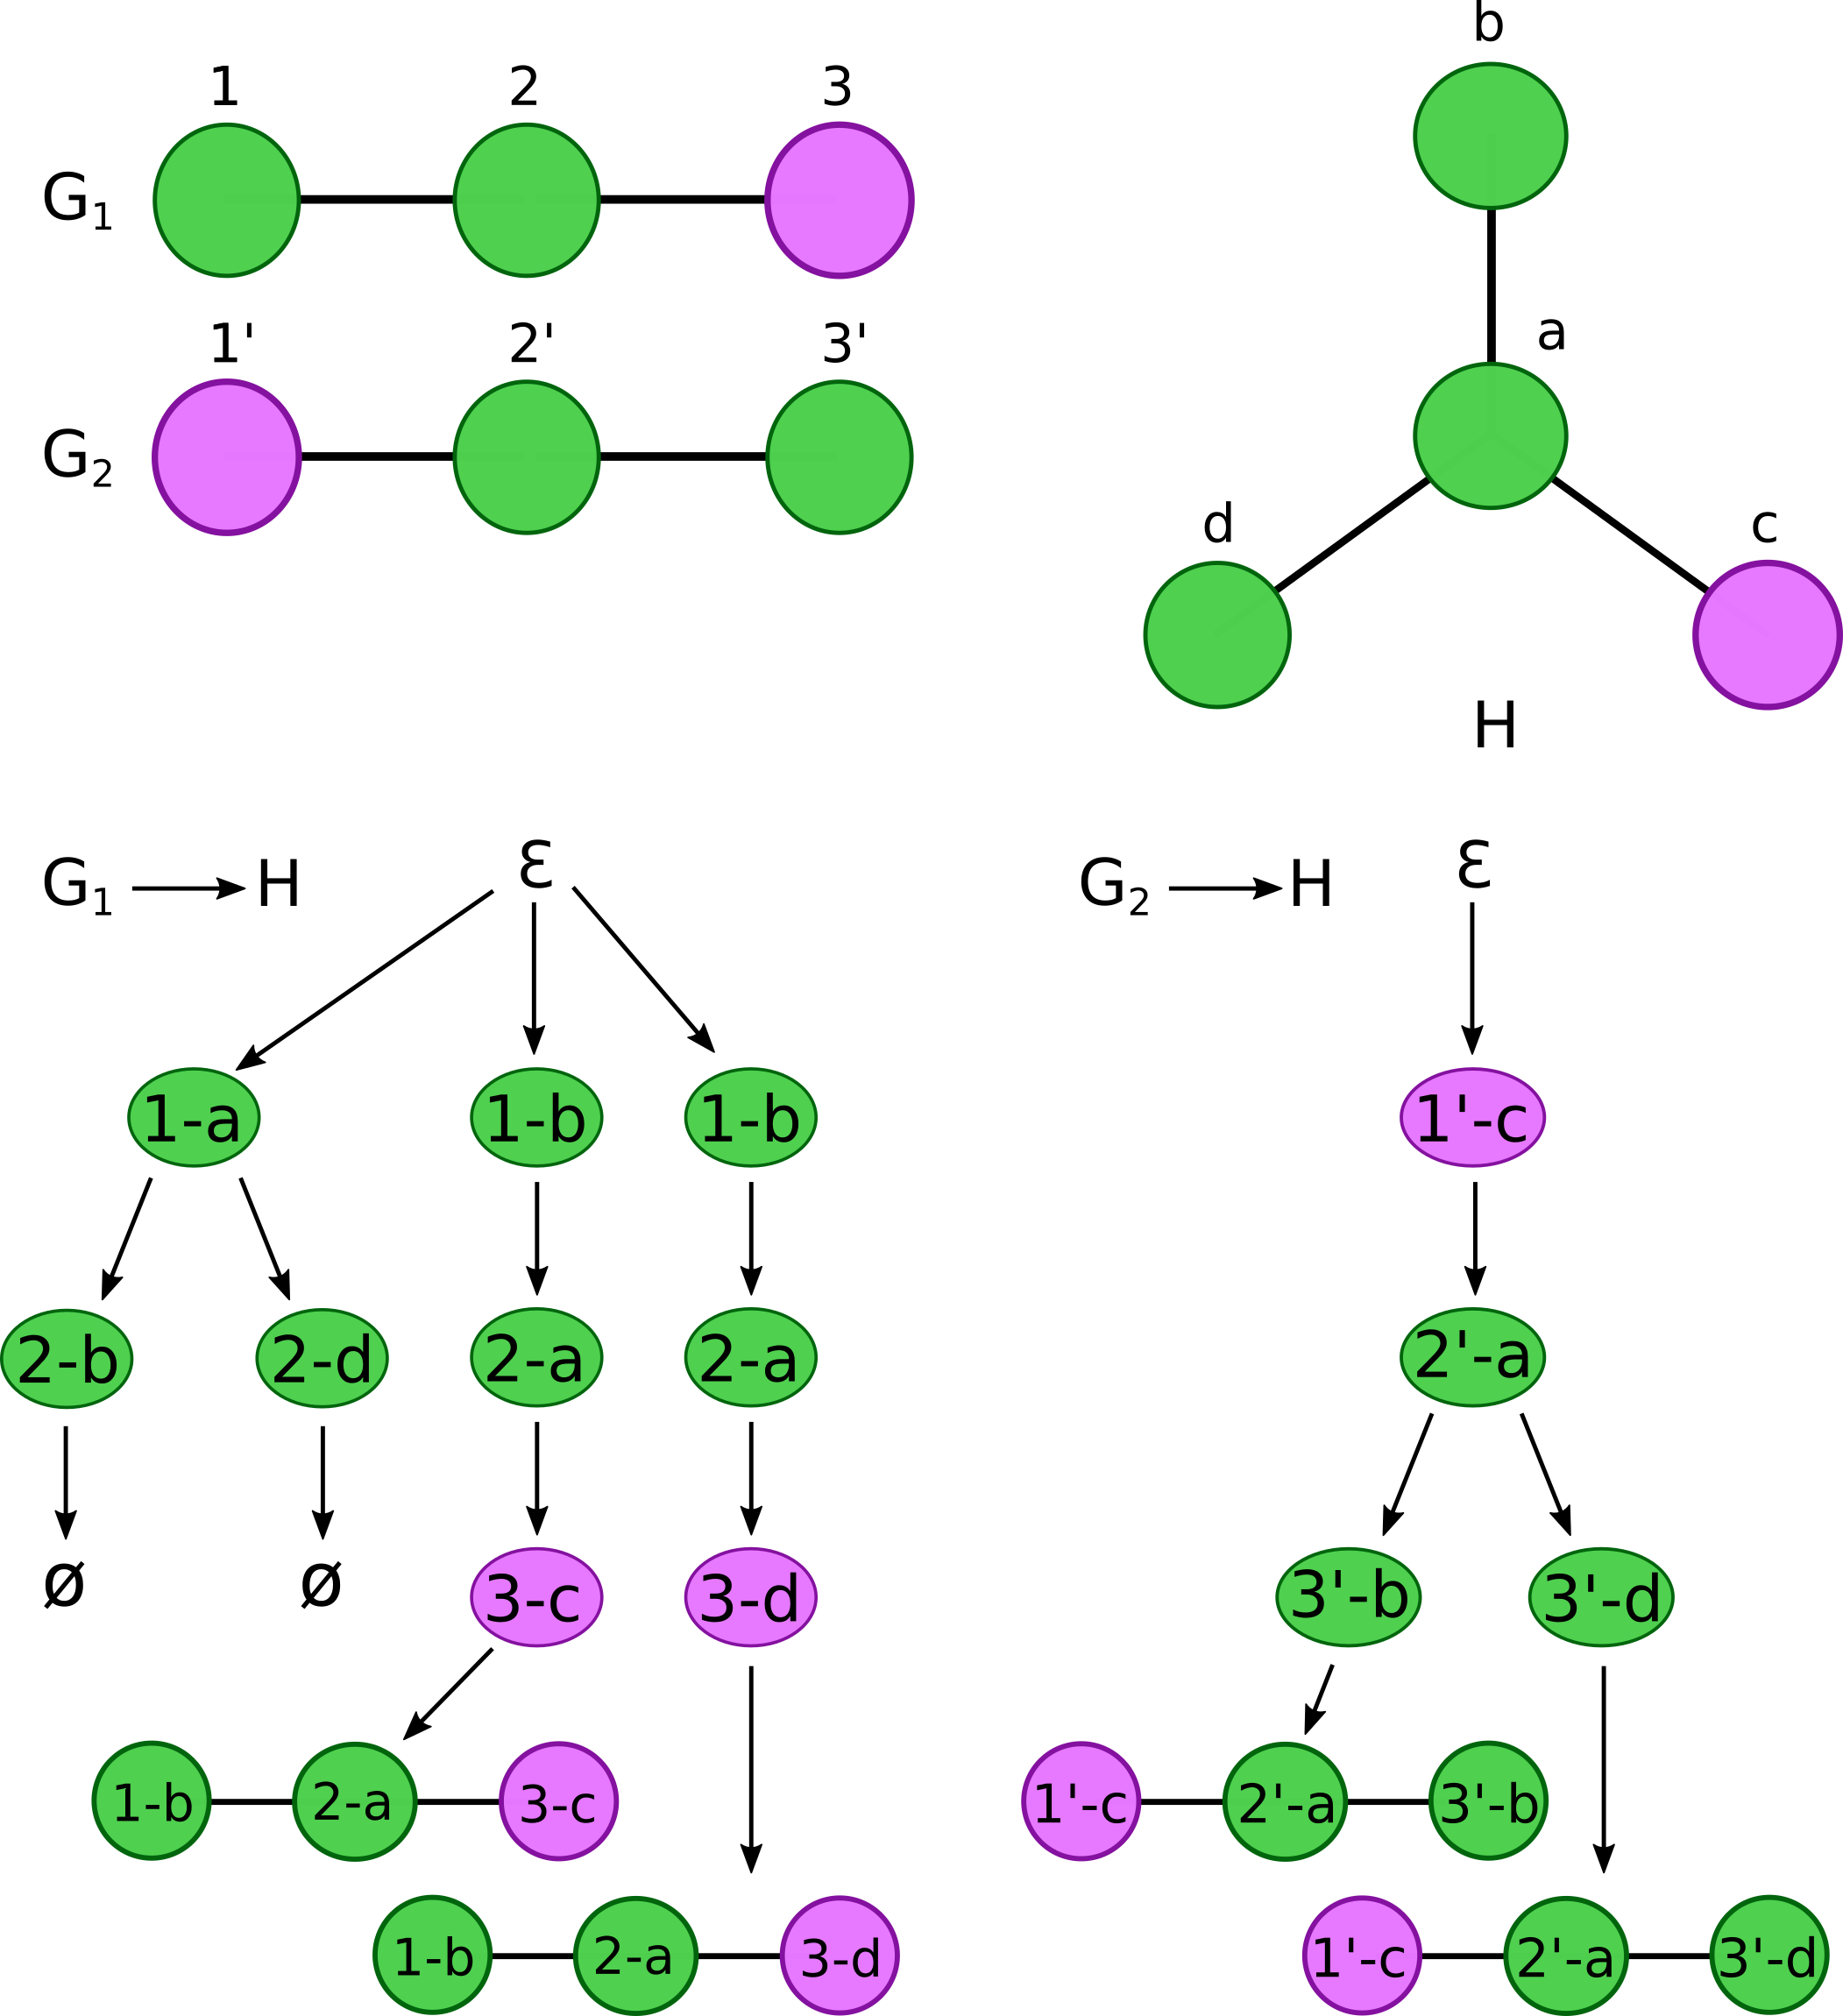
\includegraphics[width=350px]{Figures/s2m/recherche/VF2_labels.png}
    \caption{\label{vf2_labels}Modification de VF2 pour son application aux graphes étiquetés.
    On voit nettement sur cet exemple que l'ordre de recherche des labels influence le temps d'exécution de l'algorithme.}
  \end{center}
\end{figure}

Intéressons nous à l'application de VF2 aux graphes étiquetés.
L'algorithme peut être modifié pour ne former que des paires de n\oe{}uds de même étiquette.
Prenons à nouveau notre exemple précédent en étiquetant avec A et B les n\oe{}uds.
Sur la figure \ref{vf2_labels}, on peut voir la recherche d'un graphe $G$ composé de 2 n\oe{}uds A et un n\oe{}ud B au sein d'un graphe $H$
composé d'un branchement supplémentaire contenant un n\oe{}ud B.
Sur ce graphique nous avons représenté deux cas de recherche selon l'ordre dans lequel nous prenons $G$.
Nous pouvons remarquer que, dans les deux cas, la taille de l'arbre est bien plus faible que pour un graphe non étiqueté.
Les étiquettes des n\oe{}uds font office de filtres de recherche et accélèrent fortement la recherche.
On voit également que la recherche est d'autant plus rapide que l'on choisit prioritairement les n\oe{}uds avec des étiquettes de faible fréquence.

Là où l'algorithme général VF2 était en $O(n^m)$, la complexité est ici réduite dans le pire des cas à $O(k^n)$ où $k$ est le comptage du nombre de n\oe{}uds de l'étiquette la moins filtrante.
La taille de l'arbre de recherche est diminuée par la sélectivité des étiquettes de n\oe{}uds.
Pour optimiser la recherche, nous devons donc étudier la façon dont nous représentons les molécules afin d'avoir une sélectivité
la plus grande possible.

\subsubsection{Sélectivité d'un n\oe{}ud}

\label{selectiv_p}

Premièrement, attachons nous à la représentation la plus basique possible d'un graphe chimique (atome=n\oe{}ud, liaison=arête).
Dans cette représentation, nous pouvons considérer chaque étiquette comme étant le nom de l'atome du n\oe{}ud (Voir figure \ref{representations}, première partie).
Bien entendu, les hydrogènes sont les atomes les plus représentés et ne filtrent pas les recherches par eux-mêmes.
Cependant, ils contiennent une information supplémentaire sur l'atome auquel ils sont liés.
Ainsi, trouver un $CH_{3}$ ou un $CH$ donne une information différente sur la topologie.
En prenant en compte la remarque précédente, nous avons créé une seconde représentation qui compresse les hydrogènes à l'intérieur des n\oe{}uds représentant les atomes plus lourds.
Ainsi, plusieurs étiquettes différentes peuvent désormais être créés pour un même atome et ce, en fonction de ses compagnons hydrogènes (Voir figure \ref{representations}, seconde partie).
Par exemple $NH_2$, $NH$, $N$ sont les trois étiquettes variants depuis l'ancienne étiquette unique $N$ qui était accompagnée de voisins hydrogènes.
Les étiquettes sont plus nombreuses et leur fréquence à la fois moins élevée et plus homogène, ce qui les rend plus sélectives.

\begin{figure}[!ht]
  \includegraphics[width=300px]{Figures/s2m/representations/all_tmp.pdf}
  \caption{\label{representations}Manque fréquences et titres dans l'image}
\end{figure}

Globalement, au plus le nombre d'étiquettes est élevé et au plus les fréquences de ces étiquettes sont homogènes, au moins l'algorithme VF2 aura de difficultés à effectuer un isomorphisme.
En effet, la lenteur qui peut venir de cet algorithme est due aux nombreux chemins qu'il
peut prendre lors de l'exploration.

Cherchons encore à augmenter la sélectivité des étiquettes en augmentant leur nombre.
A partir d'un graphe $G$, il est possible de représenter ses relations d'adjacence au sein d'un second graphe nommé $L$.
Pour cela, deux n\oe{}uds voisins de $G$ sont représentés dans $L$ comme un seul n\oe{}ud (voir line-graph2 dans figure \ref{representations}).
Chaque ancienne arrête devient un n\oe{}ud et chaque ancien n\oe{}ud devient une multitude d'arêtes (une clique entre tous les nouveaux n\oe{}uds représentant les anciennes arêtes de cet ancien n\oe{}ud).
Nous étendons le raisonnement pour les étiquettes en disant que l'étiquette d'un n\oe{}ud du nouveau graphe est la composition des étiquettes des anciens n\oe{}uds ainsi que de l'arité entre ces deux n\oe{}uds.
Dans notre cas, les étiquettes sont mises dans l'ordre lexicographique pour ne pas avoir deux étiquettes possibles à partir des étiquettes d'origine.
Un tel type de graphe est appelé \textit{line graph}~\cite{orlin_line-digraphs_1978}.
L'inclusion de l'arité du lien dans les étiquettes est un très gros avantage de cette représentation.
La fonction de recherche n'aura donc plus du tout à s'attarder sur le degré des arêtes.
De plus, transformer les graphes de cette manière nous permet de répondre à la volonté d'augmenter le nombre d'étiquettes.
Là où la représentation précédente pouvait avoir $n$ étiquettes différentes, celle-ci pourra générer plus de $n^2$ ($3n^2$ si on compte tous le degré des liaisons entre atomes).

Le raisonnement des line graphe peut être étendu récursivement.
On peut ainsi créer des \textit{line-graph} de \textit{line-graph}.
Cependant, dans notre cas, cela pose plusieurs problèmes de répéter cette opération.
La répétition de l'opération de transformation diminuera la taille de certains graphes jusqu'à ce qu'ils disparaissent totalement.
Dans d'autres graphes, le nombre de n\oe{}uds va grandir avec la répétition et ainsi augmenter le nombre de comparaisons nécessaires à la résolution d'un SI.
Pour ces raisons, nous avons choisi de n'effectuer qu'une seule étape de line-graph.

\begin{figure}[!ht]
  \begin{center}
    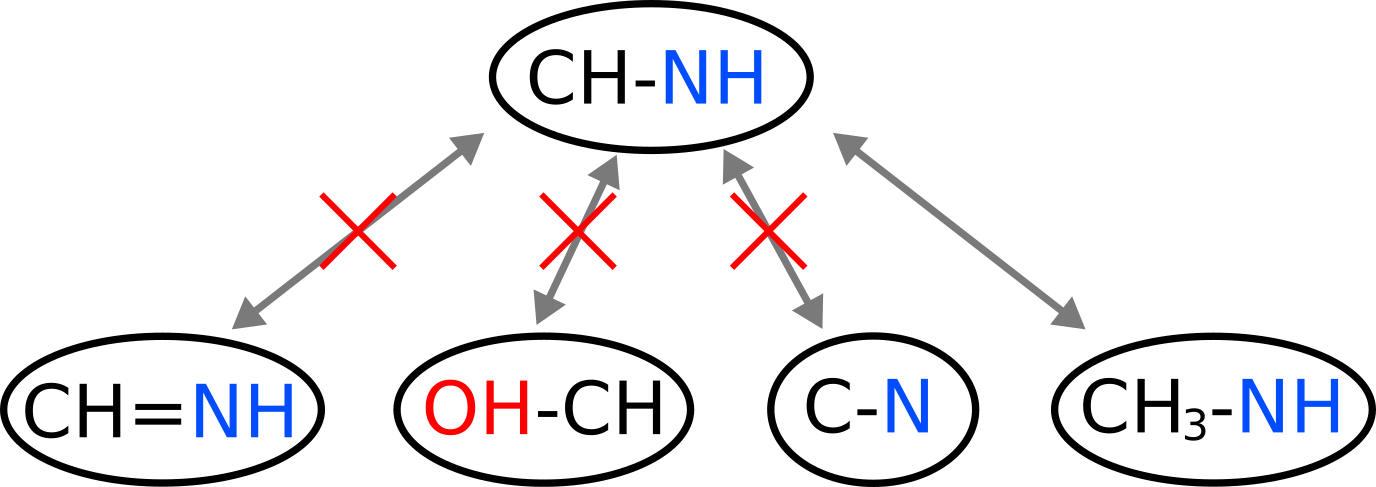
\includegraphics[width=200px]{Figures/s2m/recherche/strict.png}
    \caption{\label{label_matching}Exemple de fonctionnement de la fonction de matching d'étiquettes.
    Le premier n\oe{}ud ne correspond pas au n\oe{}ud car l'arité du lien contenue dans l'étiquette est différente.
    Le deuxième ne correspond pas car les atomes des étiquettes ne correspondent pas.
    Le troisième ne correspond pas car l'étiquette ne contient pas suffisamment d'hydrogènes liés aux atomes principaux.
    Enfin, le dernier remplit les 3 critères précédemment cités et la correspondance est possible.}
  \end{center}
\end{figure}

\subsubsection{Indexation des monomères}

\label{index_p}

Connaissant la sélectivité pour une étiquette, nous cherchons désormais à savoir l'ordre dans lequel il faut rechercher un motif afin de minimiser le temps de recherche.
Nous appellerons \textbf{motif} le graphe compressé que nous allons vouloir retrouver dans un plus
grand graphe. Définissons également une \textbf{chaîne} comme étant un motif plus un \textbf{ordre} dans lequel parcourir ce motif.
Ainsi, on peut avoir plusieurs chaînes représentant le même motif mais avec des ordres de parcours différents.
Ce que nous appellerons \textbf{indexation} sera donc la phase de création d'une chaîne pour représenter chaque motif d'intérêt en essayant de minimiser le temps que prendra la recherche de cette chaîne.
Pour la recherche de monomères dans des peptides non ribosomiques, la phase d'indexation revient donc à choisir, pour chaque monomère, l'ordre dans lequel nous allons rechercher les n\oe{}uds du graphe le représentant.
Ainsi, on peut voir que quelque soit la chaîne représentant le graphe, le même motif sera toujours recherché.
La seule différence sera la rapidité d'exécution de la recherche.
Les deux sections suivantes s'attarderont à la recherche de chaînes performantes (\textit{ie} les plus rapide) lors la recherche d'un motif.


\subsubsection{Indexation gloutonne}

\begin{figure}[!ht]
  \begin{center}
    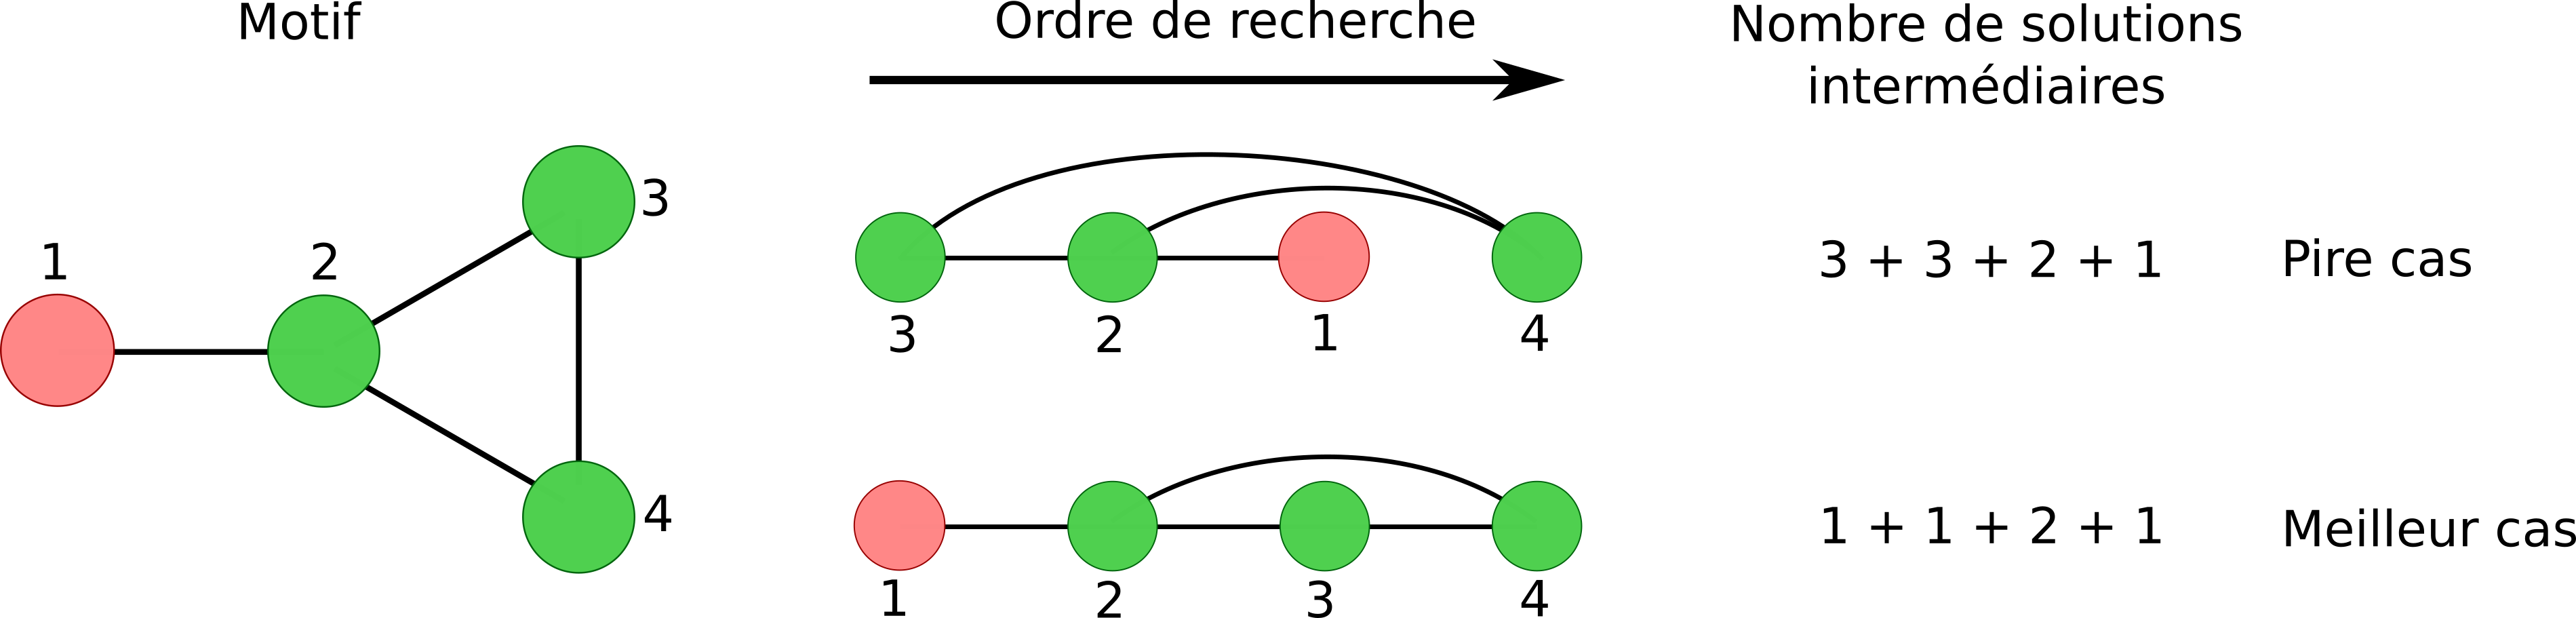
\includegraphics[width=450px]{Figures/s2m/indexation/chaines_example.png}
    \caption{\label{chaine_fail}Deux exemple de chaîne pour un motif simple}
  \end{center}
\end{figure}

Une chaîne efficace est donc une chaîne rapide.
Déterminons quel(s) critère(s) simple(s) nous permettent de supposer qu'une chaîne est efficace.
Avec ce ou ces critères, nous pourrons ensuite déterminer un moyen d'ordonner les n\oe{}uds de manière gloutonne.
Partons de l'exemple présenté sur la figure \ref{chaine_fail}.
A gauche est dessiné un motif simple suivi de deux chaînes pouvant le représenter (lecture de l'ordre des chaînes de gauche à droite).
Pour la première chaîne, en partant du motif ne contenant qu'un A, on obtiendra 3 isomorphismes.
En étendant ces chaînes à deux A voisins, on conserve toujours trois isomorphismes puis deux en ajoutant B et enfin un seul avec le dernier A.
Au total, on aura étendu 9 isomorphismes durant la recherche.
En regardant maintenant la seconde chaîne, on se rend compte que le nombre de ces isomorphismes intermédiaires est bien plus faible grâce à la sélectivité du B recherché en tout premier (5 isomorphismes intermédiaires sont étendus).
La différence décisive entre les deux chaînes est donc le moment où le n\oe{}ud avec une étiquette sélective est recherché.
Effectivement, si le n\oe{}ud B est recherché dès le début, la solution est ``ancrée'' sur une base solide et ne risque a priori pas de créer trop de solutions intermédiaires qui devront toutes être analysées pour passer à l'étape suivante.
On peut dire qu'un n\oe{}ud est plus sélectif qu'un autre à partir du moment où sa fréquence d'apparition dans les molécules étudiées est moins élevée.

\textbf{Étiquettes fréquentes}

\begin{figure}[!ht]
  \begin{center}
    \includegraphics[width=350px]{Figures/s2m/indexation/apprentissage.png}
    \caption{\label{apprentissage}En haut de l'image est représentée la base d'apprentissage puis en bas, le motif qui doit être indexé ainsi que les fréquences d'apparition de chacun de ses n\oe{}uds dans la base d'apprentissage}
  \end{center}
\end{figure}

Essayons d'estimer ces fréquences afin d'éviter les cas qui pourraient être critiques.
Pour ce faire, nous pouvons constituer un ensemble représentatif du type de molécules que nous allons analyser.
Dans notre cas, nous cherchons à étudier des peptides non ribosomiques.
La base d'apprentissage des fréquences sera donc constituée de NRP dont la composition atomique est déjà connue.
Le raisonnement est extensible à n'importe quel type de molécules et le fait d'avoir un jeu d'apprentissage peu ou pas représentatif n'influencera pas le résultat mais uniquement le temps de calcul.
Une fois cette base créée, nous pouvons estimer les fréquences d'apparition de chacune des étiquettes présentes dans les monomères en effectuant une recherche exhaustive (Figure \ref{apprentissage}).

% 
%   \begin{algorithm}[H]
%     \caption{Algorithme glouton de création de l'ordre des n\oe{}uds pour le parcours d'un graphe}
%     \KwData{Un graphe $G(V,E)$}
%     \KwResult{Une liste $N$ contenant tous les n\oe{}uds de V ordonnés pour la recherche}
%     \SetKwFunction{recur}{recur}\SetKwFunction{algo}{trier}
%     \SetKwProg{myalg}{fonction}{}{}
%     \myalg{\algo{$G(V,E)$}}{
%       \KwRet \recur{$G(V,E)$, \{\}}\;
%     }
%  
%     \myalg{\recur{$G(V,E)$, $N$}}{
%       \eIf {$|N| == |V|$}{
% 	\KwRet $N$\;
%       } {
% 	Prendre tous les voisins des n\oe{}uds présents dans $N$ qui ne sont pas présent dans $N$\;
% 	Choisir le n\oe{}uds $n$ avec l'étiquette la moins fréquente\;
% 	Ajouter $n$ à la fin de $N$\;
% 	\KwRet \recur {$G(V,E)$, $N$}\;
%       }
%     }
%   \end{algorithm}


Un algorithme glouton naïf vient tout de suite en tête.
Il est possible de choisir un à un les n\oe{}uds que l'on souhaite ajouter au motif en prennant toujours celui avec l'étiquette la moins fréquente.
Il est nécessaire de préciser que la recherche des n\oe{}uds voisins peut être faite en maintenant un ensemble des voisinages.
L'algorithme glouton naïf est donc linéaire par rapport à la taille du graphe.
À l'exécution, la création de chaînes par cette méthode est instantanée ($\ll$ 0.1s).
Toutefois, rien ne garantit la qualité des chaînes obtenues.
Prenons l'exemple de la figure \ref{apprentissage}.
Sur cet exemple, le motif à indexer est a-b-d.
Les comptages des différentes étiquettes nécessaires sont également présents sur cette même figure.
La chaîne qui sera générée commence forcément par le n\oe{}ud étiqueté $a$ (fréquence la plus faible dans le jeu d'apprentissage) suivi de $b$ puis enfin $d$ (le tout est résumé sur la figure \ref{glouton}).

\begin{figure}[!ht]
  \begin{center}
    \includegraphics[width=400px]{Figures/s2m/indexation/glouton.png}
    \caption{\label{glouton}En vert le chemin pris par l'algorithme glouton pour générer la chaîne du motif a-b-d}
  \end{center}
\end{figure}

\subsubsection{Indexation Markovienne}

\label{index_markov}

En utilisant la méthode gloutonne, nous obtenons rapidement les chaînes de tous les motifs que nous souhaitons indexer.
Cependant, dans certains cas, une chaîne générée de cette manière peut ne pas être optimale.
Dès le tout début de la chaîne, il est possible que l'algorithme fasse des choix localement optimaux qui vont ensuite mener à un enlisement global.
Nous allons nous appuyer sur les figures \ref{apprentissage} et \ref{glouton} pour monter que même sur un si petit exemple, l'algorithme glouton n'a pas choisi le meilleur chemin.

Afin d'évaluer la qualité d'une chaîne, nous allons calculer son temps d'exécution sur notre base d'apprentissage.
Partons de la définition d'une chaîne : une chaîne est composée d'une succession de n\oe{}uds.
Ces n\oe{}uds vont, lors de l'isomorphisme, être recherchés dans l'ordre donné par la chaîne.
Pour rechercher une chaîne de taille $n$ ($c_n$), il faut donc $n$ extensions successives.
On peut donc écrire que le temps de recherche d'une chaîne est le temps cumulé de recherche de ses extensions :

\begin{equation}
 T(c_n) = T(p_0 \rightarrow p_1 \rightarrow ... \rightarrow p_n) = \sum_{i=1}^n T(p_{i-1} \rightarrow cp_i)
\end{equation}

Où $T()$ est la fonction représentant le temps de recherche d'une chaîne, $p_i$ le un motif de taille $i$ et $p_{i-1} \rightarrow p_i$ la dernière extension d'une chaîne $c_i$ représentée par le passage du motif $p_{i-1}$ au motif $p_i$.
Il est à noter que rechercher une chaîne de taille 1 revient à étendre un motif vide.
C'est à dire qu'il est nécessaire de parcourir l'intégralité des n\oe{}uds de la cible dans laquelle on recherche le motif et ce quel que soit le motif.
Sur notre base d'apprentissage il faudra donc toujours tester tous les n\oe{}uds de tous les peptides d'apprentissage pour la première extension.
% 
% \begin{figure}
%   \begin{center}
%     \includegraphics[width=300px]{Figures/s2m/indexation/arite.pdf}
%     \caption{\label{arrite}Arité restante pour les différents n\oe{}uds d'un graphe chimique simple}
%   \end{center}
% \end{figure}

Lors d'une recherche d'une chaîne $c_{n-1}$, il est possible de trouver des isomorphismes sur la cible (potentiellement partiellement recouvrant).
Afin de calculer le temps de recherche de $c_n$ nous devons prendre en compte la quantité de sous-isomorphismes précédemment trouvés.
Le calcul du temps de recherche de $c_n$ correspondra donc au temps de calcul de $c_{n-1}$ auquel on vient ajouter le temps de recherche de la dernière extension sur chacun des isomorphismes de taille $n-1$.
Il faut également tenir compte du nombre d'extensions qui vont être essayées.
Par exemple, si l'on cherche à étendre un isomorphisme précédent en suivant un lien qui est enraciné sur un $NH$, il ne reste qu'une liaison à explorer (le $N$ ayant déjà une liaison avec son $H$ et une liaison avec le reste du motif déjà recherché).
En reprenant la même logique pour un seul carbone, il resterait donc trois autres liaisons à suivre.
Nous appellerons cette quantité l'\textit{arité restante}.
On peut donc écrire :

\begin{equation}
 T(p_{n-1} \rightarrow p_n) = n_{p_{n-1}} \times a_{p_{n-1} \rightarrow p_n} \times t
\end{equation}

où $n_{p_{n-1}}$ est le nombre d'isomorphismes trouvés pour le motif $p_{n-1}$, $a_{p_{n-1} \rightarrow p_n}$ est l'arité restante
de l'atome depuis lequel on étend le motif $p_{n-1}$ vers le motif $p_n$ et $t$ le temps nécessaire pour une comparaison de deux
étiquettes (ce temps peut être considéré constant)

Combinons les deux équations précédentes, pour obtenir une formule globale :

\begin{equation}
 T(c_n) \propto^t N + \sum_{i=2}^n (n_{p_{i-1}} \times a_{p_{i-1} \rightarrow p_i})
\end{equation}

où $N$ est le temps de calcul pour les chaines de taille 1.
Ce temps ne varie par car il est nécessaire de parcourir tout le graphe.

\begin{figure}[!ht]
  \begin{center}
    \includegraphics[width=400px]{Figures/s2m/indexation/apprentissage_comptage.png}
    \caption{\label{app_compt}Base d'apprentissage accompagnée des comptages de tous les $n_{p_{n}}$}
  \end{center}
\end{figure}

En utilisant les comptages faits sur la base d'apprentissage (voir \ref{app_compt}) ainsi que le calcul de l'arité
restante de chaque n\oe{}ud à chaque étape, nous allons pouvoir estimer sur la base, un temps d'exécution de la recherche d'une
chaîne. Ce temps est un coût exact de la recherche sur la base d'apprentissage. En normalisant cette valeur par le nombre de
n\oe{}uds de la base, nous pouvons ainsi obtenir le coût de recherche par n\oe{}ud et ainsi estimer le temps de calcul, quelle que soit la taille de la, ou des, molécule(s) à analyser.

\begin{equation}
 T(c_n) \propto^t 1 + \sum_{i=2}^n ({n_{p_{i-1}} \over N} \times a_{p_{i-1} \rightarrow p_i})
\end{equation}

Redéfinissons la notation ${n_{p_{i-1}} \over N}$ qui correspond à un taux de filtrage d'un motif de taille $i-1$.
Appelons ce taux $F_{i-1}$. Cette notation peut à son tour être transformée en
produit des filtrages de chaque extension d'une chaîne. Les valeurs des filtrages estimés s'obtiennent immédiatement à partir des
comptages dans la base d'apprentissage (Voir l'exemple en figure \ref{app_compt}).
Il est à noter que le taux de filtrage peut être supérieur à 1 dans le cas où la recherche obtient plus d'isomorphismes en cours de création à la suite de l'ajout du n\oe{}ud.

\begin{equation}
 {n_{p_{i-1}} \over N} = F_{i-1} = \prod_{i=0}^{i-1} f_i
\end{equation}

\begin{equation}
 T(c_n) \propto^t 1 + \sum_{i=2}^n a_{p_{i-1} \rightarrow p_i} \prod_{j=0}^{i-1} f_j
\end{equation}

Le temps de recherche optimal d'un motif est donc le temps de recherche de la chaîne qui minimise le coût. Donc :

\begin{equation}
 T(p_n) = \min_{\forall c_n} T(c_n)
\end{equation}


Appliquons maintenant cette formule de calcul du temps sur notre exemple pour trouver la meilleure chaîne possible par
rapport à la base d'apprentissage. Pour le motif de l'exemple de la figure \ref{app_compt}, nous pouvons nommer les différentes chaînes possibles de $\alpha$
jusque $\delta$.

\[
\begin{array}{ccccccc}
 c         & = & p_1 & \rightarrow & p_2     & \rightarrow & p_3 \\
 c_\alpha  & = & a   & \rightarrow & a\!-\!b & \rightarrow & a\!-\!b\!-\!d \\
 c_\beta   & = & b   & \rightarrow & a\!-\!b & \rightarrow & a\!-\!b\!-\!d \\
 c_\gamma  & = & b   & \rightarrow & b\!-\!d & \rightarrow & a\!-\!b\!-\!d \\
 c_\delta  & = & d   & \rightarrow & b\!-\!d & \rightarrow & a\!-\!b\!-\!d \\
\end{array}
\]

On peut appliquer la formule sur chacune des chaînes possibles et trouver la chaîne optimale qui minimise la fonction de
coût. Développons l'exemple pour la chaîne $c_{\alpha}$.

\[
\arraycolsep=1.4pt\def\arraystretch{1.2}
\begin{array}{cccccccccccccc}
  c_\alpha    & =  & \epsilon &  \rightarrow &  \multicolumn{3}{c}{a} & \rightarrow & \multicolumn{3}{c}{a\!-\!b} &  \rightarrow & \multicolumn{1}{c}{a\!-\!b\!-\!d} &\\
  T(c_\alpha)   & =  & T( \epsilon &  \rightarrow &  a)  & + & T( a &  \rightarrow  & a\!-\!b) & + & T(a\!-\!b &  \rightarrow & a\!-\!b\!-\!d) &\\
                    & \propto_{N}  &  \multicolumn{3}{c}{1} &  + & \multicolumn{3}{c}{3 \times \frac{2}{18}} & + & \multicolumn{3}{c}{  (3-1)\times \frac{2}{18} \times \frac{3}{2}} &\\
                    & = &  \multicolumn{3}{c}{1} &  + & \multicolumn{3}{c}{\frac{1}{3}} & + & \multicolumn{3}{c}{\frac{1}{3}}   & \quad= \quad\frac{5}{3} \\

\end{array}
\]

En appliquant cette formule sur toutes les chaînes, on peut se rendre compte que certains de nos calculs sont inutiles.
Prenons l'exemple des chaînes $c_{\alpha}$ et $c_{\beta}$. Le dernier calcul de la chaîne $c_{\beta}$ est inutile. Lors
du calcul des deux chaînes, on aurait pu se rendre compte que l'on pouvait déjà décider de quelle chaîne était la meilleure à
partir du résultat de la sous chaîne $a-b$. Ceci nous amène à transformer le calcul sous forme de programmation dynamique dont les
formules de récurrence sont les suivantes.


\begin{equation}
 T(\epsilon \rightarrow p_1) = 1
\end{equation}
\begin{equation}
 T(p_n) = \min_{\forall p'_{n-1} \subset p_n} (T(p'_{n-1}) + T(p'_{n-1} \rightarrow p_n))
\end{equation}

où la fonction de minimisation s'applique sur l'ensemble des $p'_{n-1}$ et $p'_{n-1}$ est un motif connexe de taille $n-1$ inclus
dans $p_n$. Pour la recherche de motif dans l'exemple, on obtient le chemin $c_{\delta}$ minimisant le coût. On peut voir le
détail de la recherche de ce motif sur la figure \ref{markov}.

\begin{figure}[!ht]
  \begin{center}
    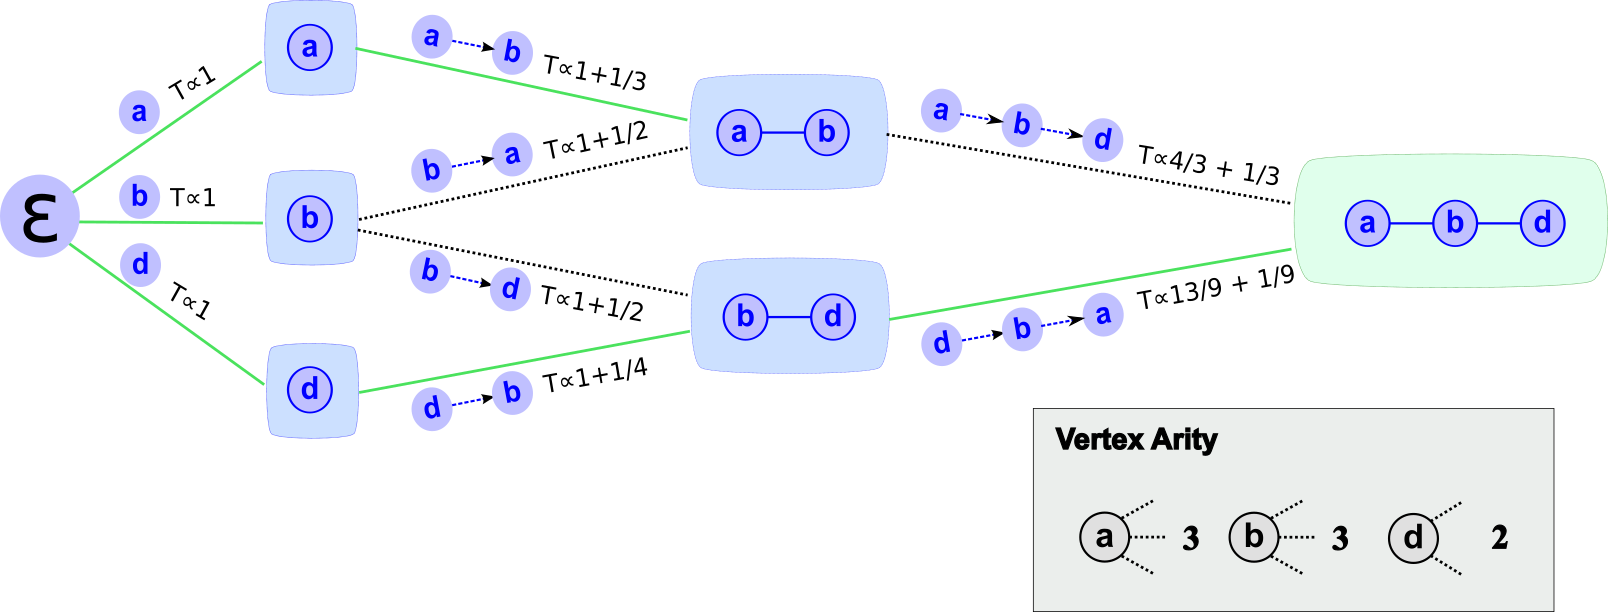
\includegraphics[width=400px]{Figures/s2m/indexation/markov.png}
    \caption{\label{markov}En vert, le chemin optimal pris par l'algorithme markovien pour générer la chaîne du motif a-b-d}
  \end{center}
\end{figure}

Cette méthode exacte nous permet de garantir la qualité de nos chaînes sur la base d'apprentissage mais cela se paye logiquement en temps de pré-calcul.
En effet, même par programmation dynamique le temps de pré-calcul des chaînes est très élevé si les motifs sont composés de nombreux branchements et d'une grande diversité de n\oe{}uds.
Calculons la complexité, en considérant que chaque étiquette est unique, sur les deux cas extrêmes~: une ligne et une clique.

Une ligne représente le motif le plus simple.
Pour une ligne de n\oe{}uds de taille $n$, on peut trouver un motif de taille $n$ puis deux de taille $n-1$ puis 3 de taille $n-2$, ...
Pour calculer le coût du motif de taille $n$, il nous faut calculer récursivement tous les motifs de taille inférieure.
Dans le meilleur des cas la programmation dynamique sera donc de complexité de l'ordre de $n^2$.

Le pire motif (théorique en non chimique) qui peut être défini est une clique.
Dans le cas d'une clique de taille $n$, pour calculer le coût du motif, il faudra calculer $n-1$ parmi $n$ valeurs puis $n-2$ parmi $n$, ... Dans ce cas, la complexité sera de l'ordre de $2^n$.

La redondance des étiquettes permet quant à elle de couper certaines branches lors de l'indexation et ainsi de diminuer un peu la complexité en pratique.
Cependant, l'ordre de grandeur n'en est pas modifié.

\begin{equation}
 Cplx_{chaine} = n + n-1 + ... + 2 + 1 = \sum_{i=1}^n i = {{n (n+1)} \over 2} = O(n^2)
\end{equation}
\begin{equation}
 Cplx_{clique} = {n \choose n} + {n \choose n-1} + ... + {n \choose 2} + {n \choose 1} = \sum_{k=1}^n {n \choose k} = O(2^n)
\end{equation}


\subsubsection{Indexation hybride}

Dans un exemple de la figure \ref{markov}, nous avons montré que le début d'une chaîne est très critique lors de sa recherche dans un graphe.
L'idée est donc de générer la chaîne par un mélange des deux techniques précédentes.
Les débuts de la chaîne seront recherchés en exact jusqu'à une taille $k$ (définie par l'utilisateur à l'avance), puis le reste des extensions se feront en utilisant l'algorithme glouton.
Cette découpe des chaînes en deux parties garantit une recherche très rapide d'un motif sur la base d'apprentissage tout en limitant fortement le temps de pré-calcul nécessaire pour la construction de l'index.



\subsection{Des monomères aux résidus}
\label{families}


\subsubsection{Résidus}

L'algorithme et les indexes présentés dans la section précédente permettent de retrouver rapidement toutes les occurrences d'un motif au sein d'une molécule cible.
Jusqu'à présent nous avons pris l'hypothèse que nous recherchions des monomères dans des peptides.
Ceci n'est en fait pas applicable directement.
En effet, on ne retrouve jamais un monomère en entier au sein d'un polymère.
Lorsque les monomères sont liés entre eux pour former le polymère, chacun perd une partie de ses atomes dans ces liaisons.
Nous appellerons les molécules incluses (monomères sans atomes de liaison) des \textbf{résidus}.

Prenons l'exemple de la Cystéine pour bien comprendre (Voir figure \ref{cys_ex}).
La cystéine est présente dans 47 peptides de la base de données NORINE.
Dans certains peptides comme ACV, la cystéine est incluse en effectuant deux liaisons peptidiques avec ses voisins.
D'un côté, elle perd les atomes $OH$ de son groupement $COOH$ pour aller se lier à un groupe $NH_2$ qui perd un de ses $H$. 
Le tout libère un $H_2O$ pendant la réaction.
De l'autre côté, elle perd un $H$ de son groupement $NH_2$ pour effectuer la même opération inversée.
Au total, la cystéine présente dans ce peptide a donc perdu trois atomes sur deux sites distincts.
Dans d'autre peptides comme dans la malformin A1, la cystéine effectue une troisième liaison au niveau de son atome de soufre en perdant un atome d'hydrogène pour se lier avec un autre atome de soufre et ainsi réaliser un pont disulfure.
Sur ce simple exemple, on remarque que non seulement le monomère n'est jamais inclus en entier mais en plus, il peut être inclus dans un polymère de différentes manières.
Il est donc nécessaire de connaître les différents résidus possibles pour chaque monomère afin de pouvoir les rechercher en utilisant l'algorithme de recherche exact décrit précédemment.

\begin{figure}[!ht]
  \begin{center}
    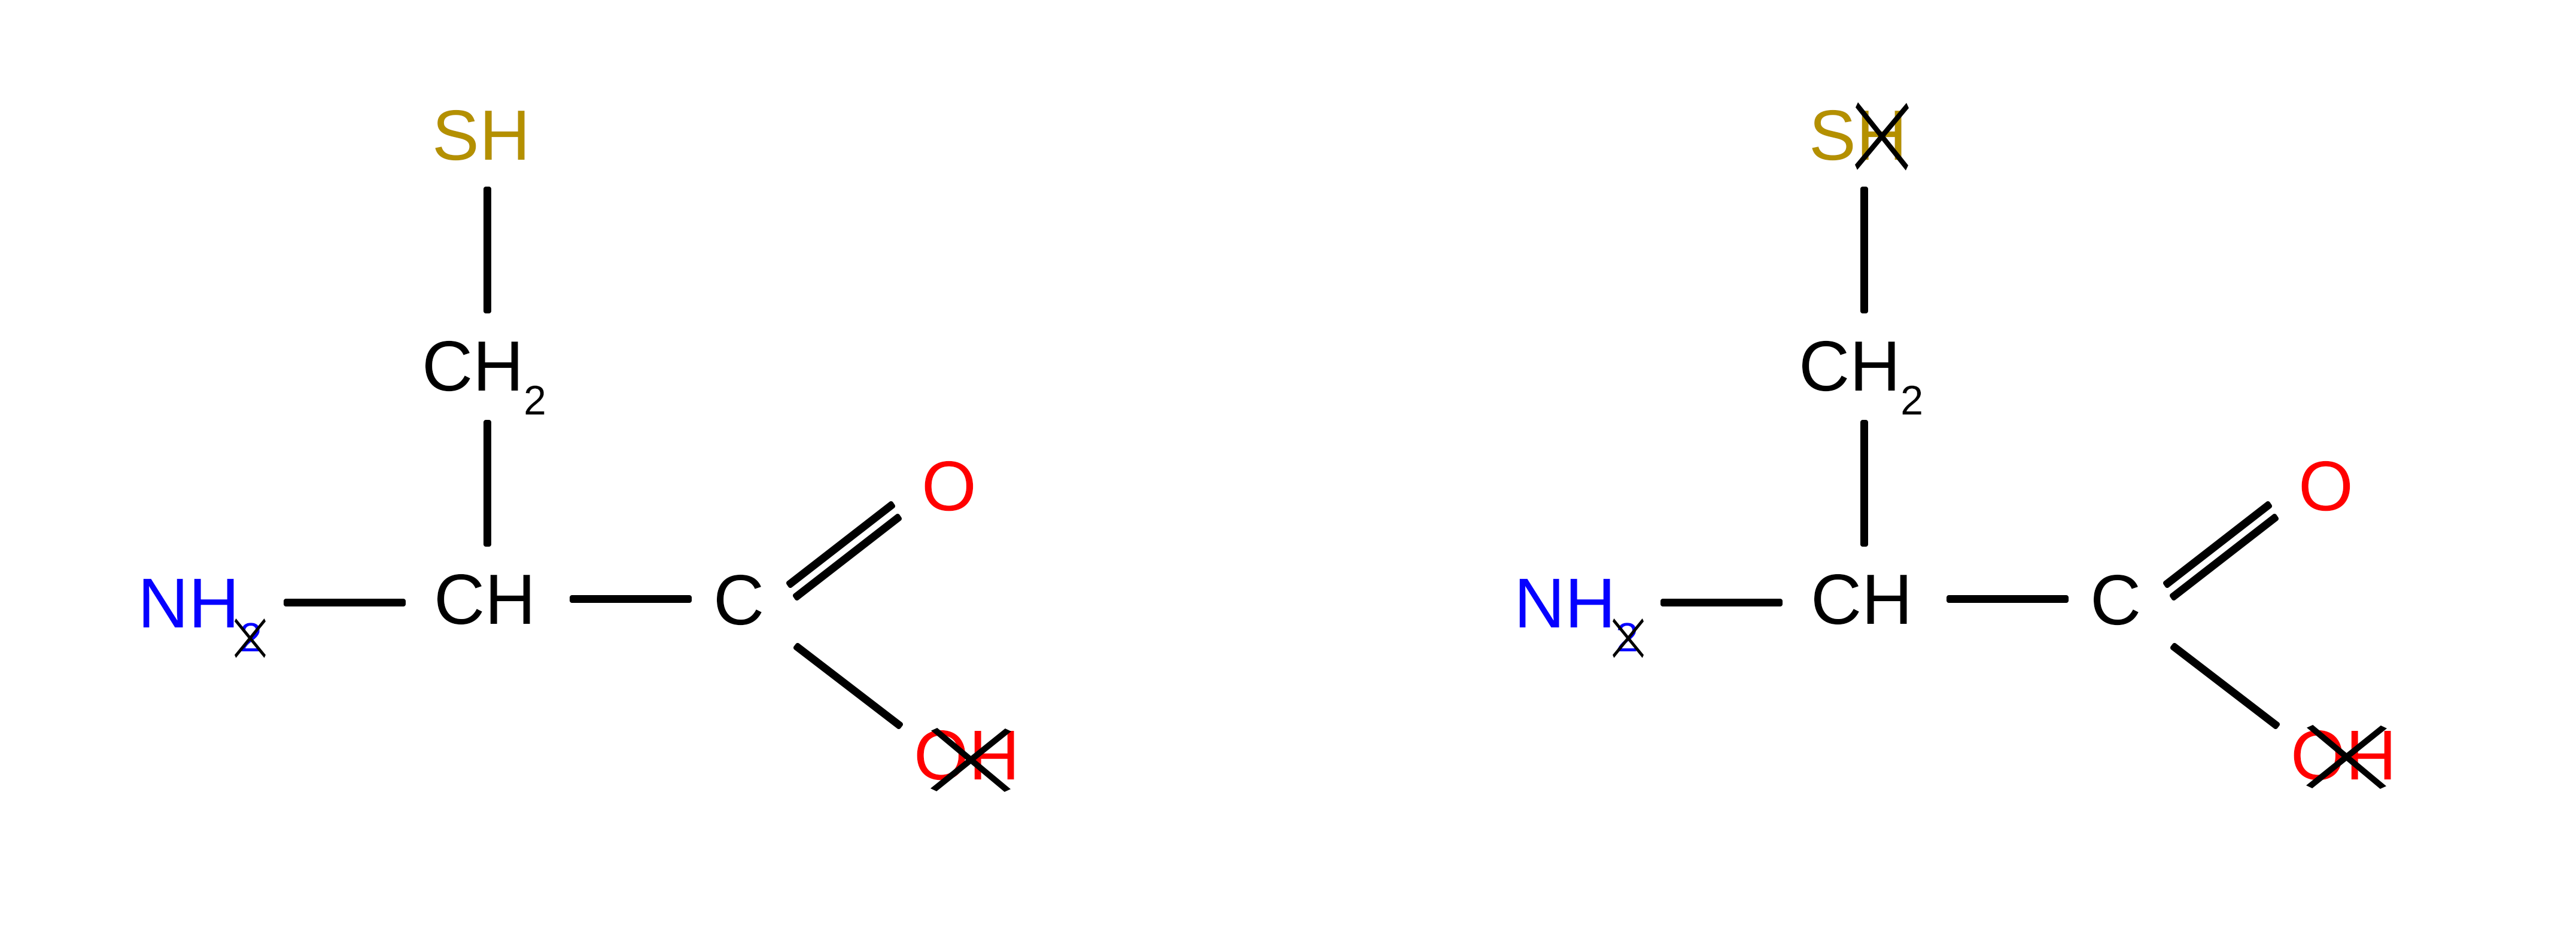
\includegraphics[width=400px]{Figures/s2m/residues/cys_exemple.png}
    \caption{\label{cys_ex}Deux résidus différents présents dans deux peptides différents tout deux obtenus à partir de la Cystéine}
  \end{center}
\end{figure}


\subsubsection{Familles de résidus}

Différents résidus d'un même monomère peuvent être créés selon les contextes.
Pour connaître les différents résidus possibles pour chaque monomère nous devons connaître les règles qui régissent les liaisons.
Par exemple, pour la liaison peptidique précédemment citée, nous pouvons déduire deux règles.
Si un $COOH$ est détecté alors le monomère peut potentiellement perdre son $OH$.
De la même manière, pour la seconde moitié de la liaison, le monomère peut perdre un $H$ pour un $NH_2$ détecté.
En regardant précisément les liaisons qui apparaissent pour un type de polymère, nous pouvons créer une liste de règles de perte d'atomes.
En appliquant ces règles récursivement sur un monomère, nous pouvons générer tous ses résidus candidats.
Notons que certaines règles comme celles du pont disulfure décrite précédemment, ne s'appliquent qu'en présence d'une autre liaison.
Il n'est donc a priori pas nécessaire de générer le résidu qui contient uniquement cette liaison.
Ici nous n'aurons normalement pas de résidus uniquement constituée d'une liaison sulfure.
Il est à noter que, moins une règle sera précise, plus le nombre de résidus générés sera important.
Imaginons une règle qui nous dirait dans un cadre de chimie organique, que ``pour tout carbone lié à au moins un hydrogène, l'atome d'hydrogène peut être perdu pour former une liaison''.
Si $n$ est le nombre d'atomes de carbone dans la molécule ($n$ représente une grande proportion d'atomes dans une molécule organique), alors on peut générer un nombre de résidus de l'ordre de $n^2$.

\begin{figure}[!ht]
  \begin{center}
    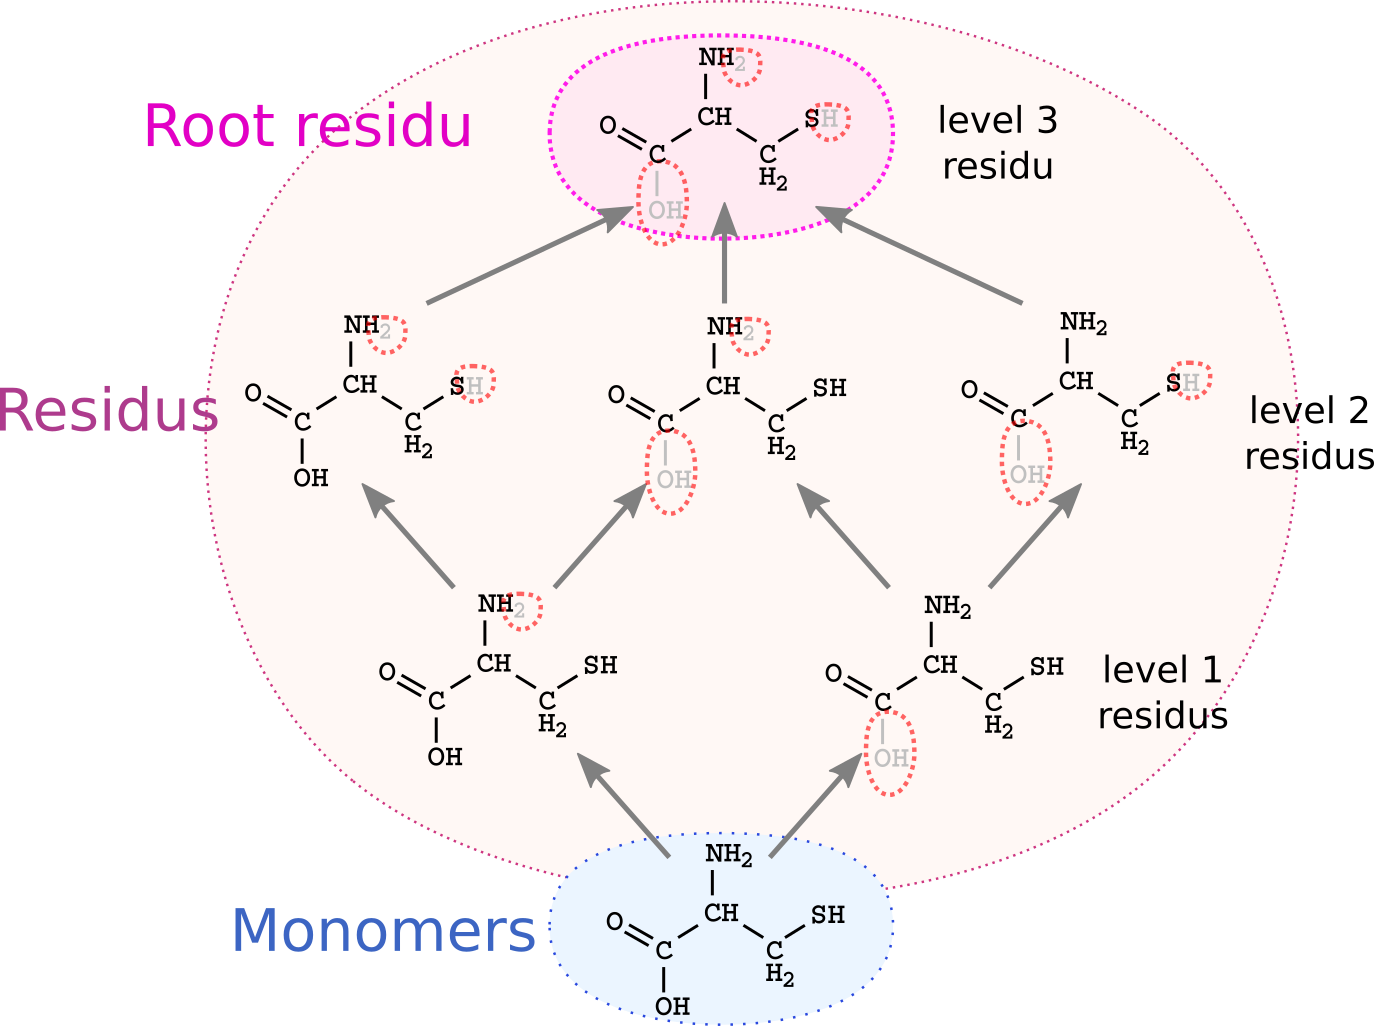
\includegraphics[width=400px]{Figures/s2m/residues/cystein_family.png}
    \caption{\label{family}Représentation de la construction de la famille des résidus de la cystéine.}
  \end{center}
\end{figure}

Comme présenté dans la figure \ref{family}, les différents résidus générés peuvent être représentés sous la forme d'un Graphe Orienté Acyclique (GOA).
Le monomère de base (en bas sur la figure) ainsi que chacun des résidus est un n\oe{}ud du graphe et chaque arc est un lien de parenté entre n\oe{}uds.
Un arc sera par exemple créé entre un résidu auquel on a appliqué une seule règle et le monomère.
Nous appellerons \textbf{famille} cette représentation des résidus sous forme de GOA.

Le n\oe{}ud le plus éloigné du monomère (en haut sur la figure) sera le n\oe{}ud qui aura subi le plus de modifications.
Nous appellerons le résidu de ce n\oe{}ud le \textbf{résidu racine}.
Ce résidu à un intérêt tout particulier pour la recherche du monomère.
En effet, si le résidu racine n'est pas trouvé alors qu'il est celui qui possède le moins d'atomes dans la famille, cela signifie qu'aucun membre de la famille ne pourra être trouvé.
On peut même aller plus loin en étendant le raisonnement à tous les résidus.
Si un résidu de niveau $n$ n'est pas trouvé, alors il est inutile de rechercher ses résidus parents de niveau $n-1$.
Il faut également remarquer qu'il est inutile de chercher un résidu parent de niveau $n-1$ si tout ses enfants de niveau $n$ n'ont pas été trouvés.

En connaissant la structure familiale des résidus ainsi qu'un ordre naturel de recherche pour passer d'un résidu à l'autre, nous pouvons déduire une structure globale de recherche.
Découle donc de cette structure de famille de résidus, un ordre de recherche naturel depuis le résidu racine jusqu'aux résidus de niveau 1 (inutile de rechercher le monomère car il n'étant jamais inclus tel quel).
De plus, il n'est jamais nécessaire de recalculer complètement un isomorphisme une fois que la racine trouvée.
Pour passer d'un résidu $r$ à l'un de ses parents $p$ il suffit de rechercher à étendre l'isomorphisme de $r$ avec les atomes que nous avions considérés perdus pour passer de $p$ à $r$ lors de la construction de la famille.
De plus, le fait de ne pas tout recalculer à chaque étape nous autorise à ne calculer l'index que pour les résidus racine.
Le reste des résidus n'est indexé que sur les extensions à effectuer depuis leurs fils.

% 
% \begin{algorithm}[H]
%   \caption{Algorithme de recherche des résidus d'une famille}
%   \KwData{Un graphe $G(V, E)$ représentant le polymère cible et une famille $F_m$ de résidus pour le monomère $m$. Le résidu $r_r$
%   étant le résidu racine de la famille.}
%   \KwResult{Un ensemble de tuples constitués d'un résidu et d'un ensemble de position. Ces tuples représentent chacun un
%   isomorphisme du résidu avec une sous partie du polymère.}
%   Soit $S$ un ensemble de tuples solution initialement vide\;
%   $S \gets subgraphIsomorphism (G, r_r)$\;
%   
%   \If {$S$ est vide} {
%     \KwRet $S$\;
%   }
%   
%   Soit $P$ un ensemble de résidus à procésser initialisé avec les parents de $r_r$\;
%   \While {$P$ n'est pas vide} {
%     $r \gets supprimeUnElement(P)$\;
%     $Tmp \gets subgraphIsomorphism (G, r)$\;
%     
%     \If {$Tmp$ n'est pas vide} {
%       Ajouter $Tmp$ dans $S$\;
%       \For{$p \subset parents(r)$}{
% 	\If {Tous les enfants de $p$ ont été trouvés} {
% 	  Ajouter $p$ dans $P$\;
% 	}
%       }
%     }
%   }
%   
%   \KwRet $S$;
% \end{algorithm}

\textbf{TODO : figure famille + recherche}

L'algorithme de recherche des résidus ressemble fortement à un algorithme de recherche en largeur.
Nous commençons par rechercher la racine.
Ci celle-ci est trouvée, alors tout ses résidus fils sont recherchés.
Sur l'exemple TODO, le résidu racine de la cystéine est trouvé ; les trois résidus de niveau 2 sont alors recherchés.
Récursivement, lorsqu'un résidu est trouvé, tous ses fils sont recherchés.
Ainsi, la recherche de la cystéine dans le peptide de l'exemple aboutie sur la découverte de 3 isomorphismes de monomères différents.
Ces isomorphismes sont tous situés au même endroit et c'est la phase de pavage qui choisira lequel garder.


\subsection{Pavage de monomères}
\label{pavage_}

\subsubsection{Pavage : définition}

La méthode de recherche des isomorphismes de sous-graphe présentée en section \ref{SI_p}, trouve toutes les occurrences de chacun des monomères dans un peptide cible.

Puisque nous connaissons les atomes contenus dans chacun des isomorphismes découverts, nous pouvons également connaître chacun des isomorphismes découverts par atome.
L'étape de pavage consiste à choisir un sous ensemble des isomorphismes trouvés, de manière à maximiser le nombre d'atomes couverts par un sous ensemble de tout ces isomorphismes, en ayant pour chaque atome, au plus un seul isomorphisme présent dans ce sous ensemble.

\begin{figure}[!ht]
  \begin{center}
    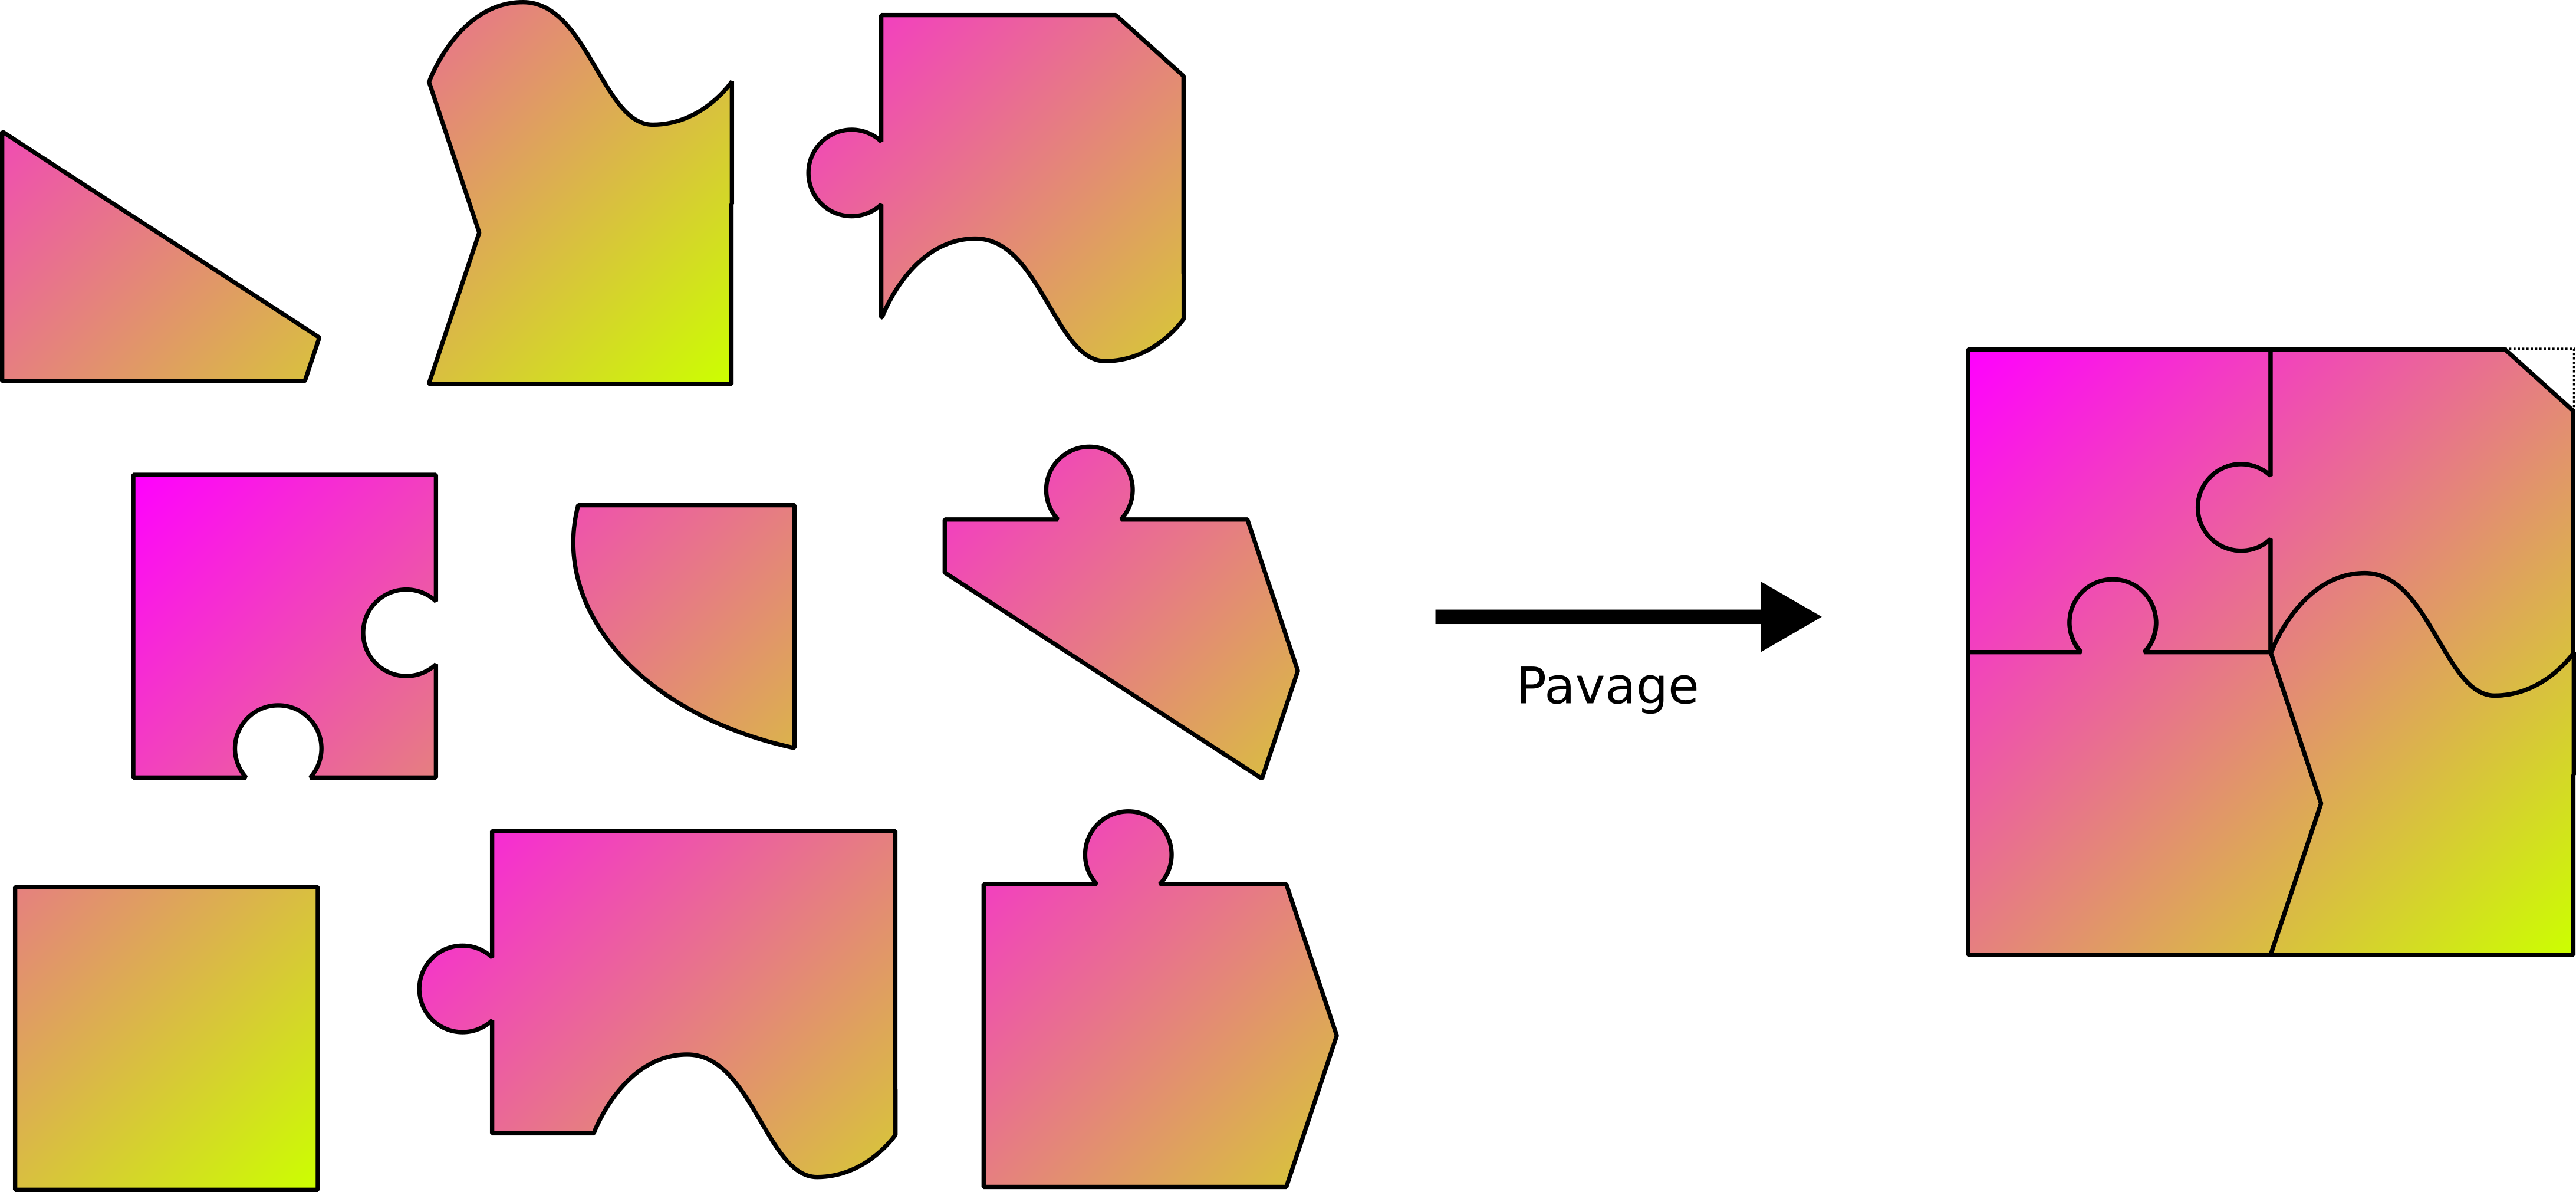
\includegraphics[width=300px]{Figures/s2m/pavage/puzzle.png}
    \caption{\label{puzzle}Phase de pavage.
    Choix parmi toutes les pièces disponibles pour former le puzzle le plus grand possible}
  \end{center}
\end{figure}

Faisons une analogie avec un puzzle. La phase d'isomorphisme créée de nombreuses pièces de puzzle.
Une reconstruction complète du puzzle n'est pas forcément faisable uniquement à partir de ces pièces.
De plus, parmi celles dont nous disposons, certaines se chevauchent.
La phase de pavage consiste à choisir parmi les pièces, celles que l'on souhaite garder, en maximisant le remplissage de notre puzzle et sans avoir de pièces chevauchantes (figure \ref{puzzle}).

\begin{figure}[!ht]
  \begin{center}
    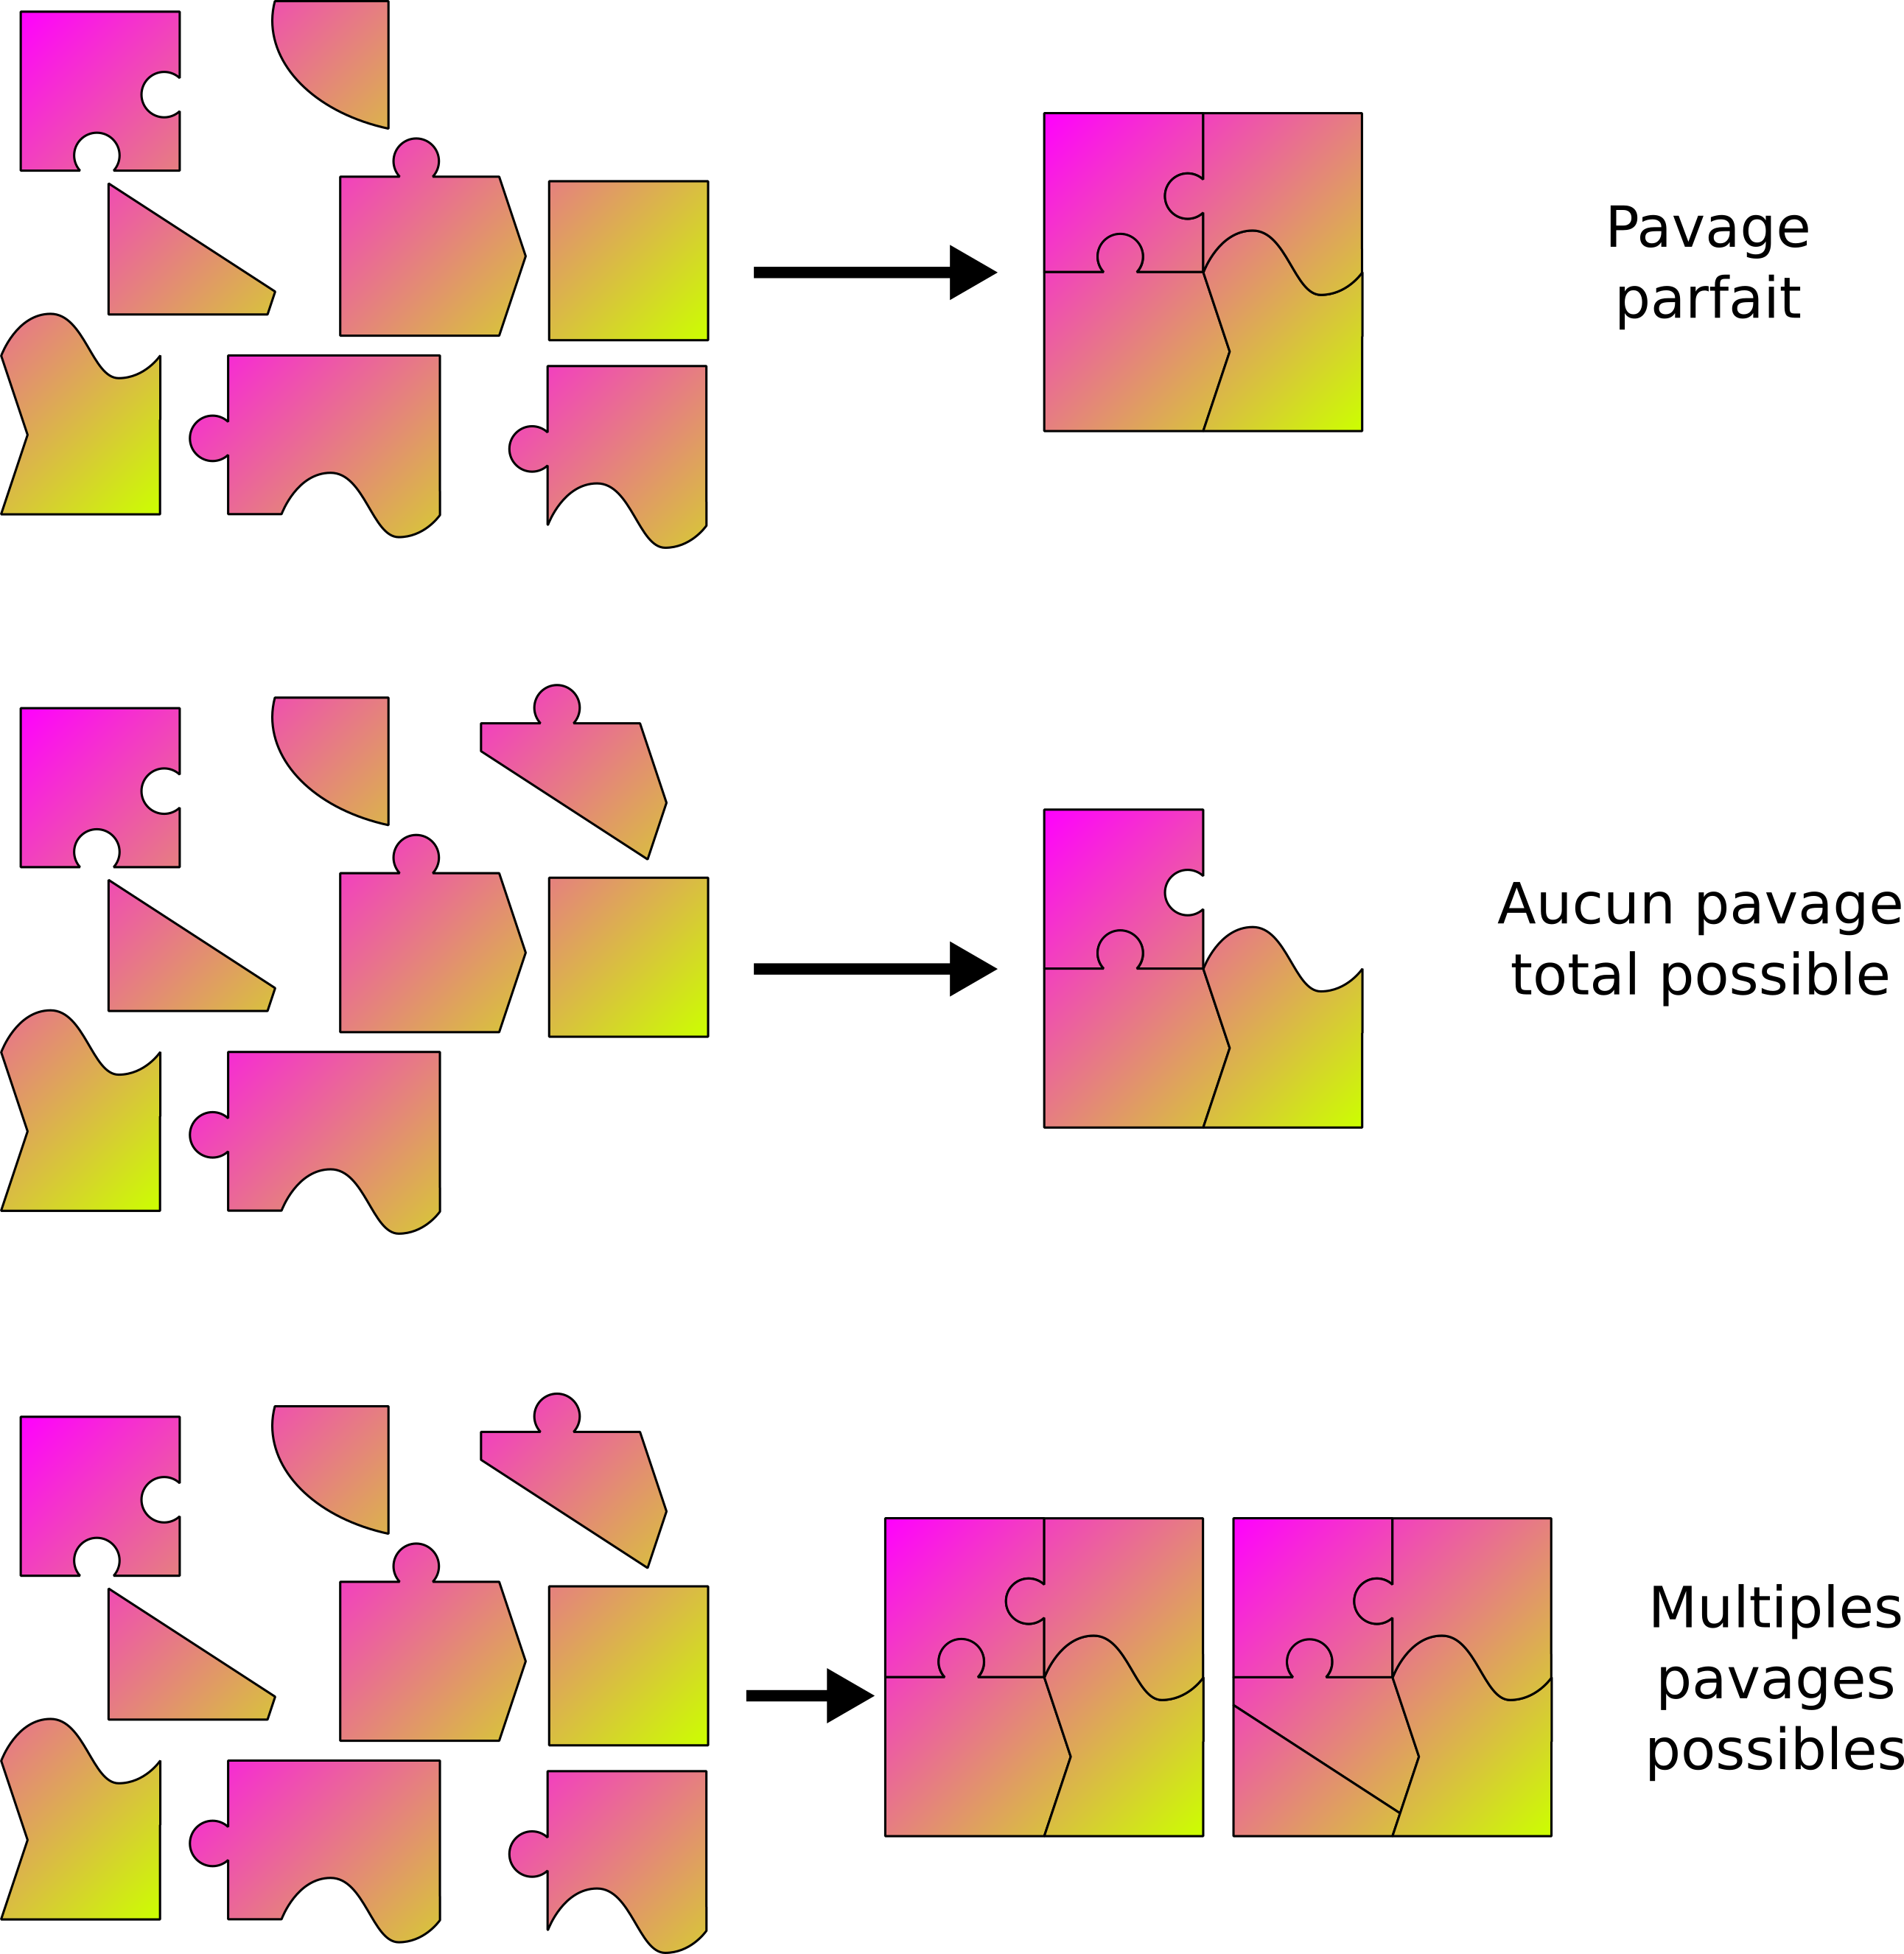
\includegraphics[width=300px]{Figures/s2m/pavage/couvertures.png}
    \caption{\label{puzzle_covs}Phase de pavage.
    Choix parmi toutes les pièces disponibles pour former le puzzle le plus grand possible}
  \end{center}
\end{figure}

Dans l'idéal, toutes les pièces nécessaires à la reconstruction du puzzle complet sont présentes dans l'ensemble des pièces trouvées (voir figure \ref{puzzle_covs}).
Dans le cas contraire, on ne peut pas reconstruire complètement le peptide à partir des résidus trouvés.
Dans ce cas, notre but sera alors de trouver un assemblage le plus complet possible.
Si beaucoup de résidus ont été trouvés lors de la première phase il est également possible que nous ne trouvions pas qu'une seule solution de reconstruction.
Nous n'aurons alors aucun moyen purement algorithmique de choisir quelle est la meilleure façon de découper ces peptides.




\subsubsection{Preuve de NP-Complétude}

\begin{figure}[!ht]
  \begin{center}
    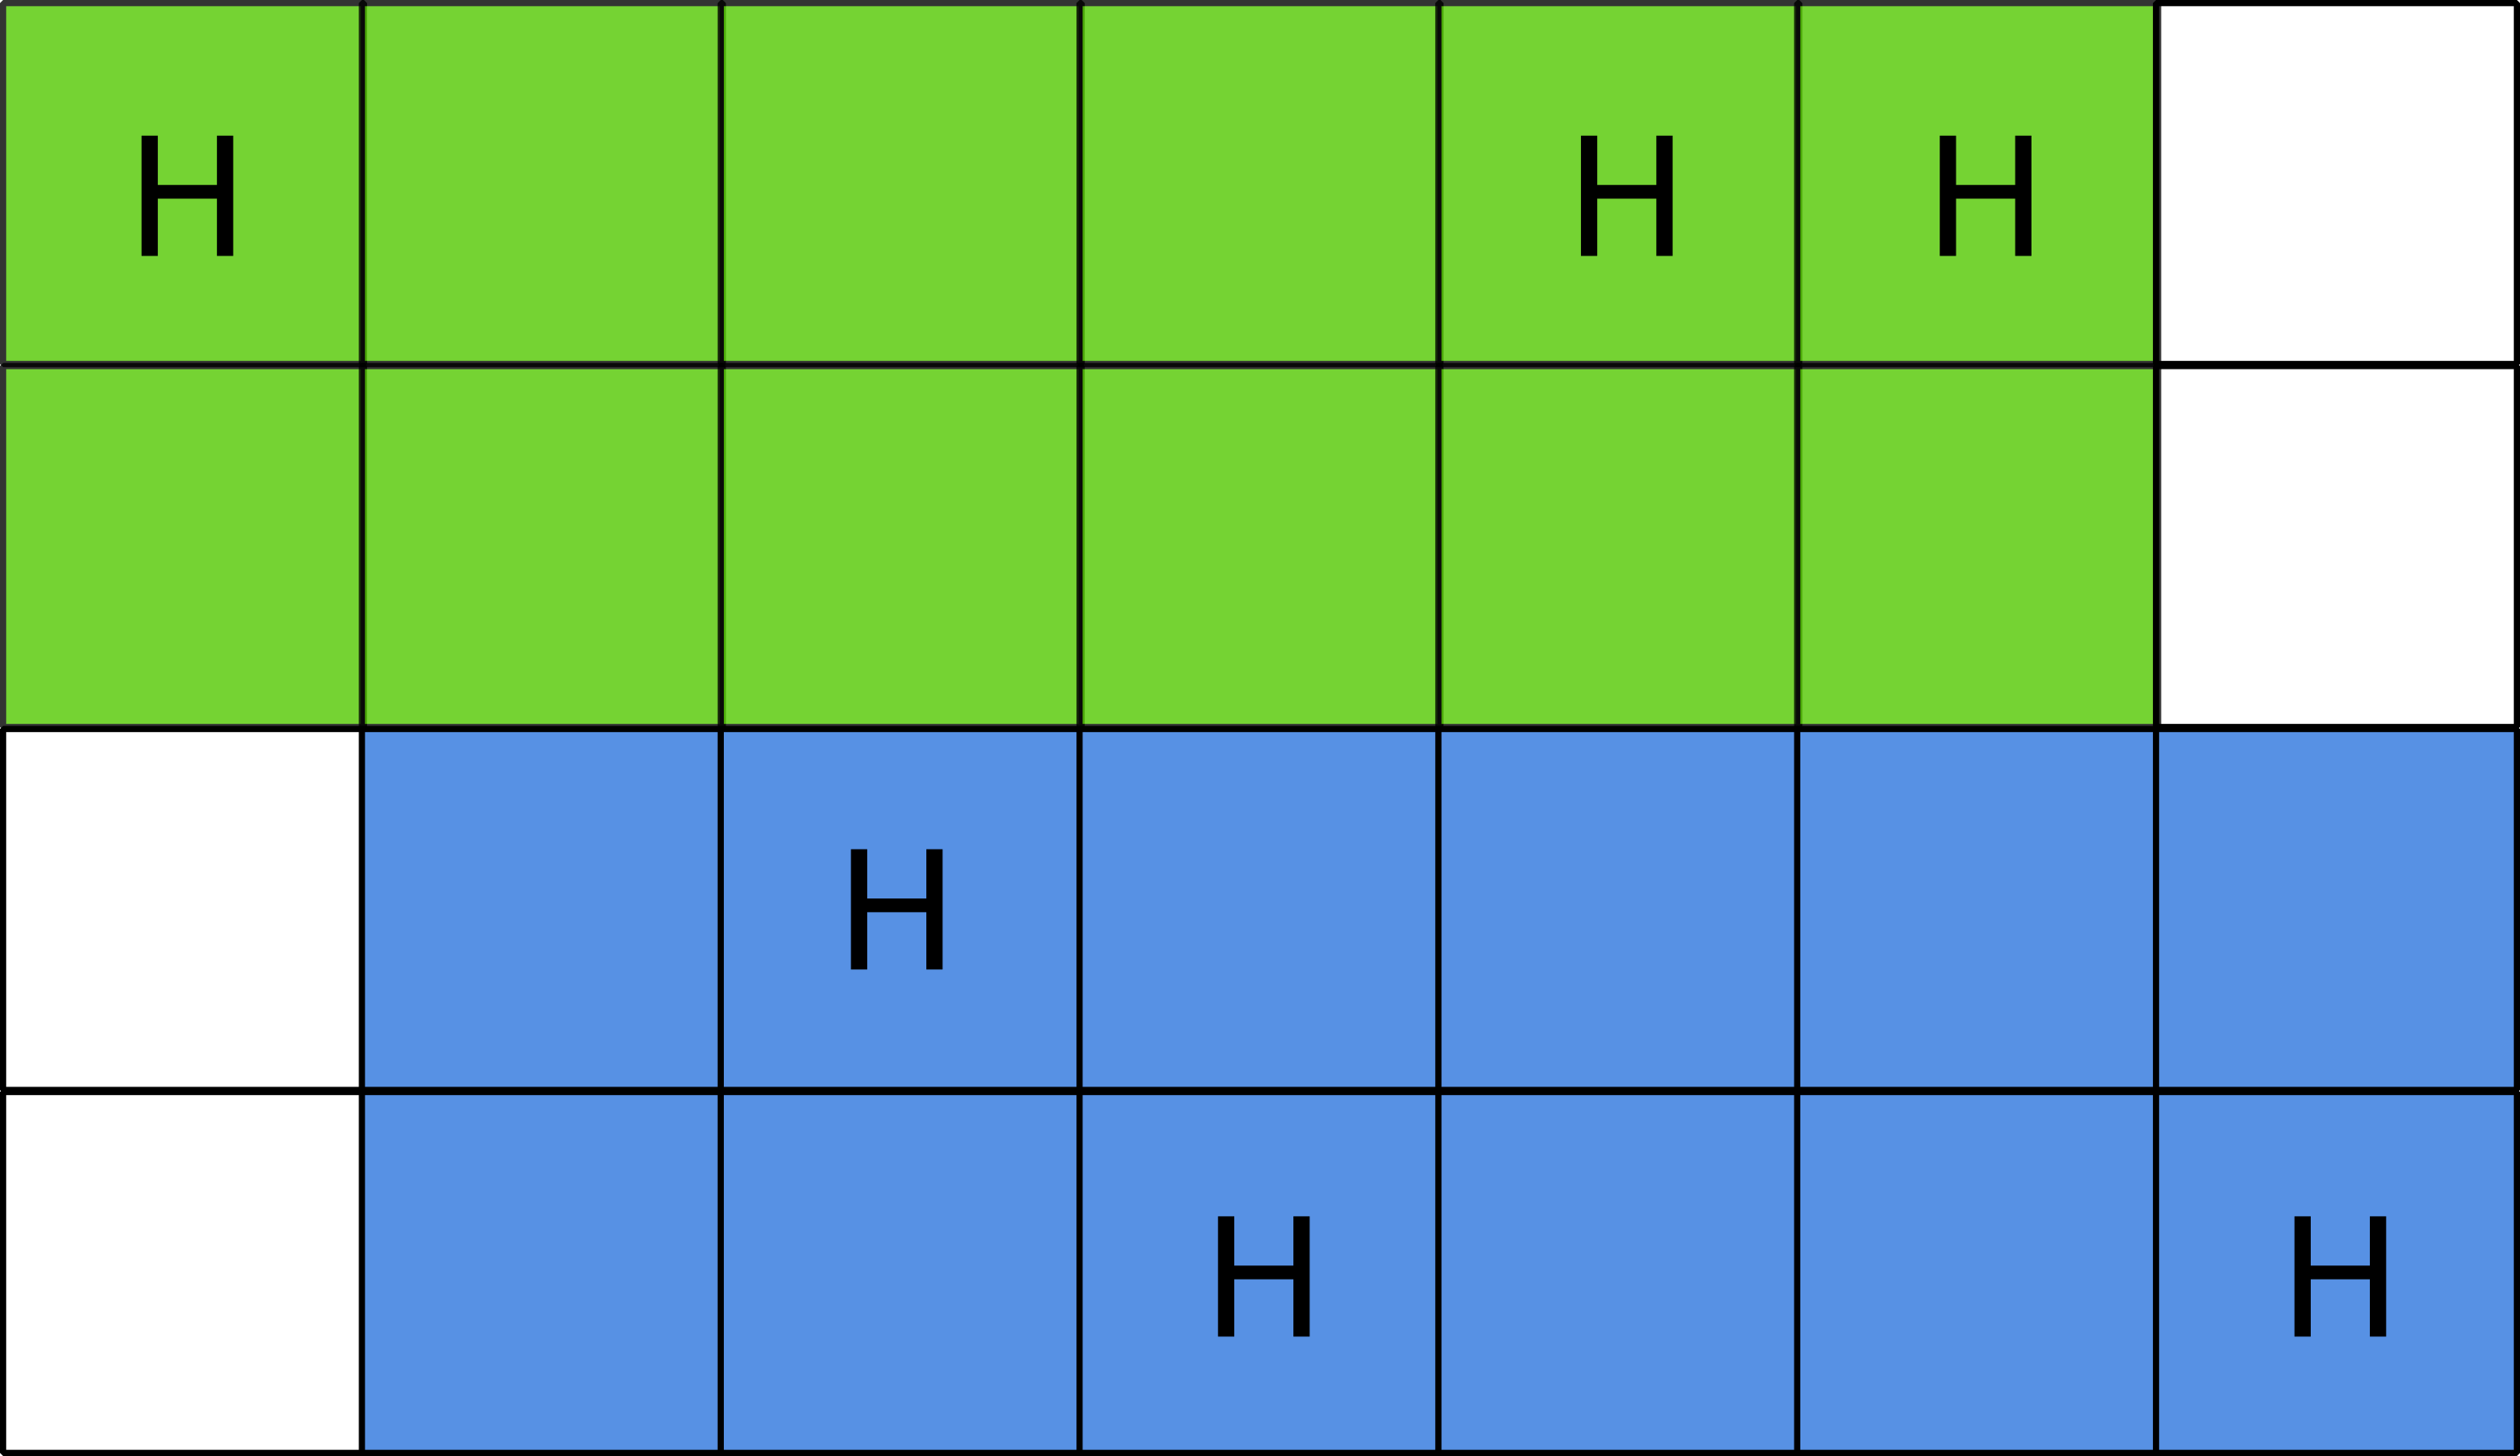
\includegraphics[width=250px]{Figures/s2m/pavage/pizza.png}
    \caption{\label{pizza}Exemple de pavage pour une pizza $7 \times 3$.
    Ici la pizza à atteint un pavage maximal avec les parts verte et bleu (24 / 28.}
  \end{center}
\end{figure}

En 2015, j'ai eu la chance de participer, avec mes amis Thomas Nachtergale et Alexandre Temperville, à la finale du concours d'algorithmique ``Google Hashcode''.
La veille de l'épreuve finale, un petit problème test nous a été proposé.
Le but était de découper une pizza (matrice), composée de cases de jambon (H dans la matrice) et de cases de sauce (T dans la matrice), en parts dites ``royales'', en minimisant le gâchis de pizza (morceaux de pizza exclus de toute part royale découpée) (voir schéma \cite{pizza}).
Les parts royales sont des parts rectangulaires contenant au minimum 3 cases de jambon et représentant une surface maximale de 12 cases.

Ce problème a été prouvé NP-Complet sur le forum stackexchange~\cite{de_biasi_complexity_2015} suite à la question d'un participant.
La preuve a été faite par réduction du problème ``Monotone cubic planar 1-3 SAT''.
Prouvons que le problème ``Pavage'' est également NP-Complet en utilisant une réduction du problème ``Pizza''.
Définissons ce problème Pavage comme le problème de décision suivant : Connaissant tous les monomères candidats au placement sur le peptide, est-il possible de trouver un sous ensemble de ces monomères qui soit non chevauchant et qui couvre 100\% du peptide ?

Premièrement, il est très facile de montrer par certificat que pavage est NP.
Le certificat contient l'ensemble des résidus pavés.
Leur nombre est borné par le nombre de résidus issus de l'isomorphisme.
Le certificat est donc de taille proportionnelle au problème.
Deuxièmement, le validateur de certificat doit vérifier qu'aucun résidu ne se chevauche.
Pour cela, il est possible de vérifier les chevauchements pour toutes les paires de résidus du certificat.
La vérification du certificat peut être faite de manière quadratique, ce qui permet de dire que le problème est NP.

Prouvons ensuite que nous pouvons résoudre le problème Pizza en utilisant le problème Pavage.
Codons donc Pizza dans Pavage~:
\begin{itemize}
	\item La pizza de taille $n \times m$ sera représentée par un peptide rectangulaire de taille $n \times m$.
	\item Chaque case de la pizza sera représentée par un atome qui ne pourra prendre les deux valeurs H et T selon le remplissage de la case.
	\item Le voisinage des cases sera représenté par des liens entre les atomes.
	L'atome correspondant à la case $(i,j)$ sera lié aux atomes correspondants aux case $(i-1,j)$, $(i+1,j)$, $(i,j-1)$ et $(i,j+1)$ (sauf sur les bords).
	\item Il possible polynomialement de générer toutes les parts réalisables sur une pizza (car leur taille maxiale est fixée).
	Chacune de ces parts sera représentée par un résidu placé sur le peptide comme si il avait été trouvé par l'étape de recherche de s2m.
	Par exemple une part allant de $(0,0)$ à $(2,3)$ sera représentée par un résidu couvrant tous les atomes entre ces coordonnées.
\end{itemize}

Avec ce codage, si nous arrivons à résoudre le problème de pavage, alors il devient alors possible de résoudre le problème de pizza.

Le problème de pavage est NP et il existe un problème NP-Complet qui peut se réduire en lui.
Pavage est donc NP-Complet.




\subsubsection{Pavage par optimisation linéaire}

\label{MIP_p}

\begin{figure}[!ht]
  \begin{center}
    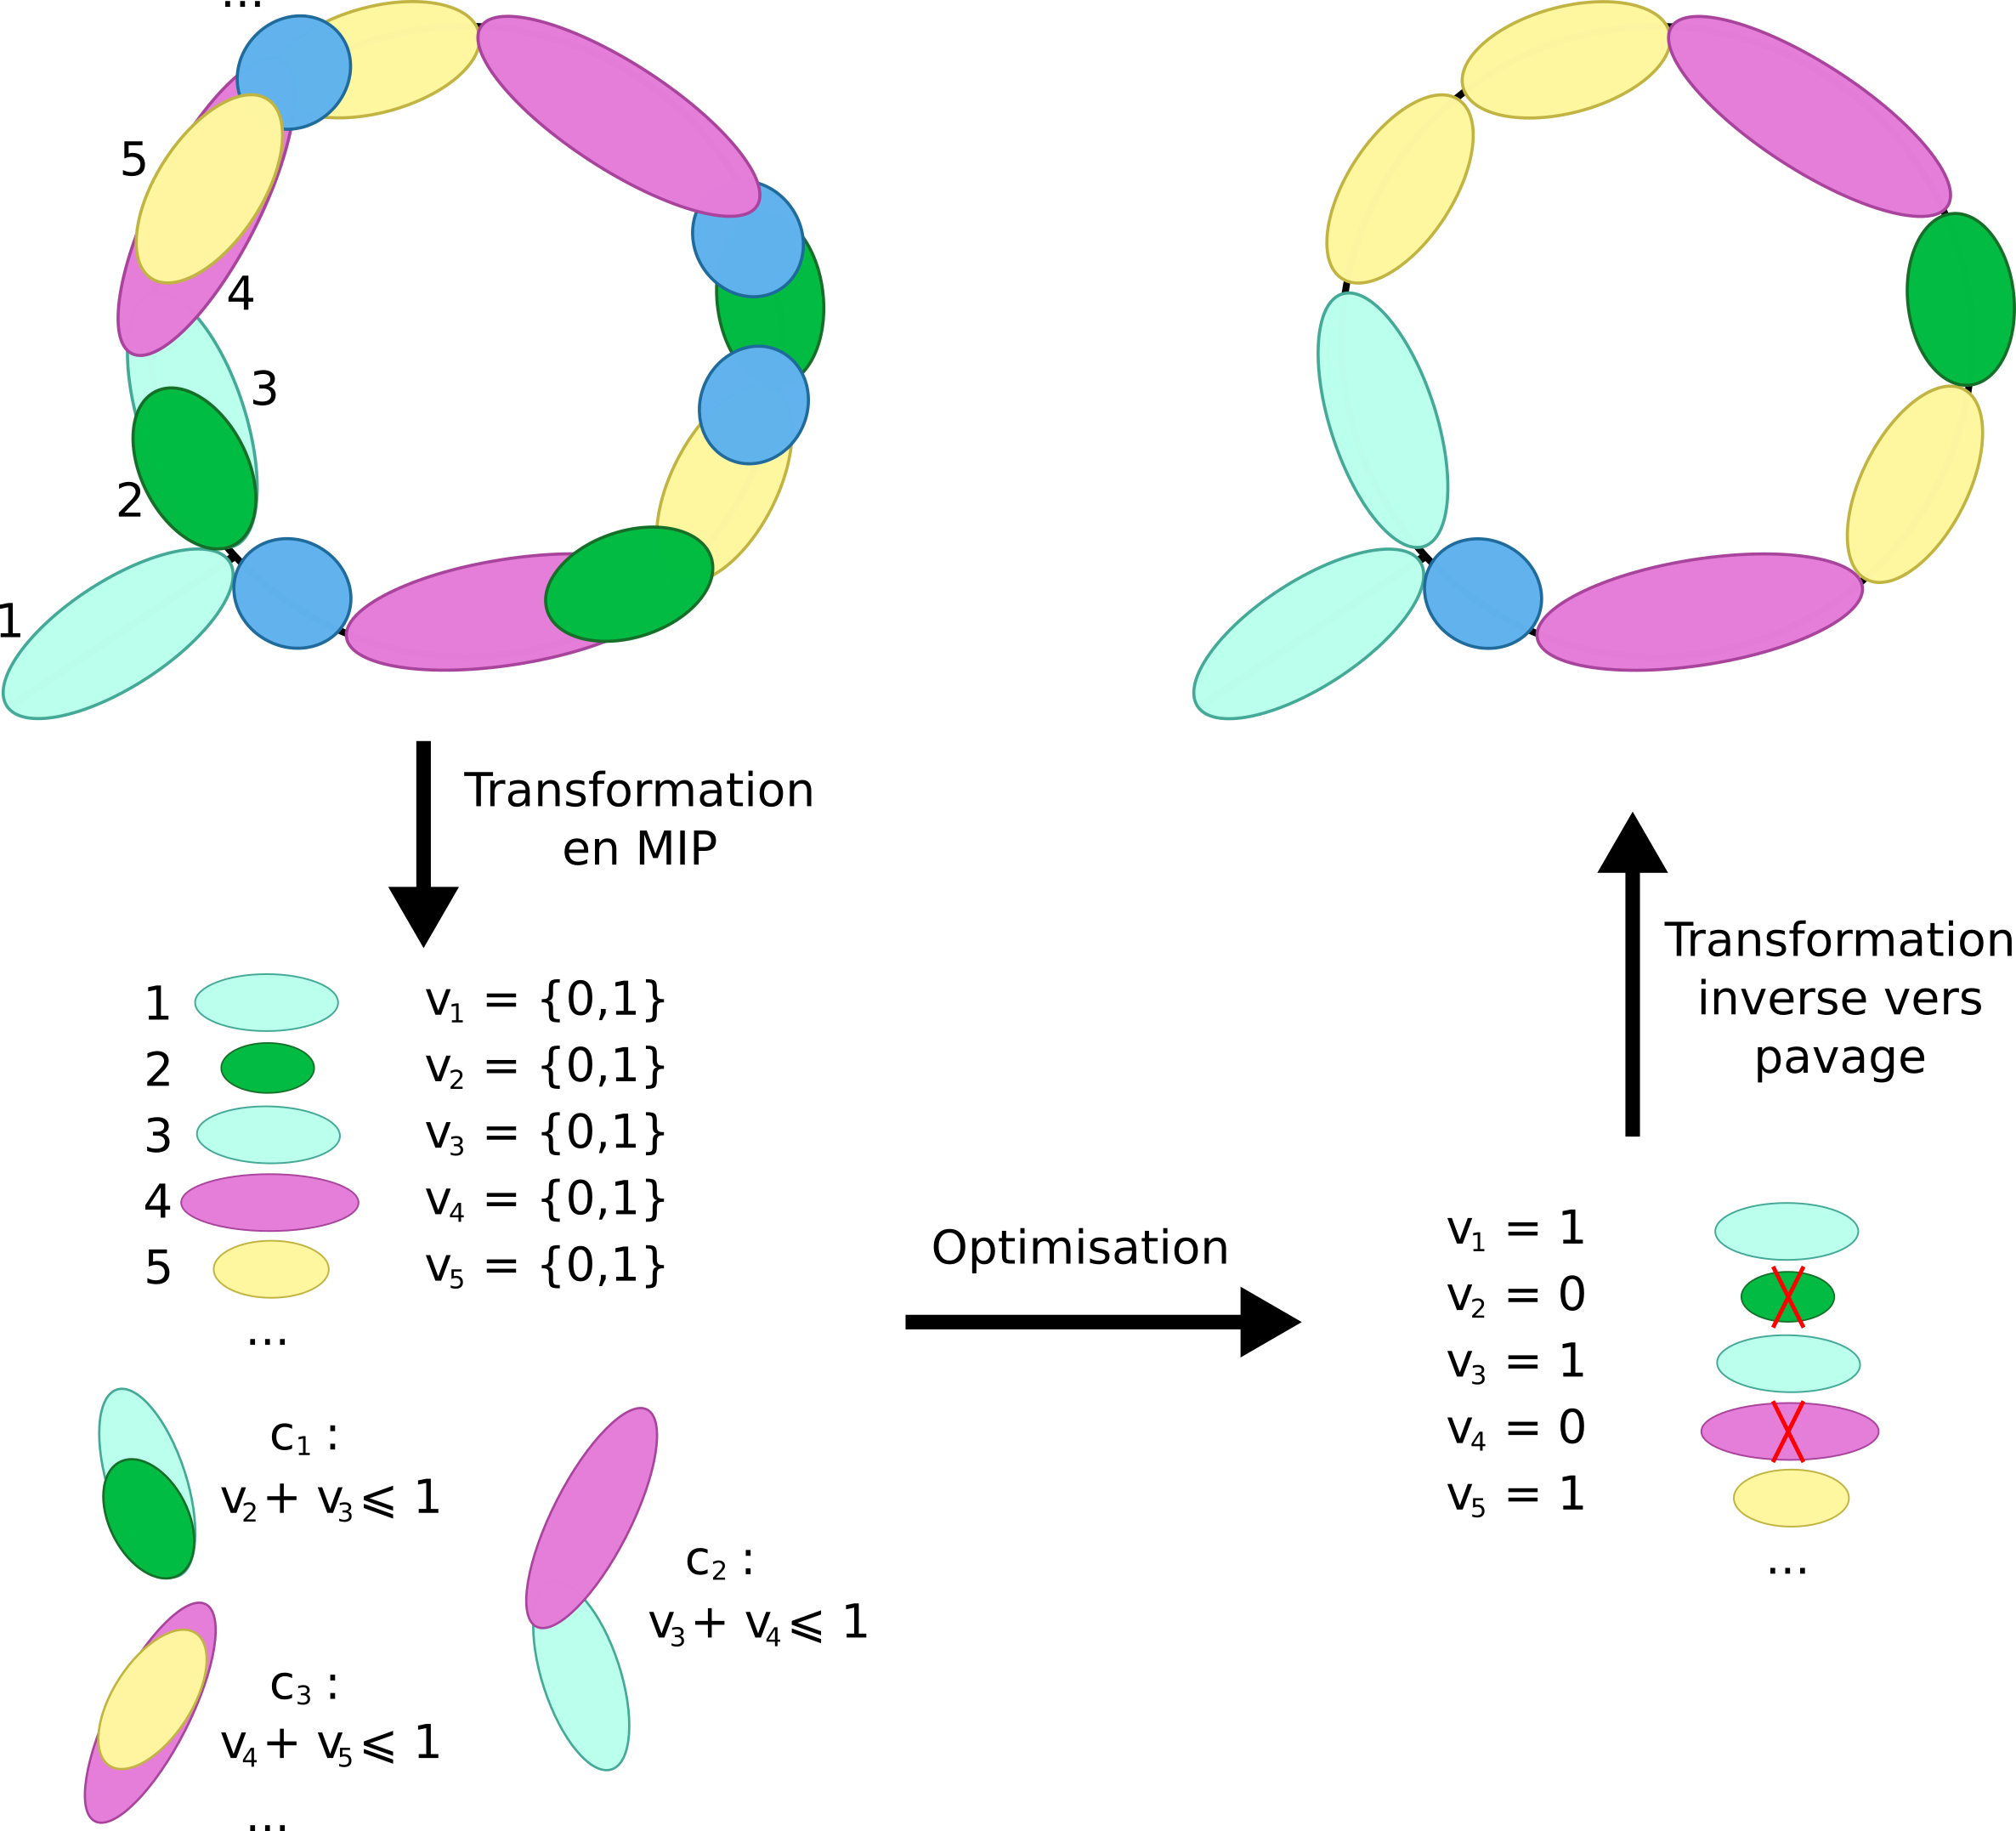
\includegraphics[width=350px]{Figures/s2m/pavage/MIP.png}
    \caption{\label{reduction}Représentation globale de la réduction du problème de pavage en MIP puis reconstruction de la
    solution}
  \end{center}
\end{figure}

Nous allons ici résoudre le problème de pavage de manière exacte par utilisation de la programmation linéaire (LP).
Un problème de programmation linéaire est un problème représenté par un ensemble de variables, une fonction de score ainsi qu'une liste de contraintes sur les variables.
La fonction de score est accompagnée d'un objectif de maximisation ou de minimisation.
Ce type de problème est classiquement résolu par l'algorithme du simplexe~\cite{murty_linear_1983}.
Depuis la publication, de nombreuses variantes de l'algorithme ont été créées.
L'une d'elle, appelée ``Mixed Integer Programming'' (MIP)~\cite{wolsey_mixed_2007}, permet de résoudre des problèmes pour lesquels les variables sont des entiers.

Dans notre cas, nous allons rechercher les résidus qui seront utiles pour notre assemblage final.
Ainsi, nous modélisons la présence ou l'absence dans la solution finale d'un résidu trouvé durant la première phase par une
variable binaire (0 pour l'absence et 1 pour la présence).

\begin{equation}
 \forall r_i, \quad \exists v_{r_i}, v_{r_i} \in \{0, 1\}
\end{equation}

où $r_i$ représente le i-ème résidu et $v_{r_i}$ la variable binaire correspondant à $r_i$.

Nous souhaitons également interdire la possibilité de chevauchement de deux résidus.
Nous pouvons caractériser cela par la restriction d'avoir au plus un résidu présent sur chaque atome (\textit{ie} une variable avec la valeur 1).
On obtient donc une contrainte pour chaque atome ; ces contraintes étant représentées par le fait que la somme de toutes les variables des résidus présents sur un atome ne peut être supérieure à 1.

\begin{equation}
 c_a : \sum_{r_i, a \in r_i} v_{r_i} \leqslant 1
\end{equation}

où $a$ est l'atome correspondant à la contrainte $c_a$.

Enfin, nous cherchons à maximiser le nombre d'atomes couverts par les résidus présents. La fonction de score sera
donc la somme des présences des résidus pondérée par la taille de chaque résidu :

\begin{equation}
 score : \sum^{r_i} v_{r_i} \times size(r_i)
\end{equation}

La réduction de notre problème de pavage en un MIP nous autorise l'utilisation des solveurs déjà existants pour trouver la solution exacte.
Nous pouvons par exemple utiliser la bibliothèque GLPK (l'une des seules bibliothèques de LP sous licence libre).

Bien que cette solution soit élégante, MIP dans sa version ne contenant que des variables binaires fait partie des 21 problèmes NP-complets de Karp~\cite{karp_reducibility_1972}.
Il n'existe donc actuellement aucune méthode de résolution de ce problème en temps polynomial.
Les cas les plus difficiles (ie contenant beaucoup de résidus chevauchants trouvés par isomorphisme) risquent de prendre beaucoup de temps.
Proposons également une heuristique rapide pour résoudre le problème.



\subsubsection{Pavage par heuristique gloutonne}

\label{TM_p}

L'un des moyen d'obtenir très rapidement une solution est de trier les résidus dans un ordre voulu puis de parcourir la liste triée en ajoutant le résidu courant à la solution uniquement si il ne chevauche aucun autre résidu de la solution.
On pourra toujours trouver au moins arrangement de la liste qui atteigne la solution optimale.
En faisant cela, nous reportons la difficulté du problème sur les critères de tri de la liste mais nous garantissons une très grande rapidité d'exécution.
Le but ici est de s'approcher de ce tri optimal en s'assurant d'une exécution très rapide de l'algorithme.


\begin{algorithm}[H]
  \caption{Algorithme de pavage glouton}
  \KwData{Un peptide requête $P$ et une liste de résidus $RES$ pavés sur $P$ lors de la phase d'isomorphisme}
  \KwResult{Un sous-ensemble de $RES$ de pièces non chevauchantes sélectionnées par l'algorithme glouton.}
  Soit $SOL$ un ensemble solution de résidus, initialement vide\;
  
  Trier $RES$ selon les critères gloutons\;
  \For {$r \in RES$} {
    \If {$r$ ne chevauche aucun $r'$ tq $r' \in SOL$} {
      Ajouter $r$ à $SOL$\;
    }
  }
  
  \KwRet $SOL$;
\end{algorithm}

Cet algorithme nécessite un tri sur une liste de $n$ résidus candidats ($O(n log n)$) puis consomme ensuite un élément de la
liste à chaque tour de boucle ($O(n)$). Contrairement à la résolution exacte présentée ci-dessus, si la fonction de comparaison
pour le tri ne dépendent pas de $n$ cet algorithme est polynomial.
Nous pouvons donc garantir la rapidité d'exécution si les critères de tri sont également calculable en temps polynomial.

Le but est d'opter pour l'efficacité maximale locale en espérant que l'efficacité globale sera également maximale.
Dans notre cas, la probabilité de trouver par hasard un résidu dans un peptide est inversement proportionnelle au nombre d'atomes qu'il contient.
On peut donc dire qu'un résidu est d'autant plus ``efficace'' que sa probabilité d'apparition par hasard est faible.
Le premier critère consiste donc à trier les résidus par taille décroissante (nombre d'atomes dont hydrogènes).
C'est un critère classiquement utilisé pour la résolution gloutonne du problème du sac à dos~\cite{_probleme_2016}.

\begin{figure}
  \begin{center}
    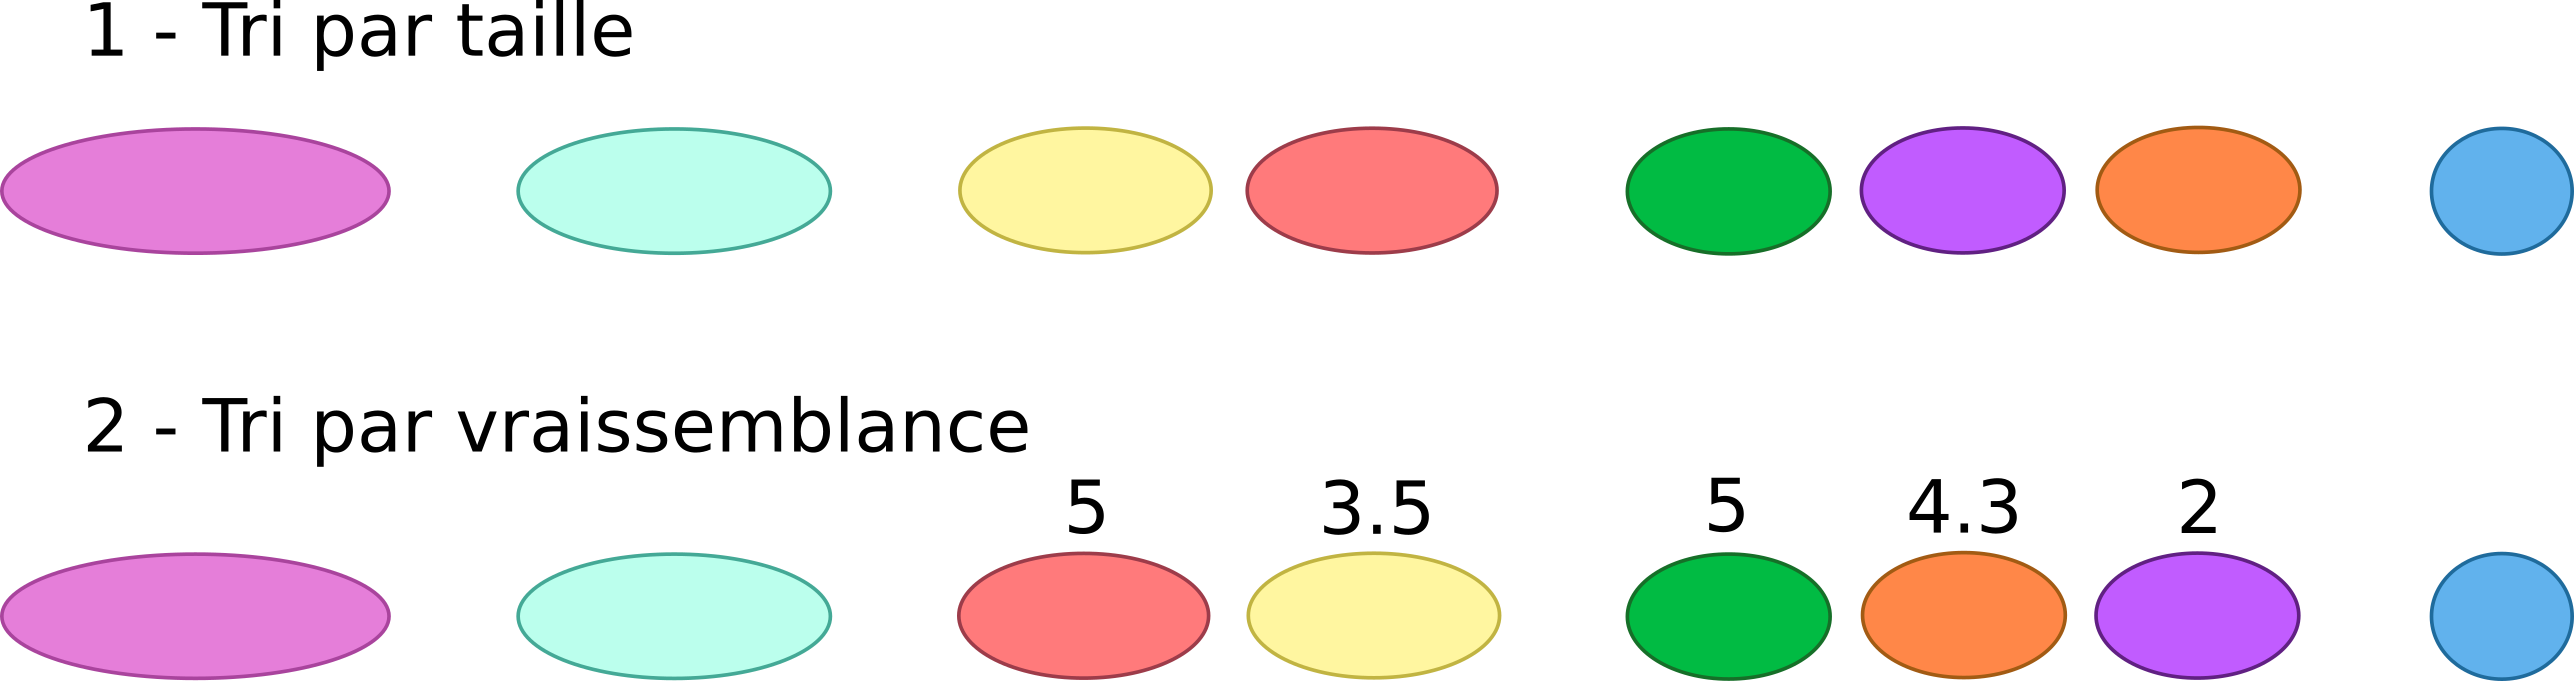
\includegraphics[width=400px]{Figures/s2m/pavage/tri.png}
    \caption{\label{tri_glouton}Tri pour le pavage glouton.
    Les résidus sont triés par taille puis par vraissemblance.}
  \end{center}
\end{figure}

Lorsque les résidus sont issus de monomères très similaires en taille, il arrive fréquemment que nombre d'entre eux
aient exactement le même nombre d'atome.
Dans ce cas, le critère de taille n'est plus suffisant pour le tri et il nous faut en ajouter d'autres.

En plus de leur taille, les résidus peuvent être caractérisés par leurs types de liaisons chimiques.
Chaque résidu forme des liens qui peuvent être différent d'un résidu à l'autre.
Certains liens apparaissent fréquemment alors que certains autres moins, ce qui nous permet en théorie d'estimer les
probabilités d'apparition d'un lien par rapport à un autre.
Ainsi, on peut considérer qu'un résidu contenant des liens qui apparaissent très souvent a plus de chance d'être le bon résidu
face à un second de même taille contenant des liens moins fréquents.
Cependant, nous ne possédons pas de statistiques sur les fréquences d'apparition des types de lien.

Pour tout de même pouvoir classer les résidus de cette manière, nous requérons l'expertise de l'utilisateur.
Avant la phase d'indexation, l'utilisateur doit définir les différentes règles de liaison qu'il veut voir apparaître dans les monomères.
C'est à ce moment que nous lui demandons également de remplir une valeur pour chacune de ces règles.
Cette valeur représente le poids que l'utilisateur souhaite donner à chacune des liaisons possibles.
Ce poids représente la confiance que l'on donne à l'apparition d'un type de liaison.
Ils nous permettent de calculer une valeur moyenne par liaison effectuée par le résidu.
Plus une moyenne sera élevée, plus la confiance en le résidu sera forte et donc plus il sera présent dans les premiers résidus du tri.

Dans le cas où plusieurs résidus ne peuvent être départagés lors du tri, nous considérons qu'ils sont équivalents et leur ordre sera aléatoire.


\subsubsection{Modulation de pavage}

Le pavage glouton est un très bon moyen d'obtenir un résultat rapidement, mais il ne garantit pas sa qualité.
Il possible que certains ``gros'' monomères aient pris la place de plus petits et que le pavage soit dans une impasse.
Dans ce cas, alors que la phase d'isomorphisme a identifié tous les monomères qui sont effectivement présents dans le peptide, le pavage correct n'est pas directement trouvé, l'algorithme nous laissant alors avec une solution partielle.
Lorsque qu'un cas de pavage incomplet se présente, nous pouvons donc nous demander s'il ne serait pas possible d'obtenir la solution complète avec les isomorphismes déjà effectués.
Nous proposons de repartir de la solution partielle et d'effectuer une recherche locale afin de nous convaincre qu'il n'est pas possible de faire mieux.

\begin{figure}[!ht]
  \begin{center}
    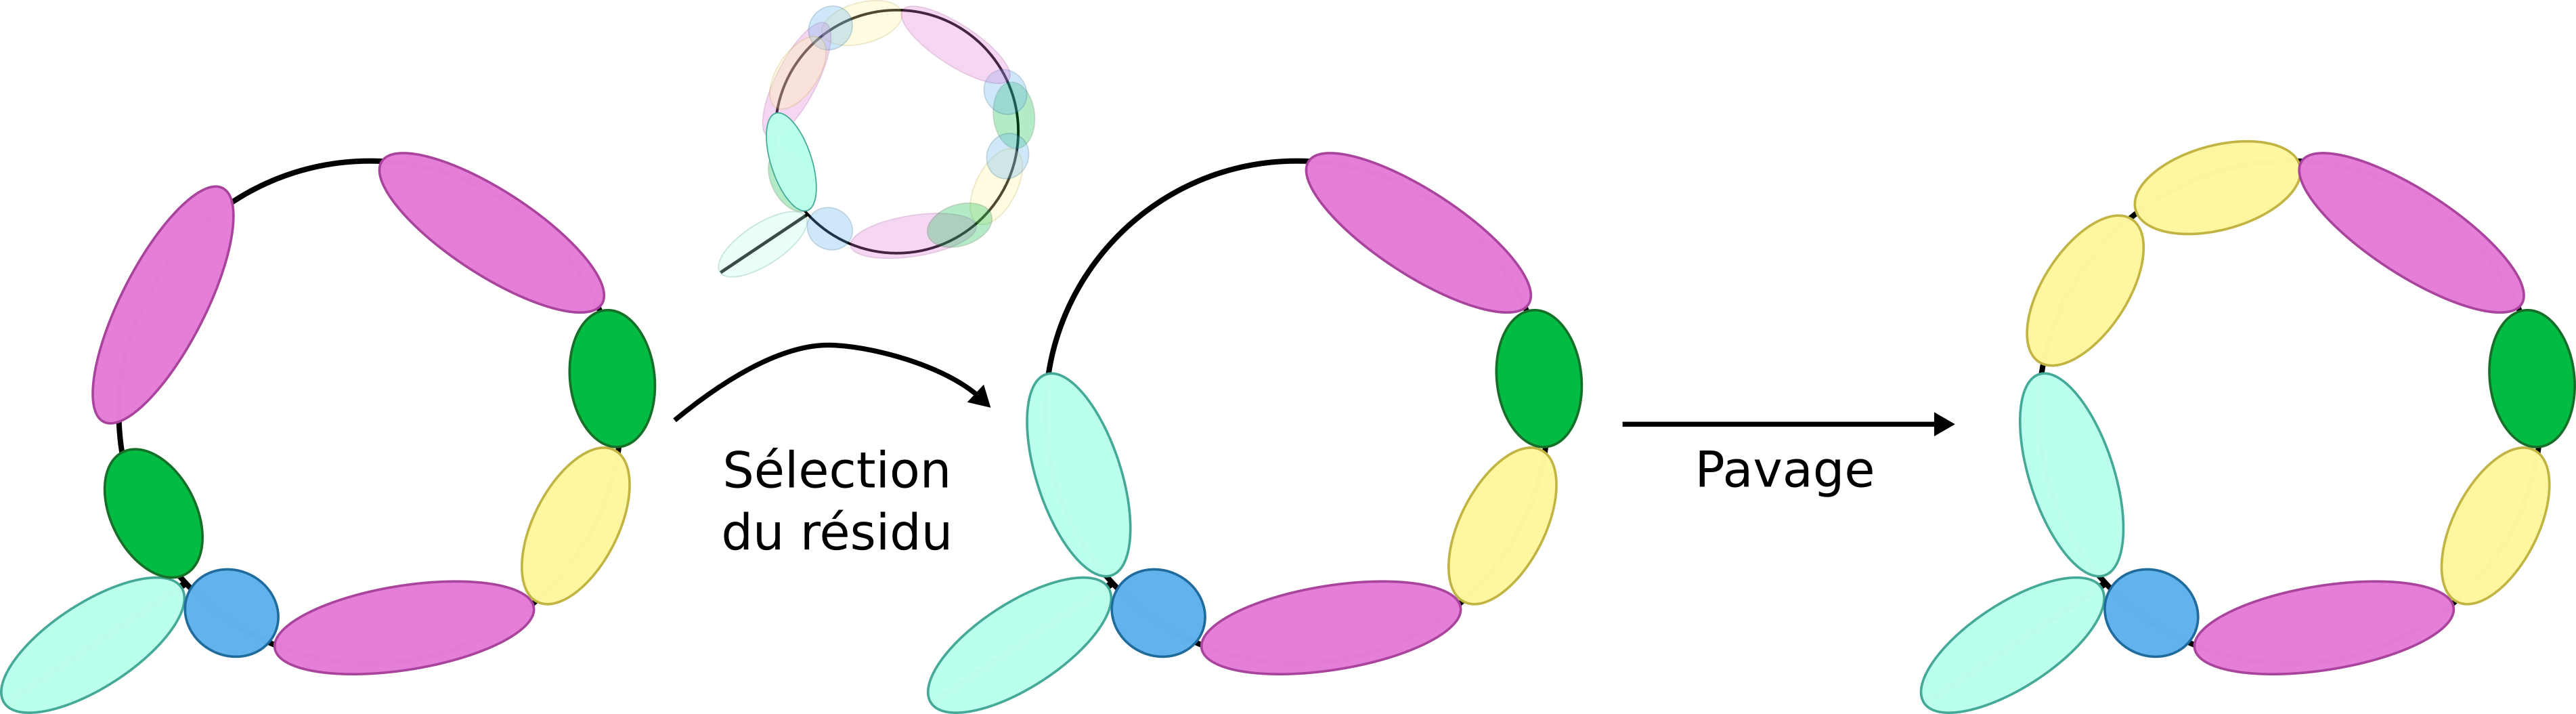
\includegraphics[width=450px]{Figures/s2m/pavage/modulation.png}
    \caption{\label{modulation}Représentation d'une étape de modulation.
    La première transition se fait par l'ajout forcé d'un résidu non choisi lors du pavage et de la suppression de tous les résidus le chevauchant.
    La seconde transition est effectuée par une étape de pavage glouton sur les zones non couvertes du peptide.
    Si une modulation ne suffit pas, cette étape est répétée de multiple fois au sein d'un algorithme de backtracking.}
  \end{center}
\end{figure}

L'algorithme de modulation que nous allons vous présenter permet d'être certain de passer par la meilleure solution si elle existe.
C'est un algorithme de backtracking classique qui passe par chacune des configurations possibles.
A chaque étape, l'idée est d'utiliser un résidu qui permet de couvrir une zone libre du peptide (qui a donc été écarté par le pavage précédent) et de l'ajouter au pavage (voir figure \ref{modulation}).
Utiliser ce résidu nous impose d'enlever de la solution les résidus chevauchants.
En priorisant les résidus non choisis du début de la liste triée utilisée par le pavage (voir \ref{TM_p}), nous essayons de trouver des solutions le plus rapidement possible.
Si la solution n'est pas complète à la suite de cet échange, nous relançons un pavage sur les zones laissées libres.
Après ce pavage, si la solution n'est toujours pas complète, nous relançons récursivement la modulation en interdisant de réutiliser les résidus que nous avons enlevé.
Enfin, si l'appel récursif ne parvient pas à une solution totalement couvrante, nous faisons marche arrière en changeant le résidu que nous avions choisi.

% 
% \begin{algorithm}[H]
%   \caption{Algorithme de modulation du pavage}
%   \KwData{Un peptide requête $P$ et une liste de résidus $RES$ pavés sur $P$ lors de la phase d'isomorphisme et triés par
%   l'algorithme glouton, une pré-solution $SOL$ et un ensemble $INT$ de résidus interdits d'utilisation.}
%   \KwResult{$SOL$, un sous-ensemble de $RES$ de pièces non chevauchantes sélectionnées par la modulation}
%   
%   $r \gets$ Premier élément de $RES$ couvrant au moins un atome non couvert et n'étant pas présent dans $INT$\;
%   \If {$r$ n'existe pas} {
%     \KwRet Impossible\;
%   }
%   Soit $SUPPR$ une liste de résidus\;
%   \For {$r_i \in SOL$} {
%     \If {$r_i$ chevauche $r$} {
%       Ajouter $r_i$ à $SUPPR$\;
%       Supprimer $r_i$ de $SOL$\;
%       Ajouter $r_i$ à $INT$\;
%     }
%   }
%   
%   Lancer un pavage pour compléter $SOL$\;
%   
%   \If {$SOL$ couvre $P$ à 100\%} {
%     \KwRet $SOL$\;
%   }
%   
%   $SOL \gets$ Modulation récursive\;
%   
%   \If {$SOL = $ Impossible} {
%     Supprimer $r$ de $SOL$\;
%     Ajouter $r$ dans $INT$\;
%     \For {$r_i \in SUPPR$} {
%       Enlever $r_i$ de $INT$\;
%       Ajouter $r_i$ à $SOL$\;
%     }
%   }
%   
%   \KwRet $SOL$\;
% \end{algorithm}


L'algorithme permet d'explorer toutes les solutions possibles jusqu'à obtenir la meilleure.
Le problème majeur est que si une solution parfaite n'existe pas, l'algorithme de modulation va parcourir tout l'arbre des solutions et l'exécution ne sera pas plus rapide que l'exécution d'une résolution de MIP.
Rappelons que le pavage glouton effectue des choix que nous supposons pertinents.
Il n'est donc normalement pas nécessaire de modifier la solution en profondeur pour obtenir l'idéal.
Si la solution n'est pas trouvée rapidement, il y a fort à parier que la solution idéale n'existe pas.
On peut donc limiter la profondeur de notre algorithme de modulation limitant la profondeur de la récursion.
Cette limite de profondeur diminue fortement le temps de calcul mais ne garantit plus de passer par l'optimal.
Cependant, si une solution n'est pas trouvée en quelques étapes de modulation, il est fort probable qu'aucune solution ne soit possible.


\subsection{Recherche approximative (light)}

\label{light_p}

\begin{figure}
  \begin{center}
    \includegraphics[width=300px]{Figures/s2m/residues/tautomers.png}
    \caption{\label{tautomer}Tautomérie d'une molécule}
  \end{center}
\end{figure}

Suite à des variations de composition ou de structure survenant dans certains résidus quelques polymères ne sont pas découpés correctement en utilisant les algorithmes précédents.
Il y a essentiellement deux cas pour lesquels l'isomorphisme ne fonctionne pas.
Le premier cas concerne un \textit{monomère ionisé} au sein du peptide, c'est-à-dire lorsqu'un proton a été perdu.
Ainsi, lors de la phase d'isomorphisme, la fonction de comparaison d'étiquettes ne répond plus correctement car il manque un $H$ sur l'un des atomes.
Dans le second cas, c'est encore l'isomorphisme qui ne reconnaît pas un résidu car celui-ci est intégré sous un variant tautomérique (voir figure \ref{tautomer}).
Un tautomère de molécule est un isomère structurel de cette molécule.
C'est à dire que la molécule tautomérique contient l'ensemble des atomes de la molécule initiale  mais certains de ces atomes ne sont plus liés aux mêmes voisins.
Dans le cas d'un tautomère, c'est un noyau d'hydrogène qui se déplace et change de voisin.
Cette charge positive déplacée est compensée par une charge négative qui se déplace dans l'autre sens.
Ce déplacement d'électron se concrétise par le déplacement d'une liaison double.
Ce déplacement peut même avoir lieu entre deux résidus différents d'un peptide.

\begin{figure}[!ht]
  \begin{center}
    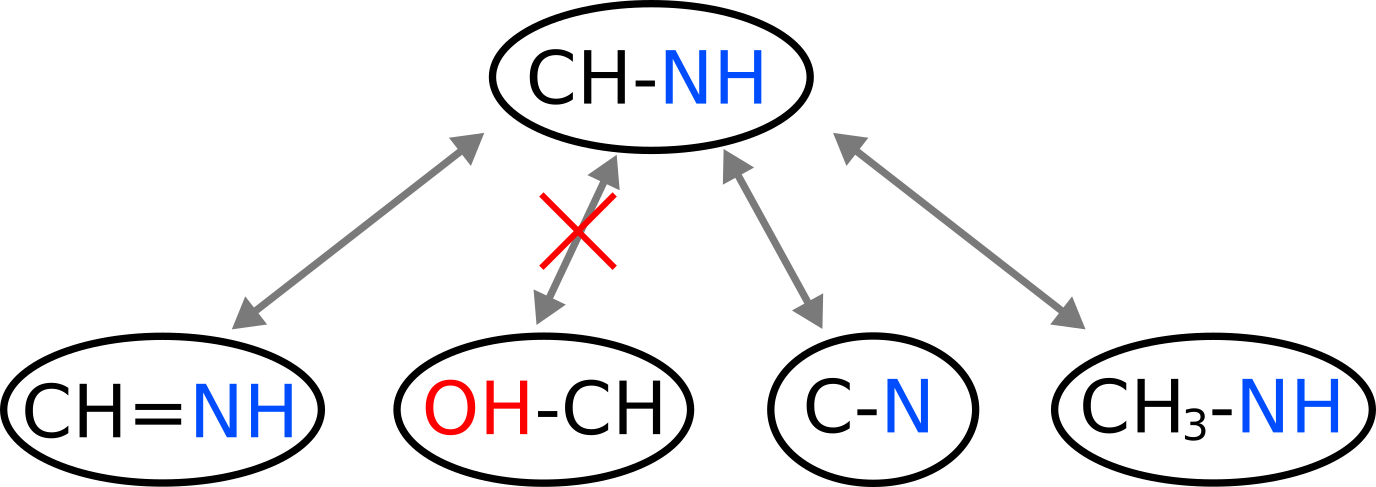
\includegraphics[width=200px]{Figures/s2m/recherche/light.png}
    \caption{\label{label_matching}Exemple de fonctionnement de la fonction de matching ligth d'étiquettes.
    Puisque le nombre d'atomes d'hydrogène n'est plus un critère sélectif et que l'arité de la liaison chimique non plus, la comparaison est valide dès que les deux atomes non hydrogène sont identiques.}
  \end{center}
\end{figure}

Les deux transformations présentées ont pour point commun de ne pas modifier en profondeur la structure des molécules.
Dans les deux cas seuls les ``décorateurs'' des étiquettes sont modifiés (hydrogènes et arité de liaison).
Le moyen simple de reconnaître ce type de molécule est alors d'oublier ces décorateurs lors de la phase d'isomorphisme (voir figure \ref{label_light}).
Dès lors les résidus sont reconnus quel que soient leurs variations sur les hydrogènes ou les liens.
% Cette modification ne fait pas varier la qualité des résultats sur les NRP car les monomères utilisés diffèrent entre eux au delà des atomes d'hydrogène.
Bien que très séduisante cette méthode pose un problème de temps de calcul.
La plupart des monomères NRP ne contiennent que des atomes C N O et H.
Ne pouvant plus utiliser les H comme décorateurs et en rendant les liens indifférents les uns des autres, le nombre d'étiquettes différentes chute à 9.
Il est donc compréhensible que le temps de calcul augmente en conséquence.

La solution est une nouvelle fois hybride.
Dans un premier temps, nous cherchons rapidement une solution en effectuant un
isomorphisme contenant toutes les étiquettes (isomorphisme {\em strict}), puis en effectuant un pavage.
Dans un second temps si aucune solution complète n'est trouvée, nous relançons le processus en commençant par
une nouvelle phase d'isomorphisme sans les décorateurs (isomorphisme \textit{light}).
Cette seconde phase d'isomorphisme est effectuée localement autour des zones qui ont posé problème lors du premier tour de 
l'algorithme.
Cet algorithme en deux temps traite rapidement tous les cas simples avec des sous algorithmes efficaces, pour revenir ensuite sur les cas les plus difficiles avec des algorithmes plus sensibles.

\subsection{Vue globale des algorithmes}

\begin{figure}
  \begin{center}
    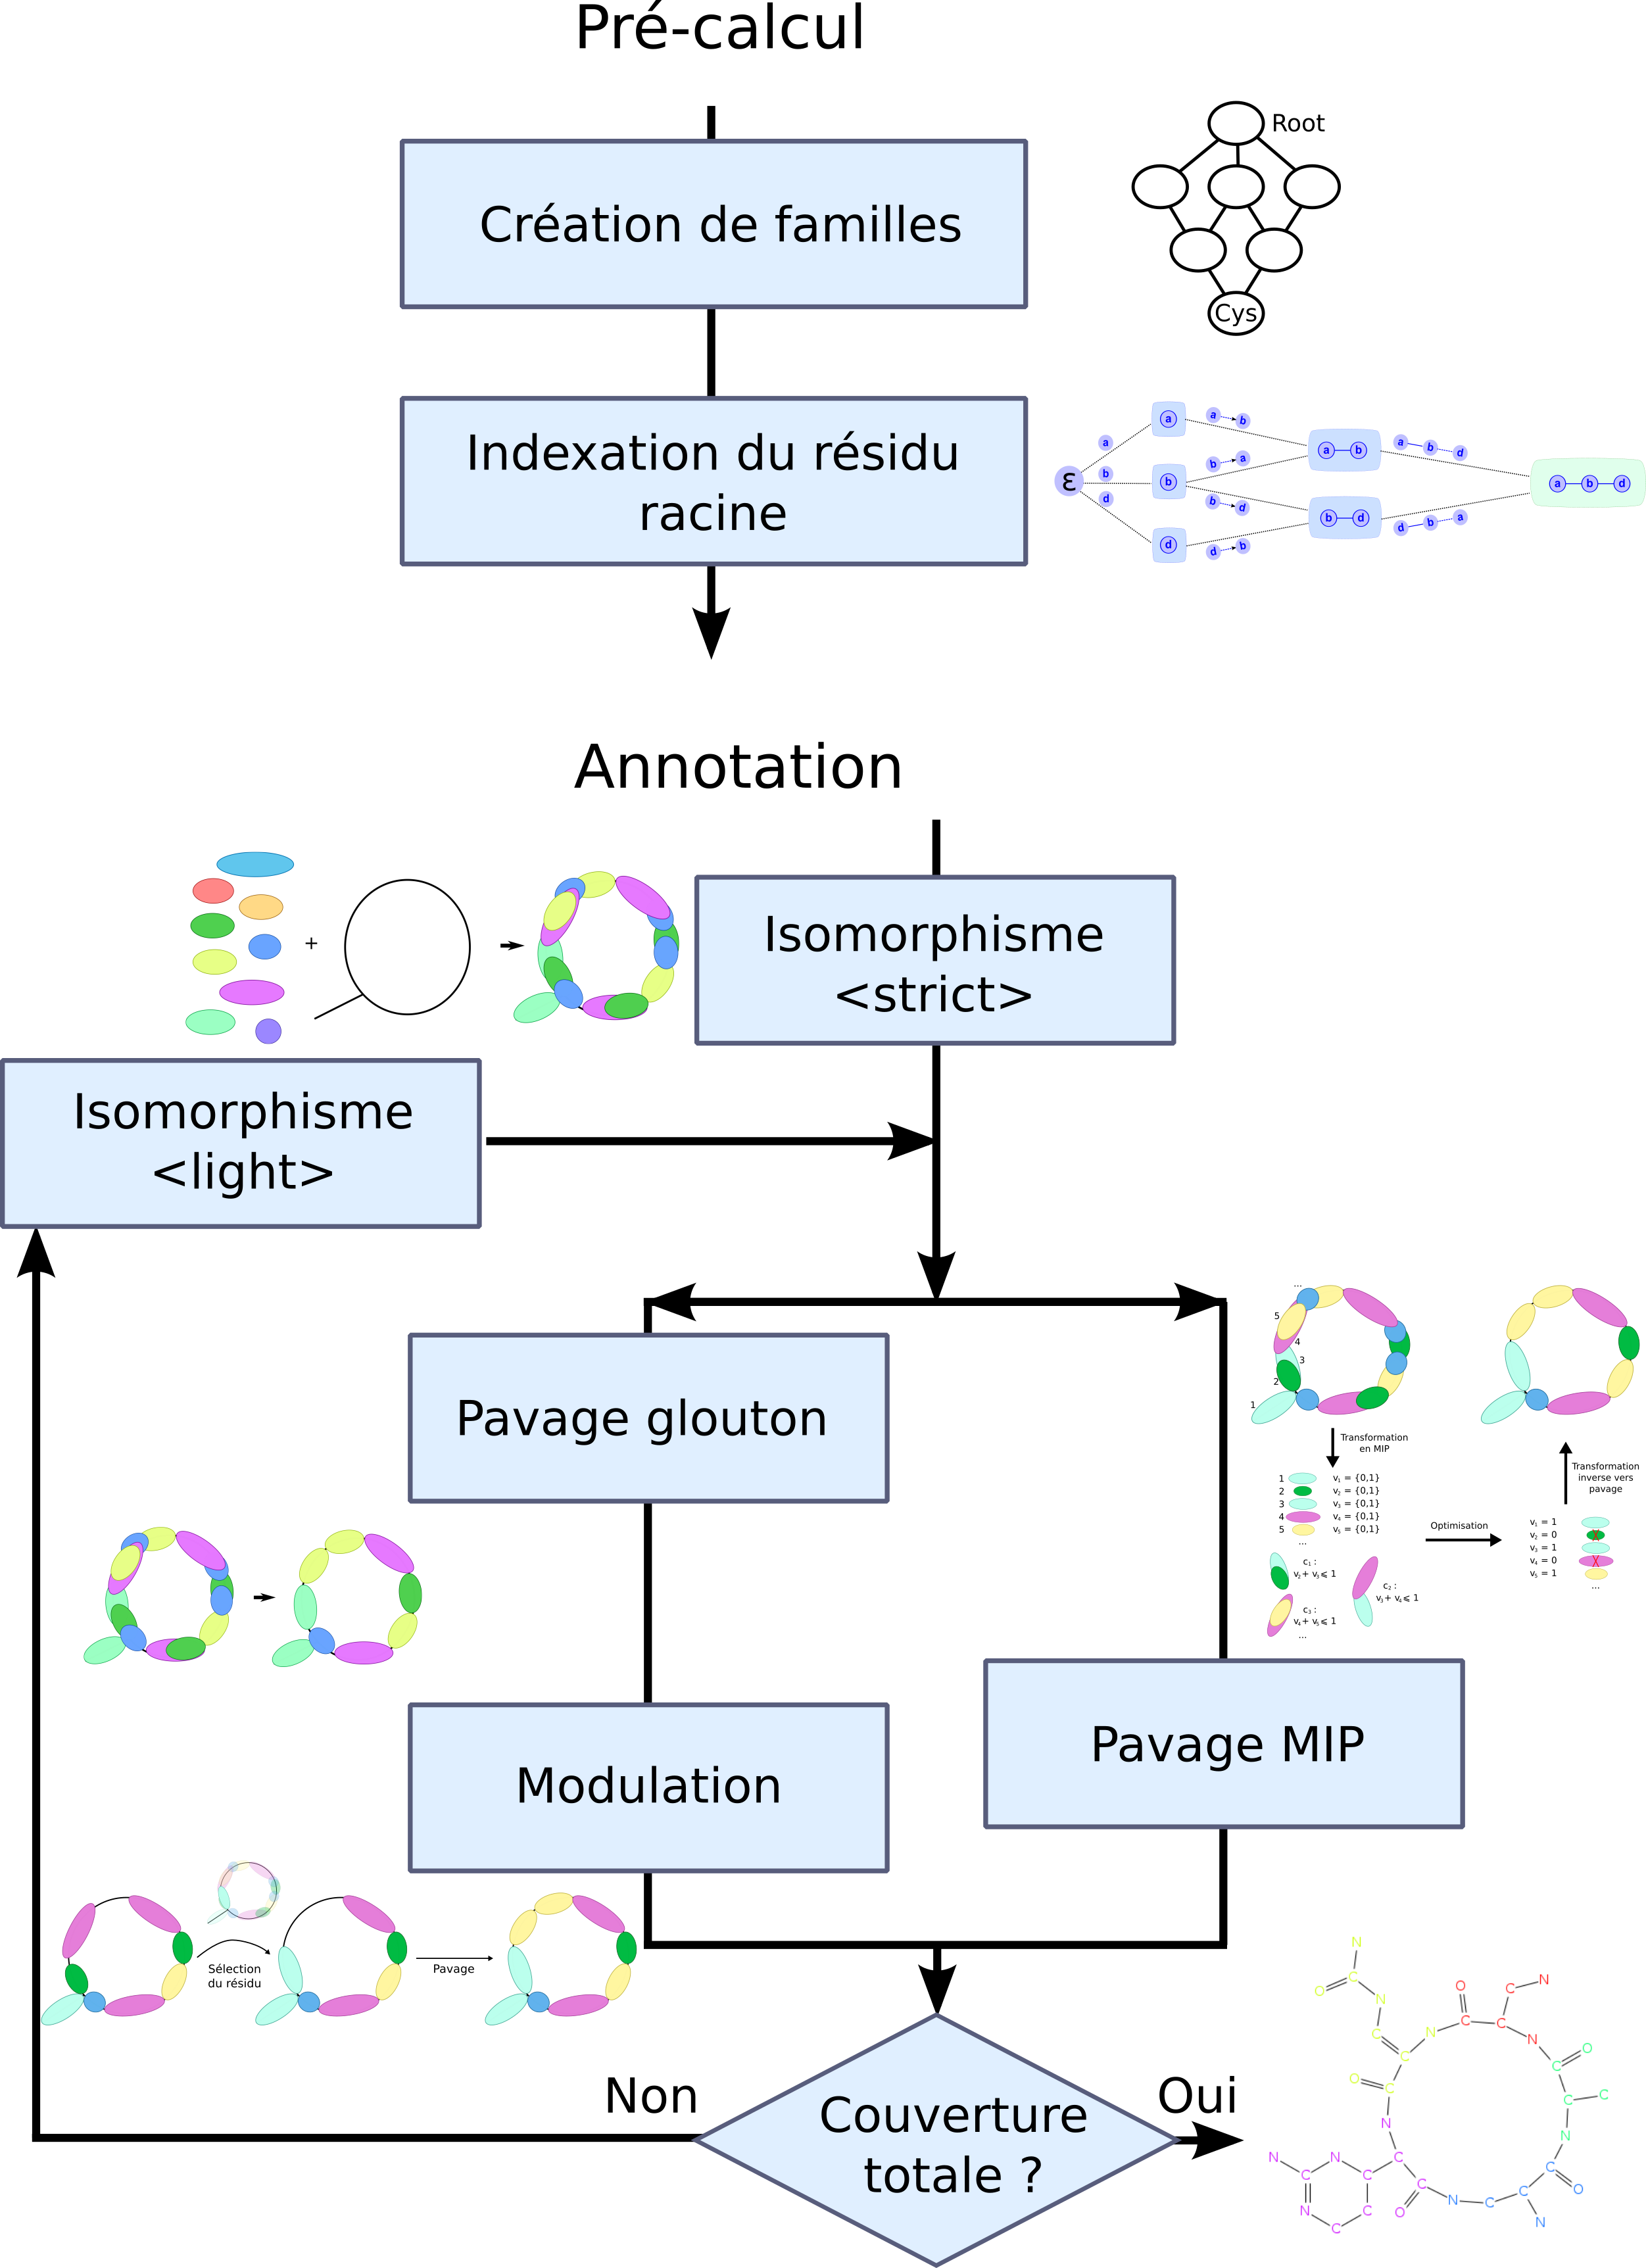
\includegraphics[width=450px]{Figures/s2m/algorithms.png}
    \caption{\label{global_s2m}Schéma global de Smiles2Monomers}
  \end{center}
\end{figure}

Tout au long cette partie, nous avons présenté par étapes les différentes parties de s2m.
Nous rassemblons ici tous les étapes au sein d'un schéma global (figure \ref{global_s2m}).
La première partie du schéma (au-dessus des pointillés) est composée des deux phases de pré-calcul (voir \ref{index_p}).
Cette étape de pré-calcul est gourmande en temps et mémoire mais n'est à effectuer qu'une seule fois.
Chacune des deux phases de cette étape se déroule en temps exponentiel mais reste calculable grâce à la petite taille des
données.
La partie principale de s2m possède deux alternatives algorithmiques.
Dans les deux cas, l'algorithme commence par une phase de recherche d'isomorphismes (voir \ref{isomorphisme_p}) afin de connaître les résidus candidats à la composition du polymère.
Ensuite vient la phase de pavage, effectuée soit par une résolution de MIP (voir \ref{MIP_p}), soit par une heuristique de pavage (voir \ref{TM_p}).
Enfin, pour les cas plus difficiles, nous effectuons plusieurs passes de recherche d'isomorphismes \textit{light} (voir \ref{light_p}) suivis par de nouvelles phases de pavage et modulation.

L'algorithme global est paramétrable.
Pour le précalcul, nous pouvons fixer la variable $k$ qui définira la taille de chaine calculée avec le modèle markovien.
Nous rappelons encore une fois que cette taille n'aura pas d'influence sur le résultat, mais uniquement sur le temps de calcul.
Pour la partie recherche, nous devrons choisir le nombre de fois où nous effectuerons l'isomorphisme \textit{light}''.
Ce paramètre est appelé ``retry'' dans le logiciel (nombre de fois où l'on ré-exécute la boucle).
Si nous optons pour la méthode heuristique de modulation, il est également nécessaire de définir une profondeur maximale de modulation (paramètre appelé ``modulation'' dans le logiciel).
L'influence de ces paramètres sur l'exécution de l'algorithme sera étudiée au sein de la section \ref{parameters_choice}.




\section{Résultats et interprétations}

\label{res_int}

\subsection{Jeux de données}

\subsubsection{Les constituants des jeux de données}

Nous souhaitons connaître la pertinence des annotations issues de s2m.
Pour cela, nous avons construit deux jeux de données tests, au sein desquels les annotations attendues sont déjà connues.
Ces bases de test sont composées de polymères comprenant à la fois leur SMILES (représentation de leur structure atomique) ainsi que l'annotation attendue (graphe monomérique).
Sans la structure atomique, nous ne pouvons pas lancer s2m et sans structure monomérique, nous ne pouvons pas tester les résultats.
Il existe très peu de bases de données contenant ces deux informations à la fois.
Les bases Norine et CCD que nous allons présenter ici sont les seules, à notre connaissance, à posséder une grande quantité de polymères contenant ces deux structures.

Pour les entrées de s2m, nous constituons une base de monomères pour chacun des jeux de données.
s2m pré-calculera les indexes pour chaque base de monomère puis s'exécutera sur chaque polymère.
L'annotation de sortie sera alors comparée à l'annotation préexistante pour en définir la qualité.


\subsubsection{Premier jeu de données : Norine}

Puisque le déclenchement de ce travail est dû à la volonté d'accroitre le nombre d'annotations de NRP dans Norine, le premier jeu de données sera logiquement constitué de polymères non ribosomiques déjà annotés issus de cette base.
Toutes les entrées de Norine sont accompagnées d'annotations monomériques et c'est d'ailleurs ce qui fait la force de cette base.
Nous avons donc extrait tous les NRP pour lesquels un SMILES était renseigné pour constituer un jeu de polymères tests.
La base de monomères est quant à elle constituée de l'ensemble des monomères connus et présents dans Norine.


%Citations :
%· The chemical component dictionary: complete descriptions of constituent molecules in experimentally determined 3D macromolecules in the Protein Data Bank
%· The Protein Data Bank
\subsubsection{Second jeu de données : The Chemical Component Dictionary (CCD)}

CCD~\cite{westbrook_chemical_2015} est une sous partie de la base de données PDB~\cite{berman_protein_2000} (Protein Data Bank).
Cette base regroupe toutes les petites molécules présentes dans PDB.
Parmi celles-ci se trouvent de nombreux polymères annotés ainsi que les monomères les constituant.
L'avantage de cette base est que toute molécule y étant présente est accompagnée de son SMILES.
En extrayant les molécules annotées comme polymères, nous avons constitué un second jeu de données.
Pour constituer la base de monomères dont s2m à besoin en pré-traitement, il nous a suffit d'extraire les molécules présentes dans les annotations polymériques.


\subsubsection{Résumé sur les données}

Les données de validation seront composées de deux jeux distincts (figure \ref{data}).
D'un côté les polymères extraits de Norine seront au nombre de 343.
Ces données NRP seront accompagnées des 533 monomères de la base.
Le second jeu est issu de la base CCD et comporte 378 polymères et 507 monomères issus des annotations.
Il est à noter qu'aucun des polymères présents dans une base n'est présent dans l'autre et que seuls 63 monomères sont communs.
Ces monomères identiques sont en très grande majorité des acides aminés classiques et leurs variants proches.

\begin{figure}[!ht]
  \begin{center}
    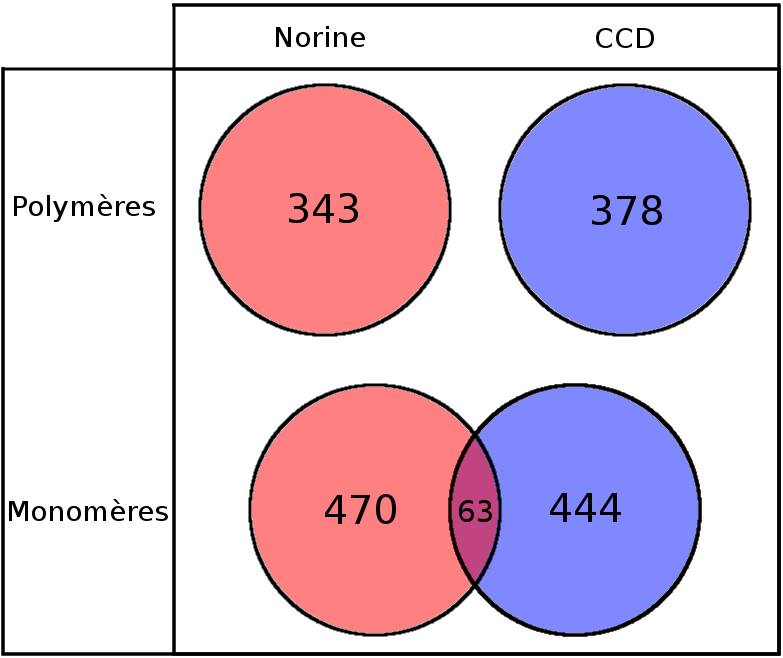
\includegraphics[width=250px]{Figures/s2m/results/data.png}
    \caption{\label{data}Répartition des données de validation}
  \end{center}
\end{figure}



\subsection{Profil d'un résultat}

s2m permet de générer des résultats sous différents formats.
Il est possible par exemple de générer un format textuel \textit{json} permettant facilement de recharger ces résultats dans d'autres logiciels.
Lorsque nous présenterons un résultat, nous le présenterons via le format graphique \textit{html}.

\begin{figure}[!ht]
  \begin{center}
    \includegraphics[width=450px]{Figures/s2m/results/apicidinC.png}
    \caption{\label{s2m_HTML}Le résultat HTML de l'exécution de s2m sur l'apicidine C}
  \end{center}
\end{figure}

Une page de résultat peut être décomposée en 3 parties (voit figure \ref{s2m_HTML}).
En haut à gauche se trouve l'image du polymère étudié, colorée selon les monomères qui y sont présents.
C'est l'information la plus immédiate car elle permet d'immédiatement visualiser un résultat.

Sous l'image du peptide se trouvent trois listes de monomères.
La première liste correspond aux monomères découverts dans la structure atomique par s2m et que l'on sait être justes grâce aux annotations déjà connues.
Le seconde liste correspond également aux monomères découverts par s2m mais qui ne sont pas présents dans l'annotation initiale.
La dernière correspond aux monomères qui sont présents dans l'annotation mais qui n'ont pas été trouvés par s2m.

La partie restante de la figure représente les informations générales sur le polymère.
Tout d'abord, il y a le nom du polymère puis les statistiques sur celui-ci.
La première statistique est le taux de couverture atomique (Coverage).

\begin{equation}
  \text{Coverage} = \frac{\text{nb atomes couverts}}{\text{nb atomes}}
\end{equation}


Cette valeur donne le ratio des atomes annotés par s2m comme faisant partie des monomères trouvés par le nombre d'atomes du polymère.
La seconde valeur appelée \textit{correctness}, donne également un ratio d'atomes mais uniquement pour les atomes correctement annotés.

\begin{equation}
  \text{Correctness} = \frac{\text{nb atomes couverts correctement}}{\text{nb atomes}}
\end{equation}

Cette valeur ne prend en compte que les atomes faisant partie des monomères de la première des trois listes.
Lors de la présentation des résultats, nous ferons toujours attention de bien mentionner si les valeurs sont des comptages monomériques ou des comptages atomiques.
Les écarts entre ces deux valeurs peuvent être très importants à cause de la variabilité du nombre d'atomes composant les monomères.





\subsection{Choix des paramètres}

\label{parameters_choice}

Nous allons tout d'abord nous poser la question du choix des bons paramètres pour effectuer nos tests.
Nous reviendrons d'abord sur la façon de fixer le paramètre d'apprentissage pour le pré-calcul.
Rappelons que, de ce paramètre, découlera le temps de calcul pour les peptides mais que la qualité des résultats ne variera pas.
Puis nous parlerons de la qualité des résultats obtenus en exécutant le programme pour plusieurs paramètres.
Enfin nous étudierons le temps de calcul pour estimer les rapports temps/qualité et ainsi pouvoir recommander les meilleurs calibrations de l'outil.

\subsubsection{Choisir le k du pré-calcul}
\label{k_res}

Pour rappel, l'isomorphisme de sous-graphe est effectué à partir de chaînes pré-calculées afin d'optimiser le temps de recherche (voir partie \ref{index_markov}).
Ces chaînes sont formées de deux sous-parties.
La première sous-partie, de taille k, est optimale en temps de calcul selon une base d'apprentissage.
La seconde sous-partie est générée de manière gloutonne.

Nous allons ici faire varier ce paramètre k et tester les temps de calcul sur les jeux de données.
Pour ne pas parasiter la mesure du temps, nous allons désactiver toutes les autres optimisations logicielles qui augmentent l'efficacité.

\begin{figure}[!ht]
  \begin{center}
    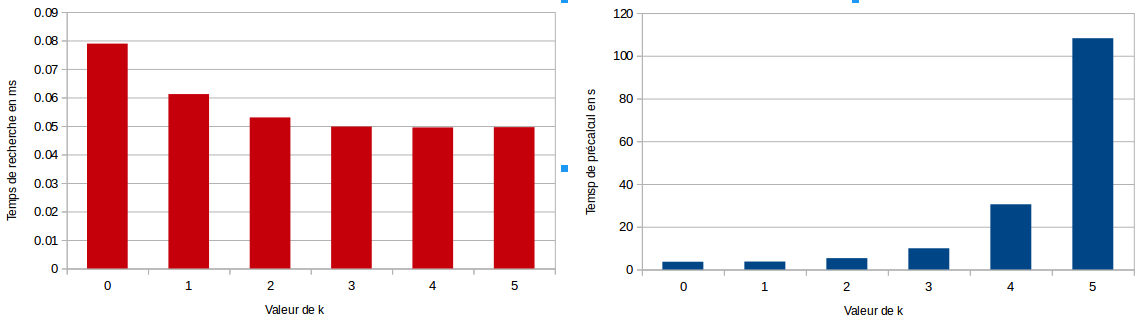
\includegraphics[width=450px]{Figures/s2m/results/k.png}
    \caption{\label{k_graph}Évaluation de l'efficacité d'apprentissage des chaînes sur l'ensemble des monomères des deux jeux de données.
    A gauche : représentation du temps de recherche moyen d'une chaîne dans un peptide selon k.
    A droite : temps d'apprentissage pour tous les monomères selon k.}
  \end{center}
\end{figure}

Observons les résultats sur le schéma \ref{k_graph}.
Le graphique de gauche représente le temps d'exécution moyen d'un isomorphisme (ie recherche d'une chaîne dans un peptide) en fonction de k.
Le graphique de droite représente le temps d'apprentissage en fonction du k.

Quels que soient les valeurs de k, la recherche est très rapide.
On parle ici en centièmes de millisecondes.
Lorsque la chaîne est entièrement générée de manière gloutonne, chaque isomorphisme prend environ 8 centièmes de ms.
Ce temps descend à 5 centièmes à partir d'un k valant 3.
Ce résultat est très intéressant car il nous montre qu'en moyenne seuls les 3 premiers n\oe{}uds sont utiles pour l'optimisation des chaînes sur nos jeux de données.
Les monomères non trouvables dans un peptide donné (même ceux étant constitués de plusieurs dizaines d'atomes), peuvent déjà tous être éliminés après 3 atomes si les chaînes sont correctement formées.
Il n'est donc pas nécessaire de pré-calculer (sur nos données) des chaînes avec un k supérieur à 3.
Ce pré-calcul fait gagner près de 35\% d'efficacité à chaque recherche de SI.


\subsubsection{Mesures}

Classiquement, lorsque l'on souhaite évaluer les résultats d'une prédiction, on utilise les statistiques découlant des vrais/faux positifs/négatifs.
Commençons par définir chacune de ces catégories dans notre cas :
\begin{itemize}
 \item Vrai positif (VP) : Un vrai positif est obtenu lorsque le résultat de la prédiction est identique au résultat attendu.
Dans notre cas, une annotation peptidique est un VP si tous les monomères présents dans l'annotation de s2m sont également présents au sein de l'annotation biologique et inversement.
Nous aurons donc une couverture et un \textit{correctness} de 100\%.
 \item Faux positif (FP) : Un faux positif est obtenu lorsque le résultat de la prédiction parait correct mais qu'il diffère du résultat attendu.
Dans notre cas, une annotation est un FP si tous ses atomes sont couverts par l'annotation mais que celle-ci diffère du jeu test.
Nous aurons donc une couverture de 100\% et un \textit{correctness} inférieur à 100\%
 \item Faux négatif (FN) : Un faux négatif est obtenu lorsque le résultat ne parait pas correct alors qu'il est possible d'en obtenir un correct.
Dans notre cas, une annotation est un FN lorsque nous n'arrivons pas à produire une annotation complète du peptide.
C'est à dire que nous aurons une couverture et une \textit{correctness} inférieure à 100\%.
 \item Vrai négatif (VN) : Un vrai négatif est obtenu lorsque le résultat ne parait pas correct et qu'il n'est pas possible d'en obtenir un.
Dans notre cas, les annotations test sont correctes, ce n'est pas possible.
Il est toujours possible d'obtenir une annotation couvrante vu qu'elles sont toutes présentes dans le jeu test.
\end{itemize}


\subsubsection{Exécutions sur les jeux de données}

\label{resultats_s2m_p}

Pour le choix des paramètres, nous n'allons pour le moment pas prendre en compte le temps d'exécution.
Les but ici est d'exposer uniquement la qualité des résultats.
Pour cela nous allons prendre comme indicateurs la \textbf{couverture atomique moyenne}, le \textbf{correctness atomique moyen} et les taux de VP/FP/FN.
Nous allons faire varier le paramètre du nombre de d'exécution maximal de la branche \textit{light} (R) ainsi que la profondeur de modulation pour le pavage avec modulation (M).
Nous testerons également les deux algorithmes de pavage (MIP et heuristique).

\begin{table}[!ht]
  \centering
  \begin{tabular}{|c|c|c|c|c|c|c|c|c|}
    \hline
    & \multicolumn{4}{c|}{Heuristique} & \multicolumn{4}{c|}{MIP} \\
    \hline
    Params (R-M) & FN & FP & VP & Sensibilité & VP & FP & FN & Sensibilité \\
    \hline
    1 - 1 & 69 & 56 & 217 & 0.759 & 243 & 68 & 31 & 0.887 \\
    \hline
    2 - 1 & 69 & 56 & 217 & 0.759 & 243 & 68 & 31 & 0.887 \\
    \hline
    1 - 2 & 30 & 62 & 250 & 0.893 & 243 & 68 & 31 & 0.887 \\
    \hline
    2 - 2 & 26 & 63 & 253 & 0.907 & 243 & 68 & 31 & 0.887 \\
    \hline
    3 - 3 & 26 & 63 & 253 & 0.907 & 243 & 68 & 31 & 0.887 \\
    \hline
  \end{tabular}
  \caption{\label{nor_results}Résultats de s2m sur les données de Norine.
  Dans la première colonne se trouvent les binômes des valeurs des paramètres retry (R) et modulation (M)}
\end{table}

\begin{figure}[!ht]
  \begin{center}
    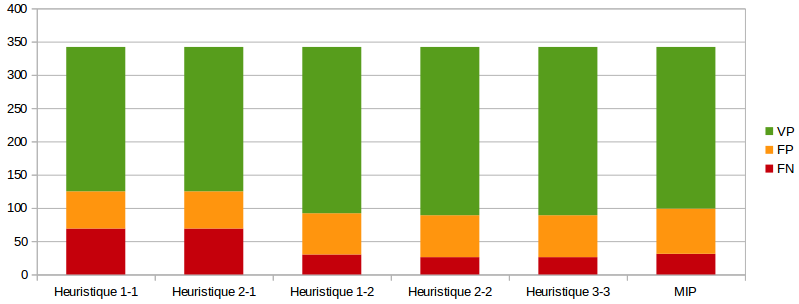
\includegraphics[width=450px]{Figures/s2m/results/Norine.png}
    \caption{\label{nor_graph}Diagramme en barre des résultats sur Norine}
  \end{center}
\end{figure}

\begin{table}[!ht]
  \centering
  \begin{tabular}{|c|c|c|c|c|c|c|c|c|}
    \hline
    & \multicolumn{4}{c|}{Heuristique} & \multicolumn{4}{c|}{MIP} \\
    \hline
    Params (R-M) & FN & FP & VP & Sensibilité & VP & FP & FN & Sensibilité \\
    \hline
    1 - 1 & 45 & 44 & 289 & 0.865 & 310 & 56 & 12 & 0.963 \\
    \hline
    2 - 1 & 45 & 44 & 289 & 0.865 & 310 & 56 & 12 & 0.963 \\
    \hline
    1 - 2 & 10 & 50 & 318 & 0.970 & 310 & 56 & 12 & 0.963 \\
    \hline
    2 - 2 & 9 & 51 & 318 & 0.972 & 310 & 56 & 12 & 0.963 \\
    \hline
    3 - 3 & 9 & 51 & 318 & 0.972 & 310 & 56 & 12 & 0.963 \\
    \hline
  \end{tabular}
  \caption{\label{ccd_results}Résultats de s2m sur les données de CCD.
  Dans la première colonne se trouvent les binômes des valeurs des paramètres retry (R) et modulation (M)}
\end{table}

\begin{figure}[!ht]
  \begin{center}
    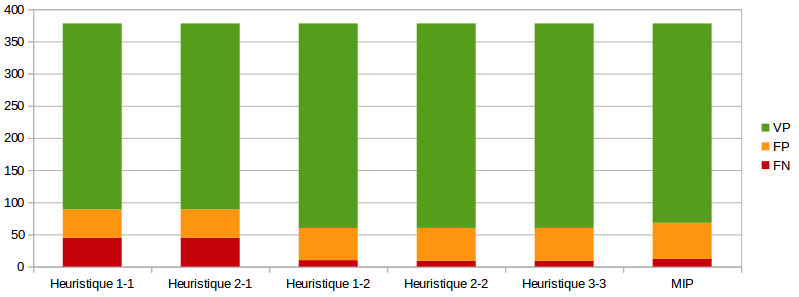
\includegraphics[width=450px]{Figures/s2m/results/CCD.png}
    \caption{\label{ccd_graph}Diagramme en barre des résultats sur CCD}
  \end{center}
\end{figure}


Comme présenté au sein des tableaux \ref{nor_results} et \ref{ccd_results}, l'algorithme de pavage par optimisation linéaire n'est pas du tout sensible aux changements de paramètres.
Ceci s'explique par le fait qu'il n'a besoin que d'une seule phase \textit{light} pour parvenir à son optimal local.
En effet, dans certains cas, le problème est tout de suite résolu après la première phase de pavage succédant à l'isomorphisme \textit{light} car touts les monomères ont été correctement découverts.
Dans les autres cas, l'algorithme du MIP effectue une sur-optimisation après le premier pavage.
Lorsqu'il n'est pas possible d'btenir une couverture complète, l'algorithme a parfois recours à des placement de nombreux petits monomères.
La solution est alors tellement éloignée de l'optimal qu'il devient innateignable pour notre construction algorithmique.

Pour le pavage heuristique, la sensibilité aux paramètres est élevée.
On peut voir que l'augmentation du nombre de modulations déclenche une augmentation du nombre de VP.
Le nombre de vrais positifs augmente significativement en passant le paramètre de 1 à 2.
Cette sensibilité s'explique par le fait que la solution optimale et la solution gloutonne ne sont pas immédiatement voisines.
Il est souvent nécessaire de déplacer, non pas un, mais deux monomères pour atteindre l'optimal.
Le paramètre de nombre de boucle \textit{light} n'a que très peu d'influence et vient seulement compléter 3 résultats sur les données Norine et un seul sur les données de CCD.

En comparant les résultats des deux algorithmes, on s'aperçoit que l'algorithme comprenant l'heuristique de pavage obtient de meilleurs résultats (pour une modulation $\ge$ 2) que l'algorithme incluant un pavage exact.
A nouveau, ce résultat s'explique par le fait que le pavage exact va trop loin dans l'optimisation.
Si aucune solution totalement couvrante n'est possible avec les résidus issus de l'isomorphisme \textit{strict}, alors le pavage maximal exact ira parfois créer des solutions globalement optimisées mais éloignées de la réalité.
Dans ce cas, la recherche de résidus par isomorphisme \textit{light} sert peu car les trous dans l'annotation ont été déplacés par l'optimisation.
Il n'est souvent plus possible de construire l'annotation réelle, à moins de déplacer de nombreux résidus.

Au final, les résultats obtenus sont globalement meilleurs en utilisant l'heuristique gloutonne de pavage avec une modulation de profondeur 2 et deux phases de recherche light.
Nous ne nous attendions pas à ces résultats et la sur-optimisation du pavage par MIP nous a surpris.
Il est tout de même possible d'obtenir des résultats au moins aussi bons qu'avec l'heuristique, en effectuant uniquement une phase de recherche light à la place de la recherche stricte.
Cependant le temps de calcul se voit multipli par 10 sur nos données.


\subsubsection{Temps de calcul global}

\begin{figure}[!ht]
  \begin{center}
    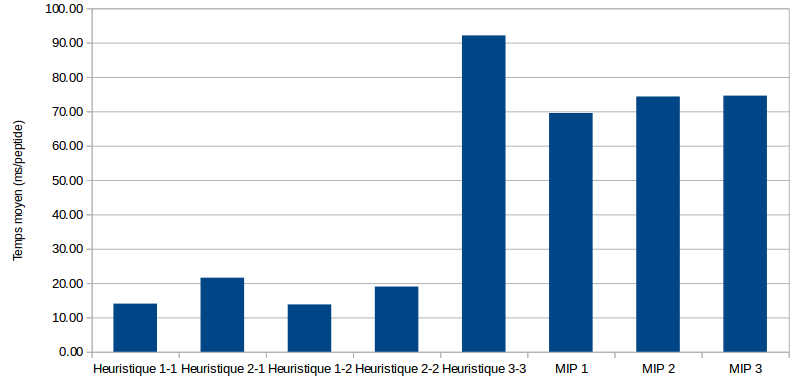
\includegraphics[width=400px]{Figures/s2m/results/temps.png}
    \caption{\label{temps_general}Temps d'exécution moyen par peptide (en ms) en utilisant les deux pavages et différents paramètres pour chacun d'eux.}
  \end{center}
\end{figure}

Pour choisir un bon jeu de paramètres, il ne faut pas prendre que les résultats en considération, mais également le temps qu'il faut pour les générer.
Pour cela, nous avons effectué une analyse comparative des algorithmes en utilisant les différents paramètres cités précédemment.
Comme nous pouvons le remarquer sur le schéma \ref{temps_general}, l'heuristique de pavage obtient un temps d'exécution beaucoup plus faible que le pavage MIP (excepté pour le pavage heuristique 3-3 qui n'a pas d'importance puisqu'il n'apporte pas d'amélioration de qualité).
Ce résultat était attendu mais l'écart expérimental nous pousse fortement à utiliser l'heuristique de pavage plutôt que le MIP sur des données telles que celles présentées ici.

Comparons désormais les temps d'exécution pour l'heuristique en fonction des paramètres passés au programme.
Le paramètre du nombre de boucles \textit{light} semble avoir le plus d'influence sur le temps d'exécution.
C'est à nouveau un résultat que nous attendions puisque la recherche \textit{light} ne s'appuie que sur une faible diversité d'étiquette sur les noeuds (voir les sections \ref{selectiv_p} pour l'influence du nombre d'étiquettes et \ref{light_p} pour la recherche light).
Le temps passé à la recherche de motifs en utilisant les critères \textit{light} est important.
Répéter l'opération plusieurs fois multiplie logiquement le temps d'exécution.

Si l'on regarde bien les temps d'exécution on peut également s'apercevoir que l'augmentation du second paramètre (la profondeur de modulation) permet de diminuer le temps d'exécution.
Ceci peut s'expliquer par les cas où tous les résidus nécessaires à une couverture optimale ont été trouvés mais qu'ils n'ont pas été pavés.
Si la profondeur de modulation nécessaire à l'inclusion de ces résidus n'est pas atteinte, alors le l'algorithme va continuer et perdre du temps, et ce, malgré le fait qu'il aurait pu directement trouver la solution.

Pour conclure cette partie  sur la sélection des paramètres, nous pouvons dire que nous recommandons l'utilisation de l'algorithme de pavage heuristique par rapport au pavage MIP.
Cependant, il ne faut pas utiliser n'importe quels paramètres.
Pousser les paramètres de modulation ou de nombre de boucle à 3 ou au delà est parfaitement inutile en terme de qualité de résultats et consommera énormément de temps.
Utiliser un paramètre de modulation de 1 sera également une erreur puisque la qualité des résultats ne sera pas au rendez-vous.
Il reste finalement deux alternatives intéressantes pour des données du même type que les notre.
Soit nous privilégions la qualité à la vitesse et nous réglons les deux paramètres à la valeur 2, soit nous acceptons de perdre quelques bons résultats au profit de 30\% d'économie de temps en réglant uniquement la modulation à 2.





\subsection{Répartition des temps de calcul et analyse}
\label{temps_calcul}

Maintenant que nous avons choisi les paramètres, analysons attentivement chacune des étapes pour comprendre les points critiques et préparer de futures améliorations.
Pour cela, nous avons exécuté le logiciel sur tous les peptides des jeux test en utilisant un pavage heuristique, une valeur de k à 3, une modulation de 2 et un nombre de tour de boucle de 2.
Pour chacun des peptides, nous avons stocké séparément les temps pour l'isomorphisme strict, le light, le pavage et la modulation.
Les résultats sont affichés sur la figure \ref{temps_calcul}.
Les résultats sont triés par taille de peptide (nombre d'atomes).

\begin{figure}[!ht]
  \begin{center}
    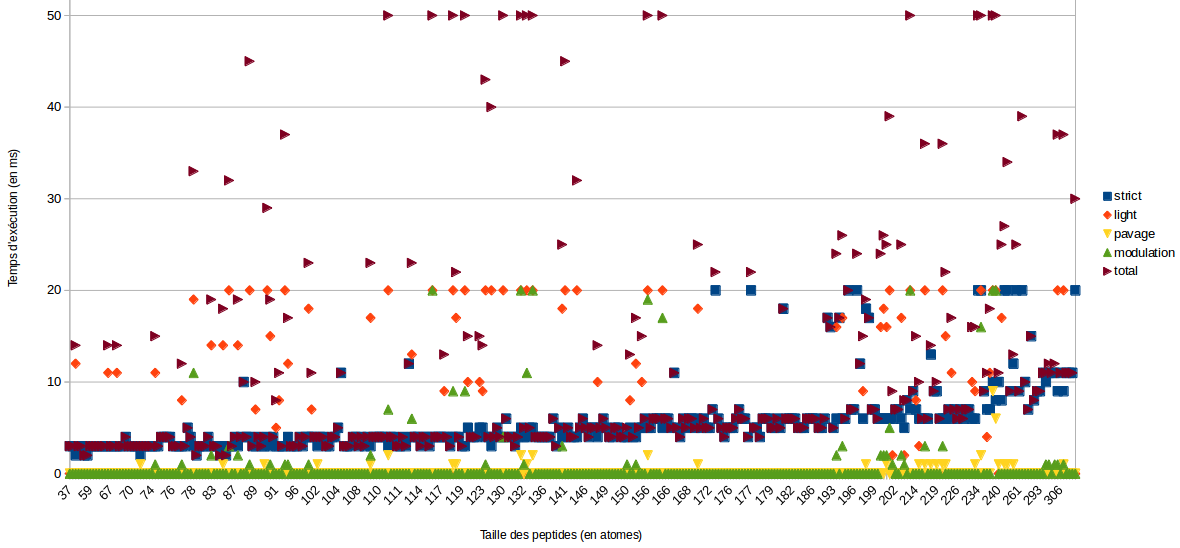
\includegraphics[width=450px]{Figures/s2m/results/temps_detail.png}
    \caption{\label{temps_calcul}Temps d'exécution de s2m pour un extrait aléatoire de 350 molécules.
    Les données ont été tronquées au delà de 50ms pour ne pas écraser le graphique.}
  \end{center}
\end{figure}

Certains points de la figure ont été tronqués car ils écrasaient les résultats.
15 valeurs sur les 350 ont été redescendues à 50ms alors que certaines allaient jusqu'à plusieurs centaines de ms (Le point max atteint 1s à lui seul).
On distingue nettement deux comportements différents sur cette courbe.
Soit les peptides ont été complètement analysés à la suite d'une seule passe de pavage (celle succédant la recherche stricte) ; dans ce cas, le temps d'exécution épouse une courbe qui augmente progressivement avec le nombre d'atomes ; soit le matching \textit{light} et la modulation qui suit entrent en action et le temps devient fortement dépendant de la topologie du peptide (tous les points disparates).

Pour ce qui est de la première catégorie de peptide, on peut voir que la quasi-intégralité du temps est dépensé sur la recherche d'isomorphismes de sous-graphe.
Comme nous le supposions au début de ce projet, les isomorphismes sont des goulots d'étranglement du fait de la complexité des algorithmes de résolution.
Pour quelques peptides, le temps est complété par une phase de modulation qui ne prend que quelques millisecondes.
Dans le pire des cas, le temps est doublé par cette modulation.
L'étape de pavage ne prend jamais plus de 3ms et n'est pas un problème pour le temps d'exécution.

Pour les points de la seconde catégorie, c'est encore l'étape de recherche qui prend le plus de temps.
Cette fois-ci, ce sont les étapes de recherche \textit{light} qui prédominent le temps de calcul.
Comme nous l'avions évoqué lors de la présentation de cette amélioration, le manque d'étiquettes disponibles diminue fortement l'efficacité de l'algorithme.
En moyenne, un isomorphisme \textit{light} est de 10 à 100 fois plus lent qu'un strict.
De plus, les cas qui posent problème sont très souvent accompagnés de longues exécutions de modulation.
Cependant, cet allongement du temps d'exécution permet de résoudre la majorité des cas.
Sur l'extrait des peptides ici présent, seuls 20 d'entre eux finissent sur des impasses.
Toutes les autres exécutions s'arrêtent en obtenant 100\% de couverture.

Pour finir cette analyse des temps de calcul individuels, nous allons parler des cas extrêmes.
Ces cas pathologiques masquent les réelles performances du logiciel.
La moyenne de temps d'exécution globale est de 18ms par peptide mais lorsque nous retirons les 15 cas qui débordent de la figure, cette moyenne chute à 10ms.
À eux seuls, ces 15 peptides représentent plus de la moitié du temps d'exécution du logiciel.
Le cas le plus critique (avoparcin-beta) représente à lui seul un cinquième du temps d'exécution total (plus de 1s).
C'est une structure composée de beaucoup de cycles et d'embranchements. De plus, la structure atomique que nous possédons est fausse, ce qui rend impossible une couverture à 100\%.
L'algorithme passe énormément de temps en boucles \textit{light} et en modulation.
Nous pouvons en conclure qu'il faut éviter d'utiliser des boucles \textit{light} sur des données dont les couvertures ne sont vraiment pas bonnes initialement.
Si nous souhaitons par exemple analyser à l'aveugle un très grand nombre de molécules, il est préférable de se restreindre à une utilisation basique du logiciel, quitte à venir affiner les résultats intéressants par la suite.








\subsection{Analyse des résultats}
\label{res_analyse}

Pour analyser les résultats, nous avons exécuté s2m avec l'algorithme de pavage heuristique.
La profondeur de modulation paramétrée à 2 et le nombre de passage par une phase \textit{light} à 2 également.
Vous trouverez tous les résultats sur les polymères testés à ces adresses :
- CCD : www.TODO.com
- Norine : www.TODO.com


Revenons sur les chiffres qui ont été présentés dans les tableaux \ref{nor_results} et \ref{ccd_results}.
Un peu plus de 74\% des annotations peptidiques issues de Norine et 85\% de celles de CCD sont entièrement retrouvées par le logiciel.
Mais il faut ici rappeler que les annotations ne sont plus considérées comme correctes dès lors qu'au moins un monomère est faussement annoté.
En regardant le taux d'atomes correctement attribués au sein des peptides, le taux de réussite augmente à plus de 93\% pour les annotations de Norine et plus de 98\% pour CCD.

Cependant, même ces très bons taux de réussite ne sont pas représentatifs de la qualité des annotations.
En effet, en analysant les résultats de plus près, nous nous sommes aperçu qu'il était possible de détecter des erreurs au sein des bases de données utilisées pour les tests.
Analysons ensemble plusieurs cas afin de comprendre les raisons de ces erreurs.


\subsubsection{Des peptides aux structures atomiques fausses}

\begin{figure}[!ht]
  \begin{center}
    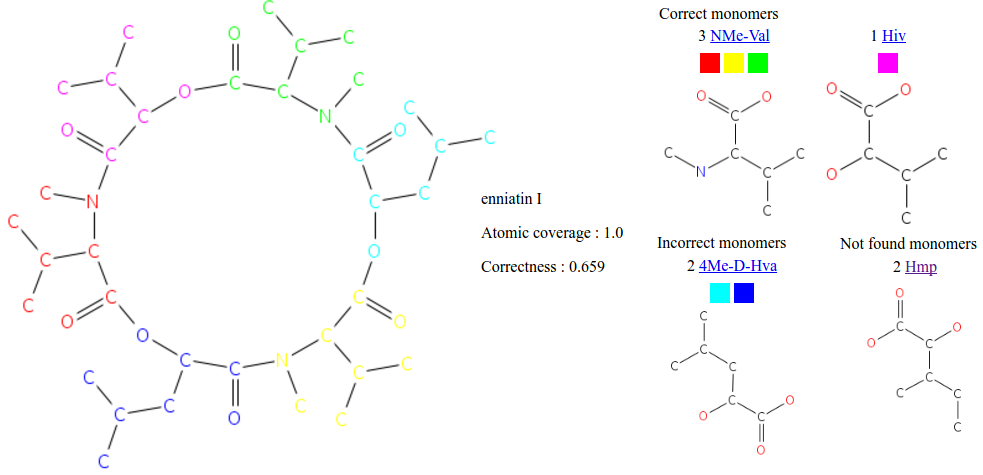
\includegraphics[width=450px]{Figures/s2m/results/s2m_enniati.png}
    \caption{\label{s2m_enniati}Résultat de s2m pour l'enniatin I.
    Deux monomères sont annotés faux ce qui nous mène à dire qu'une erreur s'est glissée soit dans le SMILES de la molécule soit dans l'annotation monomérique.}
  \end{center}
\end{figure}

Beaucoup d'annotations fausses proviennent d'erreurs de structures atomiques pour les peptides.
Prenons l'exemple de l'\textit{enniatin I} (voir figure \ref{s2m_enniati}).
L'annotation en sortie de s2m présente une couverture de 100\% mais un \textit{correctness} de 66\%.
En regardant les 3 listes de monomères, on peut s'apercevoir que l'annotation attendue comporte deux monomères nommés Hmp alors que le logiciel trouve deux 4Me-Hva.
Les deux monomères se ressemblant et il est fort probable que, soit l'annotation monomérique, soit l'annotation atomique ait été mal saisie.
Pour comprendre l'erreur, remontons aux sources des données.
Sur la page Norine de la molécule, nous trouvons un lien vers Pubchem pour nous permettre d'obtenir la structure atomique et un lien vers la publication qui nous permet d'obtenir la structure monomérique.

\begin{figure}[h!]
  \begin{center}
    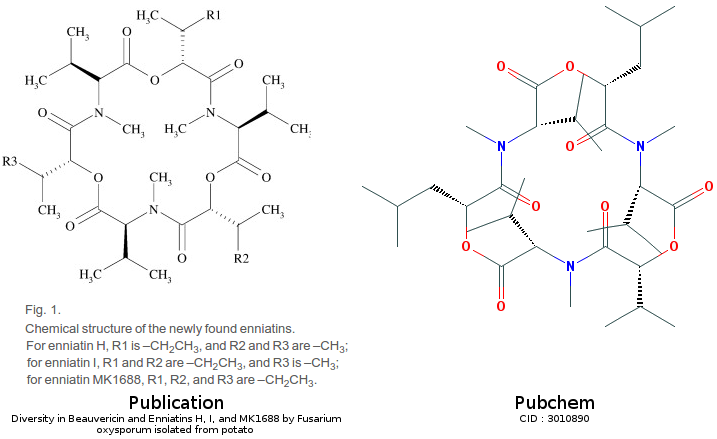
\includegraphics[width=400px]{Figures/s2m/results/enniatinI_corrections.png}
    \caption{\label{enni_cor}Structures atomiques publiées de l'enniatin I.
    Ces deux structures nous aident à déceler une erreur dans la structure atomique de l'enniatin I sur Norine.}
  \end{center}
\end{figure}

En regardant la molécule présente sur PubChem (voir figure \ref{enni_cor}), nous pouvons constater que c'est effectivement la structure atomique qui a été utilisée pour le test.
En consultant le contenu de la publication~\cite{song_diversity_2008}, on s'aperçoit que la structure monomérique correspond à ce qui est présent sur Norine.
Accompagnant cette annotation monomérique est présent un schéma de la structure atomique.
Cette seconde structure vient également confirmer la structure monomérique.
Sans aucun doute, l'erreur provient des données issues de PubChem.
A priori le lien PubChem entré sur Norine n'est pas le bon et pointe vers un peptide similaire.

Nous n'avons pas fini de traiter manuellement toutes les données issues de s2m mais au moins 50\% des erreurs sont de ce type.


\subsubsection{Des monomères aux structures atomiques fausses}

\label{dolastatin_p}

\begin{figure}[h!]
  \begin{center}
    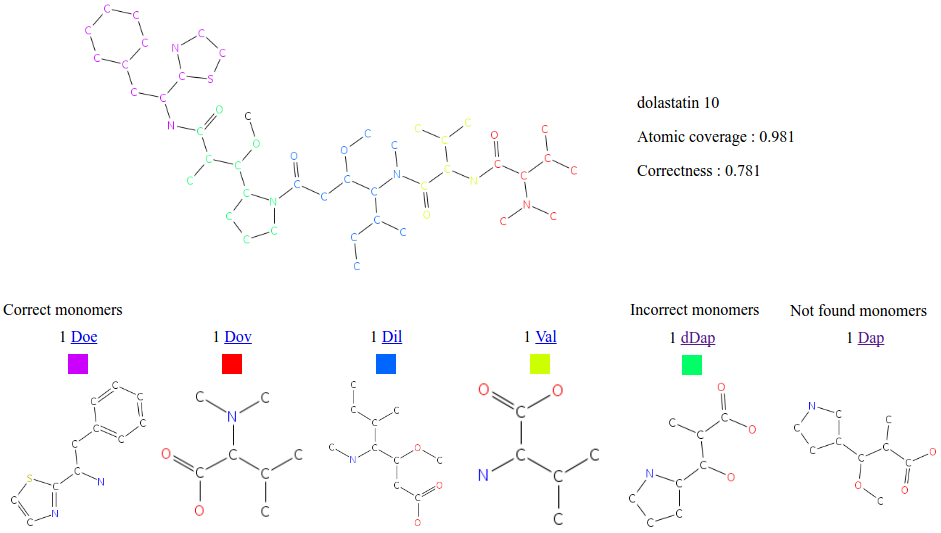
\includegraphics[width=450px]{Figures/s2m/results/dolastatin.png}
    \caption{\label{dolas}Résultat de s2m pour la Dolastatin (peptide de Norine).
    Une erreur de SMILES de monomère empêche une couverture totale du peptide.}
  \end{center}
\end{figure}

Lorsque le taux de couverture de l'annotation issue de s2m est inférieur à 100\%, par définition, au moins un monomère n'a pu être trouvé.
Il est possible que ce monomère n'ait jamais été répertorié, que la structure atomique du peptide soit incorrecte ou que la structure d'un monomère le soit également.
Dans le cas de l'annotation de la dolastatin (voir figure \ref{dolas}), c'est une erreur de structure atomique qui s'est glissée dans la base Norine.
Le monomère Dap qui est sensé être présent n'est pas reconnu car l'atome d'azote n'est pas placé au même endroit au sein du monomère seul et du monomère dans le peptide.
En cherchant sur Norine on peut s'apercevoir qu'aucun autre peptide de la base ne comporte ce monomère, ce qui veut dire qu'il a été ajouté spécifiquement pour ce peptide.
Donc, le changement de structure du monomère n'est a priori pas du à une modification de la molécule, mais ressemblerait plutôt à une erreur d'annotation.
En parcourant l'article qui publia le peptide~\cite{luesch_isolation_2001} et la structure atomique présente sur PubChem, on s'aperçoit que c'est une erreur de structure atomique uniquement présente sur Norine.


\subsubsection{Erreurs d'annotations}

\begin{figure}[h!]
  \begin{center}
    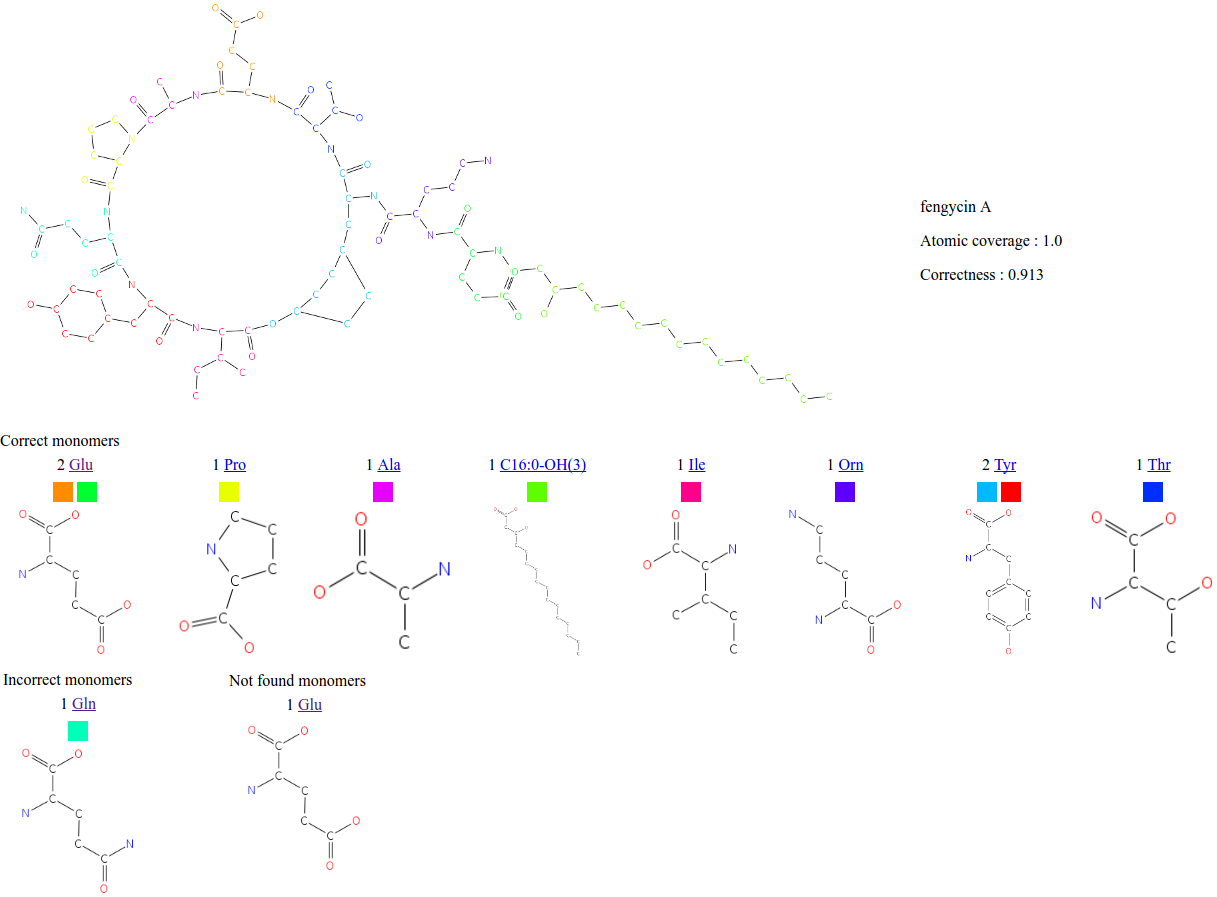
\includegraphics[width=450px]{Figures/s2m/results/fengycin.png}
    \caption{\label{fengycin}Résultat de s2m pour la Fengycin (peptide de Norine).
    Une erreur d'annotation entrée dans Norine réduit la \textit{correctness} alors que s2m trouve la bonne solution.}
  \end{center}
\end{figure}

Il arrive parfois que des molécules soient trompeuses.
En entrant manuellement les annotations, il est possible de confondre un monomère avec un de ses dérivés proches.
C'est ce qui est arrivé avec la fengycine A (voir figure \ref{fengycin}).
L'annotation effectuée par s2m détecte un monomère Gln alors que l'annotation présente dans Norine détecte un Glu.
En effectuant à nouveau toutes les opérations de vérification de la structure atomique et monomérique, on s'aperçoit que l'article~\cite{wu_nonribosomal_2007} donne raison à s2m.
Cette fois-ci, c'est l'annotation monomérique présente dans Norine qui est à changer pour obtenir une information juste.


\subsubsection{Les équivalences}

\begin{figure}[h!]
  \begin{center}
    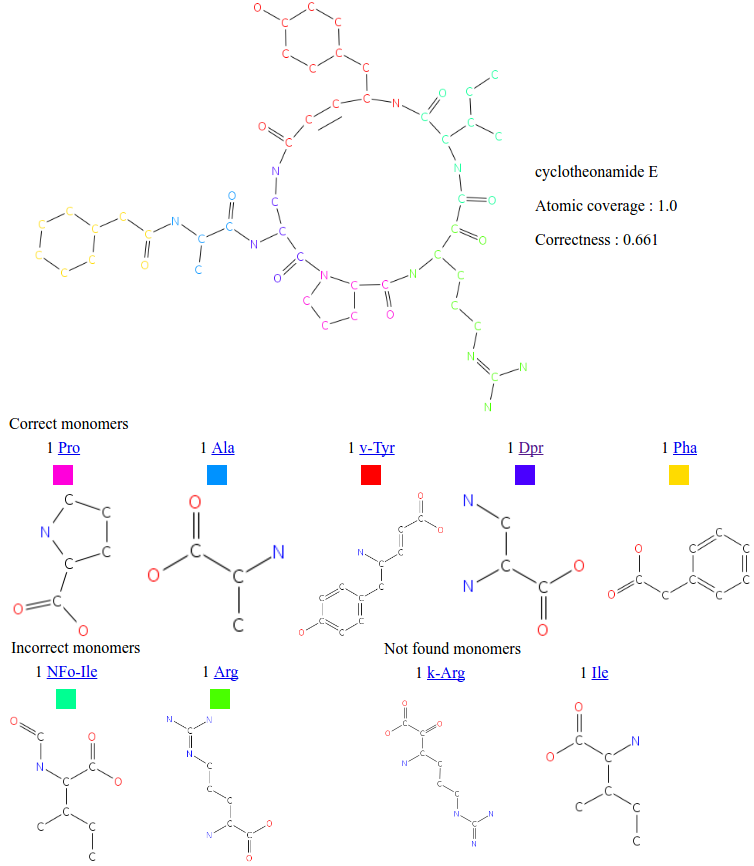
\includegraphics[width=400px]{Figures/s2m/results/cyclotheonamide.png}
    \caption{\label{cycloth}Résultat de s2m pour la Cyclotheonamide E (peptide de Norine).
    L'annotation monomérique recouvre l'entièreté des atomes du peptide mais n'est pas correcte à cause d'une équivalence entre monomères.}
  \end{center}
\end{figure}

Le dernier type d'erreurs d'annotations commises par s2m est strictement du aux algorithmes utilisés pour le pavage.
C'est un problème d'annotations équivalentes.
Comme nous le voyons sur le schéma \ref{cycloth}, la ``cyclotheonamide E'' est un peptide couvert à 100\%.
De plus, l'annotation présente dans Norine propose deux monomères visuellement très proches des monomères suggérés par s2m (Arg/k-Arg et NFo-Ile/Ile).
En regardant dans le détail, on peut observer que c'est un problème du à une formylation entre deux monomères.
L'un des deux monomère a été formylé, ce qui fait qu'un groupement C=O est présent entre les monomères Arg et Ile du peptide.
L'un des monomères a donc été modifié mais il pourrait \textit{a priori} s'agir de celui-ci comme de son variant.
Dans les deux cas, l'annotation qui en résulte reste couvrante à 100\%.
N'ayant aucun moyen algorithmique de faire la différence, ici s2m a choisi la première solution trouvée.
Pour connaître l'annotation réelle, il faut remonter à la production du peptide et comprendre les mécanismes de modification de monomères qui entrent ici en jeu.
Cette erreur est présente moins d'une dizaine de fois dans les données déjà vérifiées et ne pourra pas être corrigée sans prendre en compte plus d'informations biologiques sur le recrutement des monomères.


\subsubsection{Les analyses d'erreur pour CCD}

\begin{figure}[h!]
  \begin{center}
    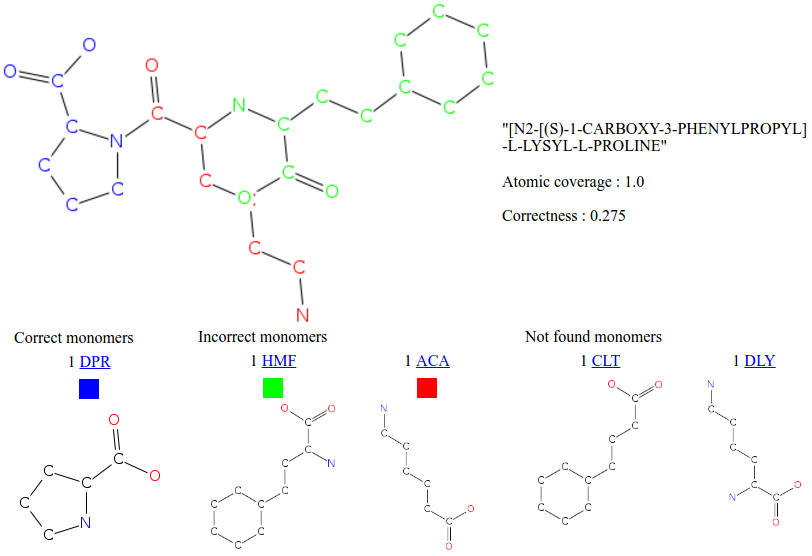
\includegraphics[width=450px]{Figures/s2m/results/CCD_results.png}
    \caption{\label{CCD_results}Équivalence entre monomères.
    L'atome d'azote inclut dans le HME pourrait également être inclus par le DLY mais nous n'avons aucun moyen de faire la différence.}
  \end{center}
\end{figure}

Durant toutes ces analyses, je me suis uniquement attardé sur les erreurs issues des peptides de Norine.
Dans ces cas, il est très facile de vérifier toutes les informations de cette base car de nombreux liens vers les origines des données qui y sont présentes.
Pour les données issues de CCD, nous détectons le même type de problème que dans Norine mais il est très difficile d'analyser chacun d'eux en profondeur.
Nous avons accès aux structures, mais plus difficilement aux publications associées.
Nous pouvons donc également détecter la présence d'erreurs, mais sans forcément pouvoir expliquer leur raison.
Seules les erreurs dues aux équivalences sont facilement détectables (voir par exemple \ref{CCD_results}).
Pour les autres types d'erreurs, nous ne pouvons que spéculer sur leur origine, sans pouvoir vérifier.